%!TEX program = xelatex
\documentclass{xmu}

% ===================== 来自 Report.tex 的附加宏包 =====================
\usepackage{amsthm}
\usepackage{mathrsfs}
\usepackage{float}
\usepackage{multirow}
\usepackage{xcolor}
\usepackage{tcolorbox}
\tcbuselibrary{listings, breakable}
\usepackage{listings}
\usepackage{enumitem}

% ===================== 代码高亮设置 =====================
\lstset{
  language=Python,
  basicstyle=\ttfamily\small,
  keywordstyle=\color{blue!80!black}\bfseries,
  commentstyle=\color{green!50!black}\itshape,
  stringstyle=\color{red!60!black},
  numbers=left,
  numberstyle=\tiny\color{gray},
  numbersep=6pt,
  breaklines=true,
  frame=none,
  showstringspaces=false,
  tabsize=4,
}

% ===================== 定理环境 =====================
\theoremstyle{plain}
\newtheorem{theorem}{定理}[chapter]
\newtheorem{lemma}[theorem]{引理}
\newtheorem{definition}[theorem]{定义}

\theoremstyle{remark}
\newtheorem{remark}[theorem]{注记}
\renewcommand{\proofname}{\bf 证明}

% ===================== 自定义命令 =====================
\newcommand{\norm}[1]{\left\|#1\right\|}
\newcommand{\inner}[2]{\left(#1, #2\right)}
\newcommand{\OmegaBar}{\overline{\Omega}}

\begin{document}

% 基础信息

\print % 电子版 / 打印版（打印版将在某些偶数页产生空白页）
% \arabicchapter % 取消注释后，仅使用数字作为章的编号
% \design % 毕业设计 / 毕业论文（取消注释即为毕业设计）
% \minor % 主修 / 辅修（取消注释即为辅修）
\title{Robust-PINN 求解最优控制问题}{Robust-PINN for Optimal Control Problems}
\author{兰景琪}
\idn{37720222205026}
\college{数学科学学院}
\subject{信息与计算数学}
\grade{2022级}
\teacher{谭志裕\; 助理教授}
\otherteacher{校外指导教师\; 职称} % 注释则不显示校外指导教师
\pubdate{完成时间}
\keywords{物理信息神经网络；最优控制；Scaling；稳定性}{PINN; Optimal Control; Scaling; Stability}

% 封面、承诺书

\maketitle

% 致谢

\begin{acknowledgement}
    致谢内容。
\end{acknowledgement}

% ==================================================================
% 摘要（中文 + 英文）
% 用法：将下方两段内容分别替换主文档中
%   \begin{abstract} ... \end{abstract}
%   \begin{enabstract} ... \end{enabstract}
%   的占位文字。
% ==================================================================

% ===== 中文摘要 =====
\begin{abstract}
偏微分方程约束的最优控制问题在工程优化与反问题中应用广泛。其一阶最优性（KKT）系统中，状态方程与伴随方程通过 $\alpha^{-1}$ 因子耦合（$\alpha$ 为 Tikhonov 正则化参数），当 $\alpha\to 0$ 时该因子使整个鞍点系统呈现严重的尺度失衡。物理信息神经网络（PINN）为该类问题提供了一条无网格、对几何复杂性不敏感的求解路径，然而将其直接施加于 KKT 系统时，未平衡的耦合项使状态网络与伴随网络的参数梯度量级相差 $O(\alpha^{-1})$ 倍，致使优化器在小正则化参数下陷入"平凡核局部极小"——网络同时将状态与伴随压向零的退化解。

本文提出 Robust-PINN 格式从结构层面消除该病态。其核心是将 Brenner--Liu--Sung 在 KKT 鞍点系统多重网格预处理中使用的 $(1/4,-1/4)$ 对角缩放迁移至 PINN 框架：通过变量替换 $\bar y=\alpha^{-1/4}y$、$\bar p=\alpha^{1/4}p$ 与对应的方程行尺度调整，KKT 算子中集中在单一非对角块上的 $\alpha^{-1}$ 因子被对称重分配到全部四个分块。本文从矩阵代数的"对角左右预处理"视角刻画了该缩放的唯一性与结构性，并在加权能量范数 $H_\alpha^1(\Omega)$ 下证明：缩放系统所诱导的双线性形式同时具有连续性与 inf-sup 稳定性，且两个常数均与 $\alpha$ 完全无关。该连续层面的稳定性经链式法则传递至 PINN 雅可比矩阵，使训练梯度在整个 $\alpha$ 范围内保持平衡。

数值实验从原理层（PINN 雅可比的分块 Frobenius 范数、最大奇异值、初始化与训练全程的梯度比率 $\rho$）与现象层（$\alpha$-扫描、$\omega$-扫描下的 $L^2$、$L^\infty$、$H^1$ 相对误差）两个维度系统验证了上述设计：在 $\alpha\in[10^{-5},10^{-2}]$ 全范围内 Robust-PINN 的相对 $L^2$ 误差稳定在 $10^{-3}$ 量级，而未缩放 PINN 在 $\alpha\le 10^{-4}$ 处完全失效；同时还专门解释了未缩放系统失效的具体机制。与 NTK 自适应加权方法的直接对比表明，Robust-PINN 在达到相当或更优精度的同时不引入任何动态超参数与运行时开销，并具备连续层面 inf-sup 稳定性定理的理论保障。
\end{abstract}

% ===== 英文摘要 =====
\begin{enabstract}
Physics-informed neural networks (PINNs) offer a mesh-free, geometry-agnostic alternative to classical finite-element methods for PDE-constrained optimal control. When applied to the first-order optimality (KKT) saddle-point system, however, vanilla PINNs suffer from severe training instability as the Tikhonov regularization parameter $\alpha\to 0$: an $\alpha^{-1}$ coupling term in the system causes the parameter-space gradients of the state and adjoint sub-networks to differ in magnitude by $O(\alpha^{-1})$, driving the optimizer into a \emph{trivial-kernel local minimum} in which both fields collapse toward zero.

This thesis proposes \emph{Robust-PINN} to eliminate this pathology at the structural level. The core idea is to transplant the $(1/4,-1/4)$ diagonal scaling — originally introduced by Brenner, Liu and Sung for multigrid preconditioning of KKT saddle-point systems — into the PINN framework. Under the change of variables $\bar y=\alpha^{-1/4}y$, $\bar p=\alpha^{1/4}p$ together with the corresponding equation-row rescaling, the $\alpha^{-1}$ factor concentrated in a single off-diagonal block of the KKT operator is symmetrically redistributed across all four blocks. We characterize this scaling as a structurally unique two-sided diagonal preconditioner from a matrix-algebraic standpoint, and prove that, in the weighted energy norm $H_\alpha^1(\Omega)$, the bilinear form induced by the scaled system enjoys both continuity and inf-sup stability with constants completely independent of $\alpha$. This continuous-level stability is inherited by the PINN Jacobian via the chain rule, ensuring balanced training gradients across the entire range of $\alpha$.

Numerical experiments validate the method along two complementary axes. At the \emph{principle} level, the Frobenius norms of the Jacobian blocks, the maximum singular value, and the inter-equation gradient ratio $\rho$ remain $\alpha$-independent both at initialization and throughout training. At the \emph{phenomenon} level, $\alpha$- and $\omega$-sweeps show that Robust-PINN maintains relative $L^2$ errors at the $10^{-3}$ level uniformly over $\alpha\in[10^{-5},10^{-2}]$, whereas the unscaled baseline collapses for $\alpha\le 10^{-4}$; a forensic analysis explains the precise mechanism of this failure. A direct comparison against NTK adaptive weighting demonstrates that Robust-PINN achieves comparable or superior accuracy while introducing zero additional hyperparameters, zero runtime overhead, and providing inf-sup stability as theoretical backing.
\end{enabstract}

% 目录

\tableofcontents

% 正文


% ==================================================================
% 第一章：绪论（Introduction）
% 用法：将本文件内容替换主文档中
%       \xmuchapter{绪论}{Introduction}
%       绪论内容（待撰写）。
%   下方的占位段落即可。本章保持与主文档相同的 \xmusection /
%   \xmusubsection / \cite 命令风格，所有引用键均与主文档 bibliography
%   一致（\cite{1} = Tröltzsch；\cite{3} = Gong-Tan-Zhou；
%   \cite{4} = Brenner-Liu-Sung；\cite{21} = Raissi-Perdikaris-Karniadakis；
%   \cite{27} = Wang-Teng-Perdikaris；\cite{29} = Wang-Yu-Perdikaris 等）。

\xmuchapter{绪论}{Introduction}
\label{sec:intro}

\xmusection{研究背景与意义}{Background and Motivation}
\label{subsec:intro-background}

偏微分方程（partial differential equation, PDE）约束的最优控制问题广泛出现在工程与科学的各个领域，例如热传导过程的温度调控、流体的边界驱动、电磁场逆设计、医学影像重建以及参数辨识与逆源问题等等。其一般形式可写为：在某一受 PDE 约束的状态空间中，寻找控制变量 $\bar u$ 使得给定的代价泛函取极小，同时状态变量 $\bar y$ 满足由 $\bar u$ 决定的 PDE 系统~\cite{1}。本文聚焦于其中最经典的一类——线性二次椭圆型分布最优控制问题：
\begin{equation*}
\min_{\bar u}\; J(\bar y, \bar u) = \tfrac{1}{2}\|\bar y - y_d\|^2_{L^2(\Omega)} + \tfrac{\alpha}{2}\|\bar u - u_d\|^2_{L^2(\Omega)},
\quad\text{s.t.}\ -\Delta\bar y = f + \bar u\ \text{in}\ \Omega,\ \bar y|_{\partial\Omega} = 0,
\end{equation*}
其中 $\alpha>0$ 是 Tikhonov 正则化参数。该问题既是最优控制理论的范型问题，又可视为以 $y_d$ 为观测、以 $\bar u$ 为待恢复源项的椭圆逆源问题：当 $\alpha$ 较大时，正则化项主导，问题呈现良好的"控制"特征；而当 $\alpha\to 0$ 时，问题趋向于带数据 $y_d$ 的反问题，正则化项的弱化使整个一阶最优性系统对 $\alpha$ 高度敏感。如何在数值方法层面同时处理"控制"与"反问题"两侧的极限——尤其是在 $\alpha$ 取极小值时仍保持稳定且高精度的求解——是本领域长期以来的核心挑战。

\xmusection{经典数值方法及其参数依赖性}{Classical Numerical Methods and Their Parameter Dependence}
\label{subsec:intro-classical}

经典的求解路径基于一阶最优性条件（KKT 系统）配合有限元方法（finite element method, FEM）。具体来说，引入伴随状态 $\bar p$ 后，原问题等价于求解一组耦合的椭圆鞍点系统（状态方程、伴随方程与最优性条件）。当控制约束不存在时，可通过最优性条件 $\bar u = u_d - \alpha^{-1}\bar p$ 消去控制变量，得到关于 $(\bar y, \bar p)$ 的耦合系统：
\begin{equation*}
-\Delta\bar y + \alpha^{-1}\bar p = f + u_d,\qquad
-\Delta\bar p - \bar y = -y_d.
\end{equation*}
该系统在数值上的核心难点在于：耦合项 $\alpha^{-1}\bar p$ 中的因子 $\alpha^{-1}$ 使得离散后的代数系统条件数随 $\alpha\to 0$ 而爆炸，且状态方程与伴随方程的残差量级在 $\alpha$ 上严重失衡。这种失衡直接影响 FEM 的迭代求解器收敛性、误差估计常数以及自适应算法的最优性。

针对这一问题，Brenner、Liu 与 Sung~\cite{4} 提出了关键的代数性观察：对鞍点系统作变量替换 $\bar y = \alpha^{-1/4}y$、$\bar p = \alpha^{1/4}p$（即缩放指数取 $(1/4,-1/4)$），并对方程作相应行尺度调整，可将 $\alpha^{-1}$ 病态对称地"均分"到耦合系统的四个分块中，得到一个新的等价系统，其分块算子范数全部 $\alpha$-有界。Gong、Tan 与 Zhou 在 \cite{3} 中进一步地系统化了这一思想：他们在该缩放变换的基础上引入加权能量范数
\[
\|v\|_{H_\alpha^1(\Omega)} := \bigl(\|v\|_{L^2(\Omega)}^2 + \alpha^{1/2}\|\nabla v\|_{L^2(\Omega)}^2\bigr)^{1/2},
\]
并在乘积空间 $V = (H_\alpha^1(\Omega))^2$ 上证明了缩放系统所诱导的双线性形式 $\mathcal{K}(\cdot,\cdot)$ 同时具有连续性与 inf-sup 稳定性，且其常数与 $\alpha$ 完全无关。基于这一参数鲁棒的等价 PDE 框架，他们得到了
\begin{itemize}
  \item 关于 $\alpha$ 与 $h$ 一致的 a priori 能量范数与 $L^2$ 范数误差估计；
  \item 上界与下界常数均独立于 $\alpha$ 的 a posteriori 误差估计；
  \item 在初始网格满足 $h_0\alpha^{-1/4}<1$ 假设下自适应有限元算法的收缩性与最优收敛速率。
\end{itemize}
他们的工作首次为这一参数依赖型 KKT 鞍点系统建立了真正与正则化参数无关的数值分析框架。从矩阵代数的角度看，缩放变换正是经典的对角左右预处理（two-sided diagonal preconditioning）\cite{33} 在 KKT 系统上的结构化特殊形式。

\xmusection{物理信息神经网络与最优控制}{Physics-Informed Neural Networks for Optimal Control}
\label{subsec:intro-pinn}

近年来，深度学习方法为 PDE 数值解提供了一条全新的路径。Raissi、Perdikaris 与 Karniadakis 在 \cite{21} 中提出了物理信息神经网络（physics-informed neural networks, PINN）：用一个深度神经网络 $u_\phi(\mathbf{x};\boldsymbol{\theta})$ 直接参数化 PDE 解，并通过最小化 PDE 强残差与边界残差的复合损失
\[
\mathcal{L}(\boldsymbol{\theta}) = \frac{1}{N_r}\sum_{m}|r(\mathbf{x}_m;\boldsymbol{\theta})|^2 + w_{bc}\,\frac{1}{N_b}\sum_{m}|\mathcal{B}u_\phi(\mathbf{x}_m^{\partial\Omega})|^2
\]
来训练网络权重，借助自动微分~\cite{22} 精确计算高阶导数。相较于传统 FEM，PINN 是无网格的、对几何复杂性不敏感、并能自然处理高维与逆问题。其有效性依赖于神经网络的通用逼近能力~\cite{28} 以及自动微分提供的可解析梯度。

将 PINN 推广到最优控制问题有两条自然路径：一是直接以约化代价泛函 $\hat J(\bar u)$ 为目标，通过状态网络的代理求解构造伴随梯度；二是以一阶最优性系统（即 KKT 鞍点系统）的残差为目标，让神经网络同时逼近状态、伴随状态与控制三元组 $(\bar y, \bar p, \bar u)$。后一条路径与 PINN 的标准范式更为一致，也是本文采用的方案。然而，将 PINN 直接应用于 KKT 系统时，正则化参数 $\alpha$ 引入的病态性会以梯度尺度失衡的形式贯穿整个训练过程：未缩放系统中状态网络与伴随网络的参数梯度量级相差 $O(\alpha^{-1})$，使得 Adam~\cite{25}、L-BFGS~\cite{26} 等基于梯度的优化器在 $\alpha$ 较小时无法有效协调两个子网络的更新，最终陷入"平凡核局部极小"——即网络同时将状态与伴随压向零的退化解。

为缓解 PINN 训练中的梯度病态，文献中已发展出若干思路：
\begin{itemize}
  \item \textbf{硬约束架构}：Lagaris 等~\cite{23}、Dong-Ni~\cite{24} 与 Lu 等~\cite{16} 通过距离函数 ansatz $u_\phi = D(\mathbf{x})\mathcal{N}(\mathbf{x};\boldsymbol{\theta})$ 精确施加齐次边界条件，从损失中消除边界惩罚项，从而减少多目标冲突。
  \item \textbf{自适应损失加权}：Wang、Teng 与 Perdikaris~\cite{27,29} 基于神经正切核（NTK）理论提出动态加权策略，在训练过程中根据各残差的 NTK 迹$\mathrm{Tr}(K_k)$ 自动调节权重，依靠 Hutchinson 估计~\cite{30} 实现迹的快速近似。该方法属于"在训练中"动态校正失衡。
  \item \textbf{鲁棒变分框架}：Łoś 与 Paszyński 在最近的工作中指出，标准 PINN 损失 $\sum_x|r(x)|^2$ 与真实 $H_0^1$ 范数误差之间不存在等价关系——损失下降并不保证近似精度提升，使得训练过程缺乏可信的停止准则。他们借鉴有限元方法中的离散弱形式与 inf-sup 稳定性理论，提出 robust loss $\mathrm{LOSS}(\boldsymbol{\theta}) = \mathrm{RES}(\boldsymbol{\theta})^\top G^{-1}\mathrm{RES}(\boldsymbol{\theta})$，其中 $G$ 为关于"使弱形式 inf-sup 稳定"的内积所诱导的 Gram 矩阵。该损失被夹在真实能量范数误差的上下界之间，从而真正成为可信的误差估计器。这一工作清晰地体现了一条原则：\emph{PINN 的损失设计应受底层 PDE 弱形式的 inf-sup 稳定性指导}。
  \item \textbf{配点最小二乘视角}：Weng、Mao 与 Shen 在 \cite{5} 中将 PINN 类方法纳入配点最小二乘（ColloLSQ）框架，并基于残差给出了具有几何收敛率保证的多阶段后验误差控制算法，强调了"先在连续层面消除病态，再实施神经网络近似"的方法论。
\end{itemize}

上述工作虽然角度各异，但有一个共同的方法论核心：\emph{PINN 训练的稳定性，最终由底层连续问题的解析结构（弱形式、范数选取、稳定性条件）所决定}。这一观察为本文的工作奠定了基础。

\xmusection{本文的主要工作}{Main Contributions of This Thesis}
\label{subsec:intro-contrib}

本文将 Brenner--Liu--Sung 的代数缩放与 Gong--Tan--Zhou 的加权 inf-sup 稳定性框架移植到 PINN 求解 KKT 系统的场景中，提出 \emph{Robust-PINN（鲁棒物理信息神经网络）} 格式。本文的主要贡献概括如下。

\textbf{(1) 连续层面的 $\alpha$-平衡 KKT 系统与 inf-sup 稳定性证明.}
本文系统地推导了对原始耦合系统 $(\bar y,\bar p)$ 实施 $(1/4,-1/4)$ 对角缩放后所得的等价 KKT 系统，并从数值线性代数的"对角左右预处理"视角给出该缩放的代数表征：未缩放算子 $\mathcal{A}^{us}$ 集中在单一耦合块上的 $\alpha^{-1}$ 病态，被对称分配到缩放算子 $\mathcal{A}^{sc}$ 的全部四个分块中，使所有分块算子范数 $\alpha$-有界（见第~\ref{sec:part2-scaling}~章定理~\ref{thm:scaling-decomp}）。我们进一步证明了缩放系统所诱导的双线性形式在加权能量范数 $H_\alpha^1(\Omega)$ 下连续且 inf-sup 稳定，常数与 $\alpha$ 无关。

\textbf{(2) Robust-PINN 损失格式.}
基于上述连续层面的稳定性，本文提出针对 KKT 系统的 Robust-PINN 损失：包括缩放后的逐残差归一化、统一的加权能量范数解空间，以及双网络/统一网络两种参数化范式与硬约束/软约束两类边界处理方式所对应的四个损失变体。我们论证了该损失格式在结构上消除了 $\alpha$-病态对参数空间梯度的影响，从而在不引入任何动态超参数与运行时开销的前提下，使 PINN 在小正则化参数下保持稳定训练。

\textbf{(3) 与已有方法的对比定位.}
本文将 Robust-PINN 与未缩放 PINN、NTK 自适应加权 PINN~\cite{27,29} 在统一基准下作系统比较，从原理层（PINN Jacobi分块 Frobenius 范数、最大奇异值、参数空间梯度比率 $\rho$ 在初始化与训练全过程中的演化）与现象层（$\alpha$-扫描、$\omega$-扫描下的相对 $L^2$、$L^\infty$、$H^1$ 误差）两个维度，展示 Robust-PINN 在 $\alpha\in[10^{-5},10^{-2}]$ 全范围内对正则化参数与损失权重均具备数量级的鲁棒性优势，并通过失效模式剖析（见第~\ref{sec:part4-experiments}~章 §\ref{subsec:forensics}）解释了未缩放 PINN 在 $\alpha\le 10^{-4}$ 处的"平凡核局部极小"塌缩现象。

\textbf{(4) 方法论上的统一观点.}
本文的工作进一步印证了一条原则：神经网络求解 PDE 的稳定性问题，其根源往往不在于网络结构或优化器选择，而在于底层连续问题的代数结构。Brenner--Liu--Sung~\cite{4} 与 Gong--Tan--Zhou~\cite{3} 的 inf-sup 稳定性框架原本服务于 FEM 的最优收敛性与 AFEM 最优性证明，而本文展示了同一框架可以无缝地为 PINN 训练提供稳定性背书——这与 Łoś--Paszyński 利用 inf-sup 稳定性构造 robust loss 的思路殊途同归，但路径互补：他们从离散内积的角度构造稳健损失，本文则从连续 PDE 的代数变换角度消除病态。

\xmusection{论文结构}{Organization of the Thesis}
\label{subsec:intro-organization}

本文余下部分组织如下。

第~\ref{sec:part1-continuous}~章给出 PDE 约束最优控制问题的连续形式，推导一阶必要与充分最优性条件，并讨论拉格朗日泛函与 KKT 条件，建立后续章节所需的理论基础。这一部分主要遵循 Tröltzsch~\cite{1} 的经典处理方法。

第~\ref{sec:part2-scaling}~章引入 $(1/4,-1/4)$ 对角缩放，从微分方程层面与矩阵代数层面分别刻画其作用机制（定理~\ref{thm:scaling-decomp}），并在加权能量范数 $H_\alpha^1$ 下证明缩放系统的 inf-sup 稳定性（连续性常数 $C_1=1$、稳定性常数 $c_0=1/\sqrt{2}$，均与 $\alpha$ 无关）。本章为 Robust-PINN 的设计提供了完整的理论支撑。

第~\ref{sec:part3-pinn}~章详细描述 Robust-PINN 的算法：包括状态-伴随对的神经网络参数化（双网络与统一网络）、复合物理信息损失泛函的构建、硬/软约束的边界处理、Adam + L-BFGS 两阶段混合优化策略，以及缩放后的逐残差归一化与去归一化边界损失等实现细节。本章还讨论了梯度比率 $\rho$ 这一原理层诊断量与 NTK 自适应加权~\cite{29} 这一替代路径的关系。

第~\ref{sec:part4-experiments}~章按"原理层—现象层—失效剖析"三层结构开展数值实验：通过 PINN Jacobi分块范数、最大奇异值、参数空间梯度比率以及训练动力学跟踪，验证 Scaling 在结构层面消除 $\alpha$-病态的预测；通过 $\alpha$-扫描与 $\omega$-扫描验证误差指标层面的鲁棒性；通过对失效单元格的网络权重重新加载与可视化，剖析未缩放 PINN 的"平凡核塌缩"机理；最后将本文方法与 NTK 自适应加权~\cite{27} 在相同基准下作直接比较。

\bigskip

\noindent\textbf{记号约定.} 在不引起混淆的前提下，全文使用如下记号：$\Omega\subset\mathbb R^d$（$d\in\{1,2,3\}$）为带 Lipschitz 边界 $\Gamma=\partial\Omega$ 的有界区域；$L^2(\Omega)$ 与 $H_0^1(\Omega)$ 为标准 Sobolev 空间；$(\cdot,\cdot)$ 与 $\|\cdot\|_{L^2(\Omega)}$ 分别表示 $L^2(\Omega)$ 上的内积与范数；$a(v,w):=\int_\Omega\nabla v\cdot\nabla w\,\mathrm dx$；$\bar y, \bar p, \bar u$ 表示原始（未缩放）变量，$y, p, u$ 表示按第~\ref{sec:part2-scaling}~章 §\ref{subsec:balanced-scaling} 中变换 $\bar y = \alpha^{-1/4}y$、$\bar p = \alpha^{1/4}p$ 缩放后的变量。本文中"病态"（ill-conditioning）特指由 $\alpha\to 0$ 引发的算子或梯度尺度失衡，与浮点精度意义下的数值病态相区分。

% ==================================================================
% 第二章：连续问题及其一阶最优性条件（标签已校正）
% ==================================================================
\xmuchapter{连续问题及其一阶最优性条件}{Continuous Problem and First-Order Optimality Conditions}
\label{sec:part1-continuous}

本节给出了偏微分方程约束的最优控制问题的连续形式，并推导对应的一阶必要与充分最优性条件。数学框架遵循Tröltzsch~\cite{1}的经典处理方法，为将在后续章节提出的机器学习方法奠定了理论基础。全文中，$\Omega \subset \mathbb{R}^d$（$d \in \{1,2,3\}$）表示带边界$\Gamma := \partial\Omega$的有界Lipschitz区域，所有函数空间均为标准Sobolev空间意义下的空间。

\begin{remark}
    我们在本节的理论讨论中带边界进行研究，在数值计算阶段，为简化问题，会在全区域上进行数值试验。
\end{remark}

\xmusection{模型问题}{Model Problem}
考虑典型的线性二次椭圆型最优控制问题：寻找最优控制$\bar{u}$，满足
\begin{equation}
\min_{\bar{u} \in U} J(\bar{y}, \bar{u}) := \frac{1}{2} \|\bar{y} - y_d\|^2_{L^2(\Omega)} + \frac{\alpha}{2} \|\bar{u} - u_d\|^2_{L^2(\Omega)},
\end{equation}
约束为椭圆型状态方程
\begin{equation}
\begin{cases}
-\Delta \bar{y} = f + \bar{u} & \text{in } \Omega, \\
\bar{y} = 0 & \text{on } \partial\Omega,
\end{cases}
\end{equation}
其中$U$为控制空间。$y_d \in L^2(\Omega)$为给定的目标状态（即：观测数据），$u_d \in L^2(\Omega)$表示控制$\bar{u}$的先验信息，$f \in L^2(\Omega)$为已知源项，$\alpha > 0$为Tikhonov正则化参数。

代价泛函$J$包含两项：跟踪项$\frac{1}{2}\|\bar{y} - y_d\|^2_{L^2(\Omega)}$，即：惩罚状态与目标观测的偏差；正则化项$\frac{\alpha}{2}\|\bar{u} - u_d\|^2_{L^2(\Omega)}$即：惩罚控制与先验$u_d$的偏差，并保证优化问题的适定性。

称$\bar{y}$为状态变量，$\bar{u}$为控制变量，状态空间为$Y := H^1_0(\Omega)$。

在带控制约束的情形下，将$U$替换为容许集
\begin{equation}
U_{ad} := \bigl\{ u \in L^2(\Omega) : a \le u(x) \le b \text{ 对几乎所有 } x \in \Omega \bigr\},
\end{equation}
其中$a, b \in \mathbb{R}$且$a \le b$。集合$U_{ad}$在$L^2(\Omega)$中非空、闭、有界且凸。

\xmusection{状态方程的适定性与控制-状态算子}{Well-posedness and Control-to-State Operator}
根据Lax–Milgram引理，对任意$u \in L^2(\Omega)$，边值问题(2.2)存在唯一弱解$y = y(u) \in H^1_0(\Omega)$，满足
\begin{equation}
\int_\Omega \nabla y \cdot \nabla v \, dx = \int_\Omega (f + u) v \, dx \quad \forall\, v \in H^1_0(\Omega).
\end{equation}

此外，由Friedrichs不等式，存在仅依赖于$\Omega$的常数$C > 0$，使得
\begin{equation}
\|y(u)\|_{H^1_0(\Omega)} \le C \bigl( \|f\|_{L^2(\Omega)} + \|u\|_{L^2(\Omega)} \bigr).
\end{equation}

\begin{definition}[控制-状态算子]
由(2.2)的唯一弱解定义的映射
$$ G : L^2(\Omega) \to H^1_0(\Omega), \quad u \mapsto y(u), $$
称为控制-状态算子。
\end{definition}

由状态方程的线性性与(2.5)式的先验估计可知，$G$为有界线性算子。由于$H^1_0(\Omega)$在$L^2(\Omega)$为连续嵌入，故而可以引入算子
$$ S := E_Y \circ G : L^2(\Omega) \to L^2(\Omega), $$
其中$E_Y : H^1_0(\Omega) \hookrightarrow L^2(\Omega)$为标准嵌入算子。算子$S$表示直接出现在代价泛函中的控制-状态映射部分。由叠加原理可知，状态可分解为
\begin{equation}
y(u) = S u + y_f,
\end{equation}
其中$y_f := G(f) \in H^1_0(\Omega)$是方程$-\Delta y_f = f$在$\Omega$中、$y_f = 0$在$\partial\Omega$上的解。特别地，$S u = G(u)$对应状态中依赖于控制的部分。

\xmusection{约化问题}{Reduced Problem}
将分解式(2.6)代入代价泛函(2.1)，消去状态变量，得到约化代价泛函
\begin{equation}
\hat{J}(u) := J\bigl(S u + y_f, u\bigr) = \frac{1}{2} \|S u + y_f - y_d\|^2_{L^2(\Omega)} + \frac{\alpha}{2} \|u - u_d\|^2_{L^2(\Omega)}.
\end{equation}

最优控制问题(2.1)–(2.2)等价于约化优化问题
\begin{equation}
\min_{u \in U_{ad}} \hat{J}(u).
\end{equation}

泛函$\hat{J} : L^2(\Omega) \to \mathbb{R}$连续、凸，进一步，由于$\alpha > 0$，事实上泛函$\hat{J}$严格凸。

\begin{theorem}[存在性与唯一性]
设 $U_{ad}$ 在 $L^2(\Omega)$ 中非空、闭、有界且凸，$S : L^2(\Omega) \to L^2(\Omega)$ 是连续线性算子。若 $\alpha > 0$，则约化问题 (2.8) 存在唯一最优解 $\bar{u} \in U_{ad}$。
\end{theorem}

\begin{proof}
由于 $L^2(\Omega)$ 是自反 Hilbert 空间，且 $U_{ad}$ 有界、闭、凸，根据文献 \cite[定理 2.11]{1}，$U_{ad}$ 是弱序列紧的。设 $\{u_n\} \subset U_{ad}$ 是一个极小化序列，满足 $\hat{J}(u_n) \to \inf_{u \in U_{ad}} \hat{J}(u)$。则存在子列 $\{u_{n_k}\}$ 弱收敛于某个 $\bar{u} \in U_{ad}$，即 $u_{n_k} \rightharpoonup \bar{u}$。

由于 $\hat{J}$ 连续且凸，故它是弱下半连续的，因此有：
$$
\hat{J}(\bar{u}) \le \liminf_{k \to \infty} \hat{J}(u_{n_k}) = \inf_{u \in U_{ad}} \hat{J}(u)
$$
又因为 $\bar{u} \in U_{ad}$，故等号成立，从而证明了存在性。唯一性由 $\hat{J}$ 的严格凸性可得，而严格凸性由 $\alpha > 0$ 时的正则化项 $\frac{\alpha}{2}\|u - u_d\|^2$ 保证。
\end{proof}

\begin{remark}
若$U_{ad}$无界（无约束情形$U_{ad} = L^2(\Omega)$），当$\alpha > 0$时存在唯一性仍成立，因为正则化项的强制性可将极小化序列限制在有界集内~\cite{1}。%[定理2.16]
\end{remark}

\xmusection{一阶必要最优性条件}{First-Order Necessary Optimality Condition}
约化泛函(2.7)在$L^2(\Omega)$上Fréchet可微。利用链式法则~\cite{1}与Hilbert空间伴随算子演算，其梯度为
\begin{equation}%2.6
\nabla \hat{J}(u) = S^*(S u + y_f - y_d) + \alpha(u - u_d).
\end{equation}

由于$\hat{J}$凸且Fréchet可微，根据文献~\cite{1}，控制$\bar{u} \in U_{ad}$为最优控制的充要条件是满足变分不等式
\begin{equation}%[引理2.21]
\bigl( \nabla \hat{J}(\bar{u}), u - \bar{u} \bigr)_{L^2(\Omega)} \ge 0 \quad \forall\, u \in U_{ad},
\end{equation}
将(2.9)代入（其中$\bar{y} = S\bar{u} + y_f$），可得
\begin{equation}
\bigl( S^*(\bar{y} - y_d) + \alpha(\bar{u} - u_d), u - \bar{u} \bigr)_{L^2(\Omega)} \ge 0 \quad \forall\, u \in U_{ad}.
\end{equation}

\xmusection{伴随状态}{Adjoint State}
为将抽象变分不等式(2.11)转化为便于计算的PDE系统，引入伴随状态。

\begin{definition}[伴随方程与伴随状态]
给定最优对$(\bar{y}, \bar{u})$，伴随状态$\bar{p} \in H^1_0(\Omega)$是伴随边值问题
\begin{equation}
\begin{cases}
-\Delta \bar{p} = \bar{y} - y_d & \text{in } \Omega, \\
\bar{p} = 0 & \text{on } \partial\Omega.
\end{cases}
\end{equation}
的唯一弱解。
\end{definition}

因$\bar{y} - y_d \in L^2(\Omega)$，由Lax–Milgram引理，伴随方程(2.12)适定。

\begin{lemma}
Hilbert空间伴随算子$S^* : L^2(\Omega) \to L^2(\Omega)$满足：对所有$z \in L^2(\Omega)$，$S^* z = p$，其中$p \in H^1_0(\Omega)$是方程$-\Delta p = z$在$\Omega$中、$p = 0$在$\partial\Omega$上的弱解。
\end{lemma}

\begin{proof}
对任意$z, u \in L^2(\Omega)$，设$y = G(u) \in H^1_0(\Omega)$满足$-\Delta y = u$且$y|_{\partial\Omega} = 0$（仅考虑依赖于$u$的部分），$p \in H^1_0(\Omega)$满足$-\Delta p = z$且$p|_{\partial\Omega} = 0$。分别用$p$测试$y$的方程、用$y$测试$p$的方程，由双线性型对称性得：
$$ \int_\Omega z y \, dx = \int_\Omega \nabla p \cdot \nabla y \, dx = \int_\Omega u p \, dx. $$
即对所有$u \in L^2(\Omega)$，$(z, Su)_{L^2(\Omega)} = (p, u)_{L^2(\Omega)}$，故$S^* z = p$。
\end{proof}

将引理2.6应用于$z = \bar{y} - y_d$，变分不等式(2.11)化为
\begin{equation}
\int_\Omega \bigl( \bar{p}(x) + \alpha\bigl(\bar{u}(x) - u_d(x)\bigr) \bigr) \bigl( u(x) - \bar{u}(x) \bigr) dx \ge 0 \quad \forall\, u \in U_{ad}.
\end{equation}

\xmusection{最优性系统}{Optimality System}
联立状态方程、伴随方程与变分不等式，而控制$\bar{u} \in U_{ad}$及其对应状态$\bar{y}$、伴随状态$\bar{p}$为问题(2.1)–(2.3)最优解的充要条件是三元组$(\bar{y}, \bar{u}, \bar{p})$满足如下最优性系统：
\begin{equation}
\begin{cases}
\textbf{状态方程：} & -\Delta \bar{y} = f + \bar{u} \quad \text{in } \Omega, \quad \bar{y} = 0 \quad \text{on } \partial\Omega, \\[4pt]
\textbf{伴随方程：} & -\Delta \bar{p} = \bar{y} - y_d \quad \text{in } \Omega, \quad \bar{p} = 0 \quad \text{on } \partial\Omega, \\[4pt]
\textbf{最优性条件：} & \bar{u} \in U_{ad}, \quad \bigl( \bar{p} + \alpha(\bar{u} - u_d), v - \bar{u} \bigr)_{L^2(\Omega)} \ge 0 \quad \forall\, v \in U_{ad}.
\end{cases}
\end{equation}

\xmusection{无约束情形与耦合系统}{Unconstrained Case and Coupled System}
当$U_{ad} = L^2(\Omega)$（无控制约束）时，(2.14)中的变分不等式退化为逐点梯度方程
\begin{equation}
\alpha(\bar{u}(x) - u_d(x)) + \bar{p}(x) = 0 \quad \text{对几乎所有 } x \in \Omega,
\end{equation}
由此可得显式表达式
\begin{equation}
\bar{u} = u_d - \frac{1}{\alpha}\bar{p}.
\end{equation}

将(2.16)代入状态方程$-\Delta \bar{y} = f + \bar{u}$，得到关于$(\bar{y}, \bar{p})$的耦合鞍点系统：
\begin{equation}
\begin{cases}
-\Delta \bar{y} = f + u_d - \alpha^{-1}\bar{p} & \text{in } \Omega, \quad \bar{y} = 0 \quad \text{on } \partial\Omega, \\[6pt]
-\Delta \bar{p} = \bar{y} - y_d & \text{in } \Omega, \quad \bar{p} = 0 \quad \text{on } \partial\Omega,
\end{cases}
\end{equation}
由于(2.1)中依赖于先验的正则化项，$u_d$显式出现在第一个方程中。

\begin{remark}[参数依赖性]
系统(2.17)依赖于参数$\alpha$：第一个方程中的$\alpha^{-1}\bar{p}$项与第二个方程中无$\alpha$项，使得两式随$\alpha$变化的尺度行为显著不同。这种失衡对数值方法影响显著，尤其对物理信息神经网络（PINNs），当$\alpha$极小时或极大时，同时约束两个残差会导致训练不稳定。本失衡的矩阵代数刻画与纠正机制，见第~\ref{sec:part2-scaling}~章。
\end{remark}

\xmusection{逐点最优性条件与投影公式}{Pointwise Optimality and Projection Formula}
回到由(2.3)定义$U_{ad}$的带约束问题，(2.14)中的变分不等式等价于如下逐点条件~\cite[引理2.26]{1}：对几乎所有$x \in \Omega$，
\begin{equation}
\bar{u}(x) =
\begin{cases}
a & \text{若 } \bar{p}(x) + \alpha(\bar{u}(x) - u_d(x)) > 0, \\[3pt]
b & \text{若 } \bar{p}(x) + \alpha(\bar{u}(x) - u_d(x)) < 0, \\[3pt]
\in [a, b] & \text{若 } \bar{p}(x) + \alpha(\bar{u}(x) - u_d(x)) = 0.
\end{cases}
\end{equation}

因$\alpha > 0$，可将最优性条件(2.15)解出$\bar{u}$并投影到容许集，得到投影公式
\begin{equation}
\bar{u}(x) = \mathbb{P}_{[a,b]} \left( u_d(x) - \frac{1}{\alpha}\bar{p}(x) \right) \quad \text{对几乎所有 } x \in \Omega,
\end{equation}
其中$\mathbb{P}_{[a,b]}$表示区间$[a,b]$上的逐点投影，
$$ \mathbb{P}_{[a,b]}(z) := \max\bigl\{a, \min\{z, b\}\bigr\}. $$

无约束情形（$a = -\infty$，$b = +\infty$）下，(2.19)退化为(2.16)。

\xmusection{拉格朗日泛函与KKT条件}{Lagrangian and KKT Conditions}
最优性系统(2.14)的等价刻画可由拉格朗日框架给出~\cite{1}。定义拉格朗日泛函$\mathcal{L} : H^1_0(\Omega) \times L^2(\Omega) \times H^1_0(\Omega) \times L^2(\Omega) \times L^2(\Omega) \to \mathbb{R}$为
\begin{equation}
\begin{aligned}
\mathcal{L}(y, u, p, \mu_a, \mu_b) :=&
\frac{1}{2}\|y - y_d\|^2_{L^2(\Omega)} + \frac{\alpha}{2}\|u - u_d\|^2_{L^2(\Omega)} \\
&- \int_\Omega \bigl(\nabla y \cdot \nabla p - (f + u)p \bigr) dx \\
&+ \int_\Omega (a - u)\mu_a dx + \int_\Omega (u - b)\mu_b dx.
\end{aligned}
\end{equation}

一阶最优性（KKT）条件要求存在拉格朗日乘子$\bar{\mu}_a, \bar{\mu}_b \in L^2(\Omega)$在$\Omega$中几乎处处满足$\bar{\mu}_a \ge 0$，$\bar{\mu}_b \ge 0$，使得
\begin{equation}
\begin{aligned}
\nabla_y \mathcal{L} = 0 \quad &\Longleftrightarrow \quad -\Delta \bar{p} = \bar{y} - y_d &&\text{(伴随方程)}, \\[3pt]
\nabla_p \mathcal{L} = 0 \quad &\Longleftrightarrow \quad -\Delta \bar{y} = f + \bar{u} &&\text{(状态方程)}, \\[3pt]
\nabla_u \mathcal{L} = 0 \quad &\Longleftrightarrow \quad \alpha(\bar{u} - u_d) + \bar{p} - \bar{\mu}_a + \bar{\mu}_b = 0 &&\text{(梯度条件)}, \\[3pt]
&\phantom{\Longleftrightarrow}\quad \bar{\mu}_a \ge 0, \quad \bar{\mu}_b \ge 0 &&\text{(对偶可行性)}, \\[3pt]
&\phantom{\Longleftrightarrow}\quad (a - \bar{u}, \bar{\mu}_a)_{L^2} = (\bar{u} - b, \bar{\mu}_b)_{L^2} = 0 &&\text{(互补松弛性)}.
\end{aligned}
\end{equation}

系统(2.21)与原始可行性约束$-\Delta\bar{y} = f + \bar{u}$、$\bar{u} \in U_{ad}$共同构成了最优控制问题(2.1)–(2.3)的Karush–Kuhn–Tucker（KKT）条件。互补松弛性又刻画了积极集$\{x : \bar{u}(x) = a\}$与$\{x : \bar{u}(x) = b\}$的结构，是最优控制正则性理论与数值分析的核心。

\xmusection{与机器学习最优控制框架的联系}{Connection with Machine-Learning Frameworks}
最优性系统(2.14)及其等价形式(2.17)、(2.19)、(2.21)为最优控制问题的机器学习方法提供了解析基础，具体包括：

物理信息神经网络（PINN）方法通过训练神经网络，利用损失函数通过惩罚状态方程、伴随方程与最优性条件的残差，去逼近三元组$(\bar{y}, \bar{u}, \bar{p})$。而将PINN直接应用于耦合系统(2.17)会因方程尺度不匹配而对$\alpha$不稳定。$\alpha$-平衡尺度变换(3.1)导出的系统(3.2)解决了这一问题，得到鲁棒PINN（Robust-PINN）格式。下一节将对这一部分内容做严格说明。

约化形式(2.8)支持构建控制-状态算子$S$的代理模型。训练得到了代理模型$\hat{S} \approx S$后，我们就可以通过梯度法优化近似约化泛函$\hat{J}$，其中梯度(2.9)由伴随方法计算，通过代理模型解析求解或自动微分实现。

而针对于有限的空间来说，投影公式(2.19)为学习解映射中的控制框约束提供了自然实现方式，可作为几乎处处可微层嵌入神经网络，实现约束问题(2.3)的端到端训练。对于更一般的约束，在后续可以有更进一步的研究，例如利用邻近算子格式通过邻近PINN（Prox-PINN）提供类似路径等。

上述联系将在后续章节中详细展开。


% ==================================================================
% 第三章：Scaling 系统及其稳定性分析（标签已校正）
% ==================================================================
\xmuchapter{Scaling 系统及其稳定性分析}{Scaling System and Its Stability Analysis}
\label{sec:part2-scaling}

\xmusection{平衡尺度变换}{Balanced Scaling Transformation}
\label{subsec:balanced-scaling}
为解决注 2.7 指出的参数敏感性问题，引入尺度变换变量\cite{4}
\begin{equation}
y := \alpha^{1/4}\bar{y}, \qquad p := \alpha^{-1/4}\bar{p}.
\end{equation}

将(3.1)代入耦合系统(2.17)（即令$\bar{y} = \alpha^{-1/4}y$，$\bar{p} = \alpha^{1/4}p$），第一式乘以$\alpha^{1/4}$、第二式乘以$\alpha^{-1/4}$，得到平衡最优性系统:
\begin{equation}
\begin{cases}
-\alpha^{1/2}\Delta y + p = \alpha^{3/4}(f + u_d) & \text{in } \Omega, \quad y = 0 \quad \text{on } \partial\Omega, \\[6pt]
-\alpha^{1/2}\Delta p - y = -\alpha^{1/4}y_d & \text{in } \Omega, \quad p = 0 \quad \text{on } \partial\Omega,
\end{cases}
\end{equation}
(3.2)的核心性质是两式关于$\alpha$达到平衡，即微分算子与耦合项在两式中尺度完全一致（分别为$\alpha^{1/2}$与$\alpha^0$），这种处理消除了(2.17)中破坏稳定性的尺度不匹配问题。

另外，平衡系统(3.2)本身是如下尺度变换后最优控制问题的一阶最优性系统
\begin{equation}
\min_{u \in U} \frac{1}{2}\|y - \alpha^{1/4}y_d\|^2_{L^2(\Omega)} + \frac{\alpha}{2}\|u - \alpha^{3/4}u_d\|^2_{L^2(\Omega)}
\end{equation}
约束为
\begin{equation}
\begin{cases}
-\alpha^{1/2}\Delta y = \alpha^{3/4}f + u & \text{in } \Omega, \\
y = 0 & \text{on } \partial\Omega.
\end{cases}
\end{equation}

原始最优控制与状态可由尺度变换量恢复：$\bar{u} = \alpha^{1/4}u$，$\bar{y} = \alpha^{-1/4}y$。


% ------------------------------------------------------------------
% §3.2  Jacobian 矩阵的矩阵分解视角（Task 1，等式编号已校正）
% ------------------------------------------------------------------
\xmusection{Jacobian 矩阵的矩阵分解视角}{Matrix Decomposition Perspective of the Jacobian}
\label{subsec:jacobian-balancing}

上一节从微分方程层面给出了尺度变换 (3.1)；本节从数值线性代数的角度指出：
Scaling 本质上是对系统算子的\emph{左右对角预处理}
（two-sided diagonal preconditioning），其效果是将原系统Jacobian矩阵中集中在
\emph{单个块}上的 $\alpha^{-1}$ 因子，对称地重新分配到所有四个块中，从而消除
块级量纲失衡。这一视角既从数学结构上解释了为何选取指数 $(1/4,-1/4)$
而非其他组合，也直接预测了第~\ref{sec:part4-experiments}~章
§\ref{subsubsec:jacobian} 中 PINN Jocobian矩阵各分块 Frobenius 范数的观测值。

\paragraph{未缩放系统的算子矩阵形式}
将耦合系统 (2.17) 写作关于 $(\bar y,\bar p)^{\top}$ 的线性算子方程
$\mathcal{A}^{us}(\bar y,\bar p)^{\top} = g^{us}$，其中
\begin{equation}
\mathcal{A}^{us} \;:=\; \begin{pmatrix} -\Delta & \alpha^{-1}I \\[2pt] -I & -\Delta \end{pmatrix},
\qquad
g^{us} \;:=\; \begin{pmatrix} f+u_d \\[2pt] -y_d \end{pmatrix}.
\label{eq:A-us}
\end{equation}
$\mathcal{A}^{us}$ 视为作用于 $H_0^1(\Omega)\times H_0^1(\Omega)$ 的分块
算子矩阵；其 $2\times 2$ 块结构中，两个对角块为 Laplace 算子
（算子范数 $O(1)$），非对角块之一为 $-I$（$O(1)$）、另一为 $\alpha^{-1}I$
（$O(\alpha^{-1})$）。这一\emph{单块集中的 $\alpha^{-1}$ 扰动}是 $\alpha\to 0$
时所有下游数值困难（梯度失衡、病态优化、平凡核塌缩）的代数根源。

\paragraph{尺度变换的对角矩阵表达}
定义两个块对角算子矩阵
\begin{equation}
D_L \;:=\; \begin{pmatrix} \alpha^{3/4}I & 0 \\[2pt] 0 & \alpha^{1/4}I \end{pmatrix},
\qquad
D_R \;:=\; \begin{pmatrix} \alpha^{-1/4}I & 0 \\[2pt] 0 & \alpha^{1/4}I \end{pmatrix}.
\label{eq:DLR}
\end{equation}
$D_R$ 实施\emph{变量替换}（列方向缩放）：由 (3.1)，
$\bar y = \alpha^{-1/4}y$、$\bar p = \alpha^{1/4}p$，即
$(\bar y,\bar p)^{\top} = D_R(y,p)^{\top}$。
$D_L$ 实施\emph{方程重标定}（行方向缩放）：状态方程乘以 $\alpha^{3/4}$、
伴随方程乘以 $\alpha^{1/4}$。两者合起来即为由 (2.17) 推导 (3.2) 时所执行
的完整操作。

\begin{theorem}[Scaling 的对角分解]
\label{thm:scaling-decomp}
缩放系统 (3.2) 的算子 $\mathcal{A}^{sc}$ 由未缩放算子 $\mathcal{A}^{us}$
经过左右对角相似变换给出
\begin{equation}
\mathcal{A}^{sc} \;=\; D_L\,\mathcal{A}^{us}\,D_R,
\label{eq:decomp}
\end{equation}
其中 $D_L, D_R$ 由 \eqref{eq:DLR} 定义。进而 $\mathcal{A}^{sc}$ 的四个
分块算子范数满足
\begin{equation}
\|\mathcal{A}^{sc}_{11}\|_{op},\ \|\mathcal{A}^{sc}_{22}\|_{op}
\;=\; O(\alpha^{1/2}),
\qquad
\|\mathcal{A}^{sc}_{12}\|_{op},\ \|\mathcal{A}^{sc}_{21}\|_{op}
\;=\; O(1),
\label{eq:block-bounds}
\end{equation}
即\emph{全部四个块均与 $\alpha^{-1}$ 因子无关}。
\end{theorem}

\begin{proof}
直接矩阵计算：
\begin{align*}
D_L\,\mathcal{A}^{us}\,D_R
&= \begin{pmatrix}\alpha^{3/4}I & 0\\[1pt] 0 & \alpha^{1/4}I\end{pmatrix}
   \begin{pmatrix}-\Delta & \alpha^{-1}I\\[1pt] -I & -\Delta\end{pmatrix}
   \begin{pmatrix}\alpha^{-1/4}I & 0\\[1pt] 0 & \alpha^{1/4}I\end{pmatrix} \\[4pt]
&= \begin{pmatrix}
      -\alpha^{3/4}\Delta & \alpha^{3/4}\!\cdot\!\alpha^{-1}I \\[3pt]
      -\alpha^{1/4}I & -\alpha^{1/4}\Delta
   \end{pmatrix}
   \begin{pmatrix}\alpha^{-1/4}I & 0\\[1pt] 0 & \alpha^{1/4}I\end{pmatrix} \\[4pt]
&= \begin{pmatrix}
      -\alpha^{3/4}\!\cdot\!\alpha^{-1/4}\Delta
      & \alpha^{-1/4}\!\cdot\!\alpha^{1/4}I \\[3pt]
      -\alpha^{1/4}\!\cdot\!\alpha^{-1/4}I
      & -\alpha^{1/4}\!\cdot\!\alpha^{1/4}\Delta
   \end{pmatrix} \\[4pt]
&= \begin{pmatrix}-\alpha^{1/2}\Delta & I\\[3pt] -I & -\alpha^{1/2}\Delta\end{pmatrix}
   \;=\; \mathcal{A}^{sc},
\end{align*}
最后一步与 (3.2) 的算子矩阵形式完全一致。
\eqref{eq:block-bounds} 的分块范数估计由上述显式表达立即可见：非对角块的
系数恰为 $\pm I$（$\alpha$ 指数\emph{完全相互抵消}），对角块的系数为
$\alpha^{1/2}\Delta$（随 $\alpha\to 0$ 单调趋零而保持有界）。
\end{proof}

\paragraph{关键机制：$\alpha^{-1}$ 的对称均分}
\eqref{eq:decomp} 以代数方式揭示了 Scaling 的作用机制：
\emph{将单块集中的 $\alpha^{-1}$ 病态，对称地重分配到四个块}。
逐块追踪 $\alpha$ 指数的汇合过程：

\begin{center}
\begin{tabular}{c|c|c|c}
\toprule
分块位置 & $D_L$ 贡献 & $D_R$ 贡献 & 与 $\mathcal{A}^{us}_{ij}$ 相乘后 \\
\midrule
$(1,1)$: 对角 & $\alpha^{3/4}$ & $\alpha^{-1/4}$ & $\alpha^{1/2}\cdot(-\Delta)$ \\[1pt]
$(1,2)$: 耦合 & $\alpha^{3/4}$ & $\alpha^{1/4}$ & $\alpha\cdot\alpha^{-1}I = I$ \\[1pt]
$(2,1)$: 耦合 & $\alpha^{1/4}$ & $\alpha^{-1/4}$ & $\alpha^{0}\cdot(-I) = -I$ \\[1pt]
$(2,2)$: 对角 & $\alpha^{1/4}$ & $\alpha^{1/4}$ & $\alpha^{1/2}\cdot(-\Delta)$ \\
\bottomrule
\end{tabular}
\end{center}

注意 $(1,2)$ 位置上的 $D_L, D_R$ 贡献合为 $\alpha$，恰好消去
$\mathcal{A}^{us}_{12}$ 中的 $\alpha^{-1}$；$(2,1)$ 位置上两者贡献合为
$\alpha^{0}=1$，保持 $\mathcal{A}^{us}_{21}=-I$ 不变。\emph{只有}指数
$(1/4,-1/4)$ 能使两个非对角块的 $\alpha$ 因子\emph{同时}抵消为 $\alpha^{0}$：
任何其他同类型对角组合都会在某一块上留下非零 $\alpha$ 幂次。这说明
Brenner--Liu--Sung~\cite{4} 选取的 $(1/4,-1/4)$ 并非启发式，而是消除
KKT 鞍点系统 $\alpha^{-1}$ 失衡的\emph{唯一}
对角平衡方案。

\paragraph{PINN Jacobi的继承性}
上述分析在连续层面进行。现在说明它如何直接预测 PINN 网络Jacobi的行为。
在 PINN 框架下，用两个独立网络分别参数化 $\bar y_\phi,\bar p_\phi$，
PDE 残差为 $r = \mathcal{A}\,\mathbf{u}_\phi - g$；
残差对参数的Jacobi由链式法则给出
\begin{equation}
J \;=\; \frac{\partial r}{\partial\phi}
\;=\; \mathcal{A}\cdot \frac{\partial \mathbf{u}_\phi}{\partial\phi},
\label{eq:jacobian-chain}
\end{equation}
其中 $\partial\mathbf{u}_\phi/\partial\phi$ 在标准初始化（如 Xavier、Kaiming）
下是一个与 $\alpha$ \emph{完全无关}的矩阵——其统计行为仅由网络权重的初始
分布决定。因此 $J$ 的分块结构\emph{直接继承}自 $\mathcal{A}$ 的分块结构。
对未缩放系统，$\|J_{12}^{us}\|_F\propto\alpha^{-1}$；对缩放系统，
全部块 Frobenius 范数满足
\[
  \|J_{11}^{sc}\|_F,\ \|J_{22}^{sc}\|_F = O(\alpha^{1/2}),
  \qquad
  \|J_{12}^{sc}\|_F,\ \|J_{21}^{sc}\|_F = O(1),
\]
与 $\alpha^{-1}$ 因子无关。这正是第~\ref{sec:part4-experiments}~章
§\ref{subsubsec:jacobian} 图~\ref{fig:block-norms} 所观察到的现象：
定理~\ref{thm:scaling-decomp} 在\emph{连续}层面给出的块尺度预测，
与在\emph{离散}网络上的 Frobenius 范数测量（六个数量级范围内斜率
精确为 $+1$ 或 $0$）定量吻合。

\begin{remark}[与经典矩阵平衡的联系]
\eqref{eq:decomp} 属于数值线性代数中的\emph{对角平衡}\cite{33}
（matrix balancing / equilibration）的经典处理方式：给定矩阵 $A$，寻找对角矩阵
$D_L, D_R$ 使 $D_L A D_R$ 的行、列范数尽量均衡、条件数尽量小。
本文的特殊性在于：对角矩阵的指数\emph{不是}由数值条件数极小化数值求得，
而是由 KKT 系统的代数结构——即 $\alpha$ 在耦合项 $\alpha^{-1}\bar p$
中的出现方式——\emph{结构性地}决定。这种\emph{结构驱动}的预处理在
连续层面实施，不引入任何运行时开销，不破坏 PDE 的变分形式，
因此完整保持后续 §\ref{subsec:inf-sup-stability} 证明 inf-sup 稳定性
所需的全部空间与算子结构。
\end{remark}


\xmusection{缩放系统的弱形式与联合变分框架}{Weak Form and Unified Variational Framework of the Scaled System}
\label{subsec:weak-form}

对于缩放后的一阶最优性系统：
\begin{equation*}
  \begin{cases}
  -\alpha^{1/2}\Delta y + p = \alpha^{3/4}(f+u_d) & \text{in } \Omega \\
  -\alpha^{1/2}\Delta p - y = -\alpha^{1/4}y_d & \text{in } \Omega
  \end{cases}
\end{equation*}
并伴随齐次 Dirichlet 边界条件 $y=0, p=0$ on $\partial\Omega$。

利用测试函数 $w \in H_0^1(\Omega)$，$v \in H_0^1(\Omega)$ 构建等价的弱形式系统：
\begin{equation}
  \begin{cases}
  \alpha^{1/2}(\nabla p, \nabla w) - (y, w) &= -\alpha^{1/4}(y_d, w) \quad \forall w \in H_0^1(\Omega) \\
  (p, v) + \alpha^{1/2}(\nabla y, \nabla v) &= \alpha^{3/4}(f+u_d, v) \quad \forall v \in H_0^1(\Omega)
  \end{cases}
\end{equation}

最优控制问题的一阶必要条件是由关于 $y$的状态方程和关于 $p$的伴随状态方程组成的一个相互耦合的系统。为了对其进行整体的泛函分析，引入联合解空间 $V := (H_\alpha^1(\Omega))^2$ 和联合测试函数 $(w, v)$，将这两个方程的弱形式叠加，构造出了一个紧凑的$H_{0}^{1}(\Omega)\times H_{0}^{1}(\Omega)$ 上的全局双线性形式 $\mathcal{K}((y, p), (w, v))$，其中
\begin{equation}
  \begin{cases}
  \mathcal{K}((y,p),(w,v))&:=\alpha^{1/2}a(w,p)-(y,w)+(p,v)+\alpha^{1/2}a(y,v)\\
  g(w,v)&:=-\alpha^{1/4}(y_{d},w)+\alpha^{3/4}(f+u_{d},v)
  \end{cases}
\end{equation}
（注：$a(v,w):=\int_{\Omega}\nabla v\cdot\nabla w~dx$ $\forall v,w\in H_{0}^{1}(\Omega)$）

这种构造的依据是将复杂的耦合 PDE 问题转化为一个标准的单一变分问题：
\begin{equation}
  \mathcal{K}((y, p), (w, v)) = g(w, v)
\end{equation}
其中，通过这种紧凑的表达方式，可以更直接地应用inf-sup 理论来证明这一鞍点问题的稳定性以及统一变量$y$与$p$的解空间。

\xmusection{加权能量范数}{Weighted Energy Norm}
\label{subsec:weighted-norm}

为了衡量误差和系统的稳定性，我们定义依赖于参数 $\alpha$ 的加权能量范数 $H_\alpha^1(\Omega)$：
\begin{equation}
  \|v\|_{H_\alpha^1(\Omega)} := \left( \|v\|_{L^2(\Omega)}^2 + \alpha^{1/2}\|\nabla v\|_{L^2(\Omega)}^2 \right)^{1/2}
\end{equation}
并且将在乘积空间 $V$ 上的组合范数定义为：
\begin{equation}
  \|(y,p)\|_V := \left( \|y\|_{H_\alpha^1(\Omega)}^2 + \|p\|_{H_\alpha^1(\Omega)}^2 \right)^{1/2}
\end{equation}

\xmusection{Inf-sup 稳定性}{Inf-sup Stability}
\label{subsec:inf-sup-stability}

\begin{lemma}
  对于由式 (3.11) 导出的双线性形式 $\mathcal{K}(\cdot, \cdot)$，存在独立于 $\alpha$ 的正常数 $c_0$ 和 $C_1$，使得：
  \begin{equation}
  c_0 \|(y,p)\|_V \le \sup_{(w,v)\in V} \frac{\mathcal{K}((y,p),(w,v))}{\|(w,v)\|_V} \le C_1 \|(y,p)\|_V
  \end{equation}
\end{lemma}

\begin{proof}
  \textbf{(1) 证明双线性形式的连续性（上限 $C_1$）：}

  利用柯西-施瓦茨不等式（Cauchy-Schwarz inequality），我们对双线性形式的绝对值进行放缩：
  \begin{align*}
  \mathcal{K}((y,p), (w,v))
  &=\alpha^{1/2}a(w,p)-(y,w)+(p,v)+\alpha^{1/2}a(y,v)\\
  &\le \|y\|_{L^2} \|w\|_{L^2} + \alpha^{1/2}\|\nabla p\|_{L^2} \|\nabla w\|_{L^2} + \|p\|_{L^2} \|v\|_{L^2} + \alpha^{1/2}\|\nabla y\|_{L^2} \|\nabla v\|_{L^2}
  \end{align*}

  应用离散的柯西-施瓦茨不等式 $\sum a_i b_i \le \sqrt{\sum a_i^2}\sqrt{\sum b_i^2}$，可得：
  \begin{align*}
  \mathcal{K}((y,p), (w,v)) &\le \left(\|y\|_{L^2}^2 + \alpha^{1/2}\|\nabla y\|_{L^2}^2 + \|p\|_{L^2}^2 + \alpha^{1/2}\|\nabla p\|_{L^2}^2 \right)^{1/2} \\
  &\quad \cdot \left(\|w\|_{L^2}^2 + \alpha^{1/2}\|\nabla w\|_{L^2}^2 + \|v\|_{L^2}^2 + \alpha^{1/2}\|\nabla v\|_{L^2}^2 \right)^{1/2}
  \end{align*}

  化简后即为：
  \begin{equation}
  \mathcal{K}((y,p), (w,v)) \le \|(y,p)\|_V \cdot \|(w,v)\|_V
  \end{equation}

  这证明了连续性，且上限常数 $C_1 = 1$。

  \medskip
  \textbf{(2) 证明 inf-sup 下界稳定性条件（下限 $c_0$）：}

  为证明$c_0 \|(y,p)\|_V \le \sup_{(w,v)\in V} \frac{\mathcal{K}((y,p),(w,v))}{\|(w,v)\|_V}$，即证明存在测试函数$w_0$,$v_0$使得存在$c_0 \|(y,p)\|_V \le \frac{\mathcal{K}((y,p),(w_0,v_0))}{\|(w_0,v_0)\|_V}$。\\

  则对于任意给定的 $(y,p) \in V$，构造特定的测试函数：令 $w = p - y$ 以及 $v = p + y$。\\

  代入双线性形式展开：
  \begin{align*}
  \mathcal{K}((y,p), (p-y, p+y)) &= \alpha^{1/2}(\nabla p, \nabla(p-y)) - (y, p-y) + (p, p+y) + \alpha^{1/2}(\nabla y, \nabla(p+y)) \\
  &= \alpha^{1/2}(\nabla p, \nabla p) - \alpha^{1/2}(\nabla p, \nabla y) - (y,p) + (y,y) + (p,p) + (p,y) \\
  &\quad + \alpha^{1/2}(\nabla y, \nabla p) + \alpha^{1/2}(\nabla y, \nabla y)\\
  &=(y,y)+ \alpha^{1/2}(\nabla y, \nabla y) + (p,p)+ \alpha^{1/2}(\nabla p, \nabla p)\\
  &=\|y\|_{L^2}^2 + \alpha^{1/2}\|\nabla y\|_{L^2}^2 + \|p\|_{L^2}^2 + \alpha^{1/2}\|\nabla p\|_{L^2}^2 \\
  &= \|(y,p)\|_V^2
  \end{align*}

  计算构造的测试函数范数，由平行四边形法则知:
  \begin{align}
  \|(w,v)\|_V^2
  &= \frac{1}{2}\|p-y\|_{H_\alpha^1}^2 + \frac{1}{2}\|p+y\|_{H_\alpha^1}^2 \\
  &= \frac{1}{2}\|p\|_{H_\alpha^1}^2 +\frac{1}{2} \|y\|_{H_\alpha^1}^2
  \end{align}

  由此可得：
  \begin{equation}
  \frac{\mathcal{K}((y,p), (w,v))}{\|(w,v)\|_V} = \frac{\|(y,p)\|_V^2}{\sqrt{2}\|(y,p)\|_V} = \frac{1}{\sqrt{2}}\|(y,p)\|_V
  \end{equation}

  因此：
  \begin{equation}
  \sup_{(w,v)\in V} \frac{\mathcal{K}((y,p), (w,v))}{\|(w,v)\|_V} \ge \frac{1}{\sqrt{2}} \|(y,p)\|_V
  \end{equation}

  即下界常数 $c_0 = 1/\sqrt{2}$，证明完毕。\cite{3} \cite{6}
\end{proof}

\xmusection{稳定性结论对 PINN 的指导意义}{Implications for PINN}
\label{subsec:pinn-implications}

该引理的证明对于使用物理信息神经网络（PINNs）求解最优控制问题具有决定性的理论指导和算法稳定意义：

\begin{itemize}
  \item 从数学底层消除神经网络训练的"梯度病态"\\
  PINN 的训练过程高度依赖于基于梯度的优化器（本实验中为Adam 及 L-BFGS）来更新网络权重。如果底层的 PDE 系统本身条件数很差（随 $\alpha$→0 爆炸），损失函数的优化地貌将变得极度扭曲，容易导致梯度崩溃或陷入不良的局部最优。而本引理严格证明了该缩放系统在加权范数下，其双线性形式的连续性上界 $C_1$和 inf-sup 稳定性下界$c_0$是完全独立于$\alpha$的。这相当于在连续层面上对物理方程进行了理想的"预处理"，从根本上解耦了系统条件数与$\alpha$的联系，保证了神经网络在计算损失函数梯度时不会因为极小的$\alpha$而引发数值不稳定。

  \item 为设计"Robust-PINN"提供严密的理论背书\\
  正是因为直接用 PINN 求解原始问题存在不稳定性，我们需要一套在理论上无懈可击的新系统来设计算法。本引理证明了缩放后的系统在解空间及其对偶空间之间诱导了一个独立于参数$\alpha$的同构关系。这一泛函分析层面的强有力结论保证了：无论正则化参数多么微小，该系统都不会发生算子退化。这直接促成了鲁棒物理信息神经网络（Robust-PINN）的提出，使得深度学习求解器能够真正胜任惩罚参数极小的复杂最优控制问题。

  \item 统一变量解空间，简化网络架构与权重设计\\
  在应用 PINN 求解最优控制问题时，神经网络通常需要同时输出状态变量 $y$ 和伴随状态变量 $p$。未缩放时，它们的自然范数是不同的（分别带有 $\alpha^{1/2}$ 和 $\alpha^{-1/2}$ 权重）。而本引理证明了经过缩放后，不仅 $y$ 和 $p$ 可以存在于同一个解空间 $V = (H_\alpha^1(\Omega))^2$ 中，而且它们可以完美地共享同一个加权能量范数 $\|(y,p)\|_V$。故而对于 PINN 的实施而言，这意味着神经网络的多个输出在物理量纲和误差尺度上已经达到了天然对齐，从而避免了在损失函数中人工盲目调节不同物理量残差权重的繁琐工作
\end{itemize}


% ==================================================================
% 第四章：物理信息神经网络求解最优控制问题（更新版）
%
% 更新要点（相对于原 Report.tex）：
%   1. 新增 \label{sec:part3-pinn} 供 §5 反向引用
%   2. §3.2.3 比较评估：修正对 "第4节" 的错误引用 → 第5章 §5.3.3
%   3. 变体 I–IV：添加一行"范围说明"，指出哪些是 §5 主体实验、哪些为辅助
%   4. §3.3.6 汇总表：增加"主体使用"列
%   5. §3.4 尺度敏感性：引用第3章新增的定理~\ref{thm:scaling-decomp}
%      以及第5章 §5.2 的雅可比诊断作为验证
%   6. §3.4 权重敏感性：由过去时改为预见性，并引入 ρ 梯度比率诊断
%   7. 新增短段介绍 NTK 自适应加权作为替代路径（\cite{29}），衔接 §5.5
% ==================================================================

\xmuchapter{物理信息神经网络求解最优控制问题}{Physics-Informed Neural Networks for Optimal Control}
\label{sec:part3-pinn}

本章开发基于物理信息神经网络（PINN）的计算框架，用于求解
第 \ref{sec:part1-continuous} 章推导的最优性系统 (1.14)。
该方法包含五个紧密集成的组件：
(i) 状态-伴随对 $(\bar y, \bar p)$ 的神经网络参数化；
(ii) 复合物理信息损失泛函的构建；
(iii) 通过硬约束（假设函数）和软约束（惩罚）架构施加边界条件；
(iv) 结合一阶（Adam）和拟牛顿（L-BFGS）方法的混合优化策略；
(v) 消除第 \ref{sec:part2-scaling} 章中识别的参数依赖性病态的
$\alpha$-平衡尺度变换（定理~\ref{thm:scaling-decomp}）。
所有算法选择均基于第 \ref{sec:part1-continuous}--\ref{sec:part2-scaling}
章的理论框架，其有效性将在第 \ref{sec:part4-experiments} 章通过
系统的数值实验（原理层诊断与现象层鲁棒性）验证。


\xmusection{神经网络架构与变量参数化}{Network Architecture and Variable Parameterization}
\label{subsec:pinn-arch}

使用前馈神经网络对状态 $\bar y$ 和伴随状态 $\bar p$ 进行参数化。
研究两种架构范式：\emph{双网络}架构（$\bar y$ 和 $\bar p$ 由独立网络表示）
和\emph{统一网络}架构（共享隐藏层和二维输出）。

\paragraph{双网络架构（Dual Network）}
设 $\mathcal{N}_y(\mathbf{x};\boldsymbol{\theta}_y):\Omega\to\mathbb{R}$ 和
$\mathcal{N}_p(\mathbf{x};\boldsymbol{\theta}_p):\Omega\to\mathbb{R}$ 分别表示
两个独立的单输出前馈网络，参数向量为 $\boldsymbol{\theta}_y$ 和
$\boldsymbol{\theta}_p$。每个网络的形式为
\begin{equation}
\mathcal{N}(\mathbf{x};\boldsymbol{\theta})
= W^{[L]}\sigma\bigl(W^{[L-1]}\sigma(\cdots\sigma(W^{[1]}\mathbf{x}+\mathbf{b}^{[1]})\cdots)+\mathbf{b}^{[L-1]}\bigr)+\mathbf{b}^{[L]},
\end{equation}
其中 $L$ 表示层数，$W^{[\ell]}\in\mathbb{R}^{n_\ell\times n_{\ell-1}}$ 和
$\mathbf{b}^{[\ell]}\in\mathbb{R}^{n_\ell}$ 是权重矩阵和偏置向量，
$\sigma$ 是逐分量应用的非线性激活函数。在实现中，使用 SiLU 激活\cite{31}
$\sigma(z)=z/(1+e^{-z})$，它提供 $C^\infty$ 光滑性——这是通过自动微分
（AD）计算二阶导数的要求——同时避免了经典 Sigmoid \cite{31}的梯度消失问题
\cite{21}。架构包含 $L=4$ 层（3 个宽度为 50 的隐藏层和 1 个输出神经元），
每个网络的总参数数为 $|\boldsymbol{\theta}_y|=|\boldsymbol{\theta}_p|
=2\cdot 50+50\cdot 50+50\cdot 50+50\cdot 1+(50+50+50+1)=5{,}251$。

\paragraph{统一网络架构（Unified Network）}
或者，定义单个网络 $\mathcal{N}_{yp}(\mathbf{x};\boldsymbol{\theta}):\Omega\to\mathbb{R}^2$，
具有共享隐藏层和二维输出层：
\begin{equation}
\mathcal{N}_{yp}(\mathbf{x};\boldsymbol{\theta})
= \bigl(\mathcal{N}_{yp}^{(1)}(\mathbf{x};\boldsymbol{\theta}),\,
         \mathcal{N}_{yp}^{(2)}(\mathbf{x};\boldsymbol{\theta})\bigr)^\top.
\end{equation}
隐藏层架构与双网络相同（3 个宽度为 50 的隐藏层，SiLU 激活），但最后一层
映射到 $\mathbb{R}^2$。共享表示施加了归纳偏置：状态和伴随在功能上是耦合的
——这与最优性系统 (1.17) 的鞍点性质一致的结构先验。
该架构将总参数数减少到 $5{,}302$（单个共享主体加双输出头）。

\begin{remark}[两种架构在本文中的角色]
\label{rem:arch-scope}
\emph{双网络架构}是第 \ref{sec:part4-experiments} 章数值实验的\emph{主体设置}。
选择它的理由是：参数空间 $\boldsymbol{\theta}_y\cap\boldsymbol{\theta}_p
=\varnothing$ 使得状态-伴随的梯度信号在结构上天然分离，从而能够\emph{干净地}
观测到 $\alpha$-病态通过 KKT 系统的 $\alpha^{-1}$ 耦合项在参数梯度上造成的
失衡（图~\ref{fig:block-norms}、\ref{fig:rho-init}）。
统一网络的参数共享会引入隐式耦合，干扰这一结构信号。
\emph{统一网络}在本章作为理论参照与后续扩展的起点保留，其定性结论与双网络
一致——详见第 \ref{sec:part4-experiments} 章 §\ref{subsec:synthesis} 的简要
验证。
\end{remark}

\paragraph{前向传播与自动微分}
PINN 方法需要在内部配点处评估微分算子 $-\Delta\bar y$ 和 $-\Delta\bar p$。
这些通过反向模式自动微分（AD）精确计算（到机器精度）\cite{22}。
对于 $\mathbf{x}=(x_1,x_2)\in\Omega\subset\mathbb{R}^2$，
网络输出 $u=\mathcal{N}(\mathbf{x};\boldsymbol{\theta})$ 的拉普拉斯算子通过下式获得
\begin{equation}
\Delta u = \sum_{i=1}^{d}\frac{\partial^2 u}{\partial x_i^2},
\qquad
\frac{\partial^2 u}{\partial x_i^2} = \frac{\partial}{\partial x_i}
\!\left(\frac{\partial u}{\partial x_i}\right),
\end{equation}
其中每个偏导数通过调用 AD 引擎并设置 \texttt{create\_graph=True} 来保留
计算图以进行二阶微分。


\xmusection{边界条件处理}{Boundary Condition Handling}
\label{subsec:bc-handling}

齐次 Dirichlet 条件 $\bar y|_{\partial\Omega}=0$ 和 $\bar p|_{\partial\Omega}=0$
的施加可以通过修改网络架构精确实现，也可以通过在损失中添加惩罚项近似实现。
这一选择在定义损失函数之前做出，因为它决定了进入 PDE 残差计算的网络输出
$\bar y_\theta,\bar p_\theta$ 的形式。

\xmusubsection{硬约束：通过假设函数精确施加}{Hard Constraints via Ansatz}
\label{subsubsec:hard-bc}
遵循 Lagaris 等人\cite{23}的距离函数方法及其现代改进\cite{24,16}，
我们将原始网络输出乘以一个在 $\partial\Omega$ 上恒为零的函数。
对于单位正方形 $\Omega=(0,1)^2$，定义
\begin{equation}
D(\mathbf{x}) = x_1(1-x_1)x_2(1-x_2),
\end{equation}
并将试函数设置为
\begin{equation}
\bar y_\theta(\mathbf{x}) = D(\mathbf{x})\mathcal{N}_y(\mathbf{x};\boldsymbol{\theta}_y),
\qquad
\bar p_\theta(\mathbf{x}) = D(\mathbf{x})\mathcal{N}_p(\mathbf{x};\boldsymbol{\theta}_p),
\end{equation}
（或者在统一情况下与 $\mathcal{N}_{yp}$ 的两个输出等价）。通过构造，
对于所有参数值，$\bar y_\theta|_{\partial\Omega}\equiv 0$ 和
$\bar p_\theta|_{\partial\Omega}\equiv 0$。这对后续损失公式有三个重要后果：

\begin{enumerate}[label=\arabic*.]
\item 不需要边界损失。优化简化为仅最小化内部 PDE 残差，
      消除了多目标竞争的一个来源。
\item 竞争损失项的数量减少。硬边界条件变体最多涉及两个损失项
      （每个 PDE 一个），而软边界条件变体涉及三个或更多。
\item 假设函数通过乘积法则在拉普拉斯算子中引入额外项：
      \begin{equation}
      \Delta(D\cdot\mathcal{N}) = D\Delta\mathcal{N}+2\nabla D\cdot\nabla\mathcal{N}+\mathcal{N}\Delta D.
      \end{equation}
      这些额外贡献由 AD 引擎透明处理，不需要手动实现。
\end{enumerate}

\begin{remark}[推广到非矩形域]
假设函数方法通过将 $D(\mathbf{x})$ 替换为任何满足 $D|_{\partial\Omega}=0$
且在 $\Omega$ 中 $D>0$ 的函数，推广到任意域；例如，有符号距离函数
$D(\mathbf{x})=\mathrm{dist}(\mathbf{x},\partial\Omega)$ 或从预训练辅助网络
获得的水平集函数\cite{24}。
\end{remark}

\xmusubsection{软约束：惩罚施加}{Soft Constraints via Penalty}
\label{subsubsec:soft-bc}
当显式假设函数不可用或规定了非齐次边界数据时，通过在损失泛函中添加惩罚项
来施加边界条件。设 $\{\mathbf{x}_m^{\partial\Omega}\}_{m=1}^{M_{\partial\Omega}}\subset\partial\Omega$
为边界配点，均匀采样，每条边 $M_{\partial\Omega}/4$ 个点。直接使用原始
网络输出 $\mathcal{N}_y(\mathbf{x};\boldsymbol{\theta}_y)$ 和
$\mathcal{N}_p(\mathbf{x};\boldsymbol{\theta}_p)$——没有 $D(\mathbf{x})$ 因子
——并且边界不匹配在损失中被惩罚。

在缩放系统中出现一个微妙之处。特征缩放（见 §\ref{subsec:train-strategy}）
分别将原始输出乘以 $\alpha^{1/4}$ 和 $\alpha^{3/4}$。
在精确解消失的边界点处，缩放预测 $\bar y_\theta=\alpha^{1/4}\hat y$ 和
$\bar p_\theta=\alpha^{3/4}\hat p$ 携带这些因子。
如果边界损失直接定义为 $|\bar y_\theta|^2+|\bar p_\theta|^2$，则伴随边界项
尺度为 $O(\alpha^{3/2})$，对于小 $\alpha$ 变得可忽略，从而有效地解耦
$\bar p$ 的边界约束。为了防止这种情况，定义去归一化边界损失
\begin{equation}
\mathcal{L}_{\mathrm{BC}}^{\mathrm{sc}}
= \frac{1}{M_{\partial\Omega}}\sum_{m=1}^{M_{\partial\Omega}}\left[
\left|\frac{\bar y_\theta(\mathbf{x}_m^{\partial\Omega})}{\alpha^{1/4}}\right|^2
+ \left|\frac{\bar p_\theta(\mathbf{x}_m^{\partial\Omega})}{\alpha^{3/4}}\right|^2\right],
\label{eq:bc-loss-sc}
\end{equation}
这将两个项恢复到在 $\alpha$ 上均匀的 $O(1)$。对于未缩放系统，不需要
去归一化：
\begin{equation}
\mathcal{L}_{\mathrm{BC}}^{\mathrm{us}}
= \frac{1}{M_{\partial\Omega}}\sum_{m=1}^{M_{\partial\Omega}}
\bigl[|\bar y_\theta(\mathbf{x}_m^{\partial\Omega})|^2+|\bar p_\theta(\mathbf{x}_m^{\partial\Omega})|^2\bigr].
\label{eq:bc-loss-us}
\end{equation}

\xmusubsection{比较评估}{Comparative Evaluation}
\label{subsubsec:bc-comparison}
第 \ref{sec:part4-experiments} 章的数值实验表明，硬约束架构在所有测试的
$\alpha$ 值上始终优于软约束方法，相对 $L^2$ 误差提高了约一到两个数量级
（Hard BC 下 $L^2\sim 10^{-4}$；Soft BC + 合适的 $w_{bc}\ge 10$ 下
$L^2\sim 10^{-2}$，见 §\ref{subsubsec:softbc} 与图~\ref{fig:wbc-sweep}）。
这一优势可归因于两个因素：
(i) 边界损失的消除消除了优化器中多目标冲突的一个来源；
(ii) 假设函数将结构知识（$\bar y$ 和 $\bar p$ 在 $\partial\Omega$ 上消失）
直接嵌入到假设类中，将网络的表示能力集中在内部解结构上。
这些发现与\cite{24}针对单方程边值问题的观察一致；
但第 \ref{sec:part4-experiments} 章 §\ref{subsubsec:softbc} 的讨论
进一步区分了 Hard/Soft BC 下 Scaling 效果的\emph{适用范围}：
Scaling 处理的是系统\emph{内部}（$\mathrm{eq}_1$ 与 $\mathrm{eq}_2$ 之间）
的失衡，与 PDE-BC 的\emph{跨类}失衡正交，后者由 $w_{bc}$ 独立控制。


\xmusection{损失函数构建}{Loss Function Construction}
\label{subsec:loss-construction}

有了网络架构（§\ref{subsec:pinn-arch}）和边界处理（§\ref{subsec:bc-handling}），
现在构建物理信息损失泛函。损失将最优性系统(2.14)编码为在 $M_\Omega$ 个
内部配点 $\{\mathbf{x}_m^\Omega\}_{m=1}^{M_\Omega}\subset\Omega$ 处施加的
软约束。由于损失结构取决于架构选择和边界处理，因此产生了四种不同的变体；
其中变体 I、III（双网络）将在第 \ref{sec:part4-experiments} 章作为主体
验证对象。

\xmusubsection{PDE 残差（所有变体通用）}{PDE Residual (Common to All Variants)}
\label{subsubsec:pde-residual}

给定根据 §\ref{subsec:pinn-arch} 和 §\ref{subsec:bc-handling} 构造的网络
预测 $\bar y_\theta(\mathbf{x})$ 和 $\bar p_\theta(\mathbf{x})$，最优性系统
的内部 PDE 残差如下。

未缩放系统（参见(2.17)）：
\begin{equation}
r_1^{\mathrm{us}}(\mathbf{x})
:= -\Delta\bar y_\theta-(f+u_d)+\alpha^{-1}\bar p_\theta,
\qquad
r_2^{\mathrm{us}}(\mathbf{x})
:= -\Delta\bar p_\theta-\bar y_\theta+y_d.
\label{eq:res-us}
\end{equation}

缩放系统（参见(2.19)）：
\begin{equation}
r_1^{\mathrm{sc}}(\mathbf{x})
:= -\alpha^{1/2}\Delta y_\theta+p_\theta-\alpha^{3/4}(f+u_d),
\qquad
r_2^{\mathrm{sc}}(\mathbf{x})
:= -\alpha^{1/2}\Delta p_\theta-y_\theta+\alpha^{1/4}y_d.
\label{eq:res-sc}
\end{equation}

即使在缩放系统中，两个残差也具有不同的量级：当 $\alpha\to 0$ 时，
$r_1^{\mathrm{sc}}\sim O(\alpha^{3/4})$ 而 $r_2^{\mathrm{sc}}\sim O(\alpha^{1/4})$。
为了实现完全平衡的残差，应用逐残差归一化
\begin{equation}
\tilde r_1^{\mathrm{sc}} := \frac{r_1^{\mathrm{sc}}}{\alpha^{3/4}},
\qquad
\tilde r_2^{\mathrm{sc}} := \frac{r_2^{\mathrm{sc}}}{\alpha^{1/4}},
\label{eq:res-normalize}
\end{equation}
使得 $\tilde r_1^{\mathrm{sc}},\tilde r_2^{\mathrm{sc}}\sim O(1)$ 在 $\alpha$
上均匀。对于未缩放系统，写 $\tilde r_i=r_i^{\mathrm{us}}$（不应用归一化）。
为了符号简洁，定义逐点均方残差
\begin{equation}
\mathcal{L}_1 := \frac{1}{M_\Omega}\sum_{m=1}^{M_\Omega}|\tilde r_1(\mathbf{x}_m^\Omega)|^2,
\qquad
\mathcal{L}_2 := \frac{1}{M_\Omega}\sum_{m=1}^{M_\Omega}|\tilde r_2(\mathbf{x}_m^\Omega)|^2.
\end{equation}

现在介绍四种损失变体。

\xmusubsection{变体 I——双网络 + 硬边界}{Variant I — Dual Network, Hard BC}
\label{subsubsec:variant-I}
\emph{主体变体}。假设函数(4.6)消除了边界损失，并且不相交的参数
$\boldsymbol{\theta}_y,\boldsymbol{\theta}_p$ 允许对两个 PDE 残差进行独立加权。
损失为
\begin{equation}
\boxed{\;\mathcal{L}^{\mathrm{I}}(\boldsymbol{\theta}_y,\boldsymbol{\theta}_p)
= \gamma\mathcal{L}_1(\boldsymbol{\theta}_y,\boldsymbol{\theta}_p)
+ \mathcal{L}_2(\boldsymbol{\theta}_y,\boldsymbol{\theta}_p),\;}
\label{eq:loss-I}
\end{equation}
其中 $\gamma>0$ 是控制对状态方程与伴随方程相对重视的可调权重。基线配置
使用 $\gamma=1$；在第 \ref{sec:part4-experiments} 章 §\ref{subsubsec:omega-sweep}
的权重敏感性实验中，我们扫描 $\gamma\in\{10^{-2},10^{-1},1,10,10^{2}\}$。

由于 $\boldsymbol{\theta}_y$ 和 $\boldsymbol{\theta}_p$ 不相交，梯度分解为
\begin{equation}
\nabla_{\boldsymbol{\theta}_p}\mathcal{L}^{\mathrm{I}}
= \gamma\nabla_{\boldsymbol{\theta}_p}\mathcal{L}_1
+ \nabla_{\boldsymbol{\theta}_p}\mathcal{L}_2.
\end{equation}
在未缩放系统中，$\nabla_{\boldsymbol{\theta}_p}\mathcal{L}_1$ 包含来自
$r_1^{\mathrm{us}}$ 中耦合项 $\alpha^{-1}\bar p_\theta$ 的因子 $\alpha^{-1}$，
因此 $\gamma$ 直接调节梯度失衡的严重程度——这正是第 \ref{sec:part4-experiments}
章 §\ref{subsubsec:omega-sweep} 测试的核心。

\xmusubsection{变体 II——统一网络 + 硬边界}{Variant II — Unified Network, Hard BC}
\label{subsubsec:variant-II}
\emph{辅助变体}（仅作理论对照）。共享参数向量 $\boldsymbol{\theta}$ 和
假设函数(4.6)产生一种损失，其中两个残差在简化之前聚合成单个向量：
\begin{equation}
\boxed{\;\mathcal{L}^{\mathrm{II}}(\boldsymbol{\theta})
= \frac{1}{2M_\Omega}\sum_{m=1}^{M_\Omega}\bigl(|\tilde r_{1,m}|^2+|\tilde r_{2,m}|^2\bigr)
= \tfrac{1}{2}(\mathcal{L}_1+\mathcal{L}_2).\;}
\label{eq:loss-II}
\end{equation}
这等价于形成连接残差向量
$\mathbf{r}=[\tilde r_{1,1},\ldots,\tilde r_{1,M_\Omega},\tilde r_{2,1},\ldots,\tilde r_{2,M_\Omega}]^\top\in\mathbb{R}^{2M_\Omega}$
并计算 $\mathcal{L}^{\mathrm{II}}=(2M_\Omega)^{-1}|\mathbf{r}|_2^2$。

与\eqref{eq:loss-I}的关键区别是没有每方程权重。每个参数 $\theta_k$ 接收混合梯度
\begin{equation}
\frac{\partial\mathcal{L}^{\mathrm{II}}}{\partial\theta_k}
= \frac{1}{2M_\Omega}\sum_{m}
\biggl(\tilde r_{1,m}\frac{\partial\tilde r_{1,m}}{\partial\theta_k}
+\tilde r_{2,m}\frac{\partial\tilde r_{2,m}}{\partial\theta_k}\biggr),
\end{equation}
并且每个残差的相对贡献由残差量级和共享隐藏层的Jacobi结构共同决定。
这使得逐残差归一化\eqref{eq:res-normalize}在统一架构中更加重要：
没有它，量级较大的残差通过共享参数主导梯度信号。
由于参数共享会将 $\alpha$-病态与架构耦合效应混杂在一起，
\emph{第 \ref{sec:part4-experiments} 章不将此变体作为主体实验}；
其定性表现与变体 I 一致的验证见 §\ref{subsec:synthesis}。

\xmusubsection{变体 III——双网络 + 软边界}{Variant III — Dual Network, Soft BC}
\label{subsubsec:variant-III}
\emph{主体变体}。移除假设函数引入了边界惩罚。对于双网络，三个独立的损失
分量相加：
\begin{equation}
\boxed{\;\mathcal{L}^{\mathrm{III}}(\boldsymbol{\theta}_y,\boldsymbol{\theta}_p)
= \mathcal{L}_1+\mathcal{L}_2+w_{bc}\mathcal{L}_{\mathrm{BC}},\;}
\label{eq:loss-III}
\end{equation}
其中 $\mathcal{L}_{\mathrm{BC}}$ 对未缩放系统由\eqref{eq:bc-loss-us}给出，
对缩放系统由\eqref{eq:bc-loss-sc}给出，$w_{bc}>0$ 为边界惩罚权重。
第 \ref{sec:part4-experiments} 章 §\ref{subsubsec:softbc} 在
$w_{bc}\in\{1,10,100,1000\}$ 与 $\alpha\in\{10^{-2},\ldots,10^{-5}\}$ 上
做二维扫描，以明确界定 Scaling 有效的参数范围。

针对于此变体与硬边界条件的区别，在实现上有一个重要的细节设置：在 Adam 优化阶段，
内部点 $\{\mathbf{x}_m^\Omega\}$ 和边界点 $\{\mathbf{x}_m^{\partial\Omega}\}$
在每个 epoch 动态重采样，提供随机正则化效果，减轻对固定配点配置的过拟合。这种重采样设置使得当边界惩罚在 $\partial\Omega$ 附近产生尖锐损失梯度时特别有益。

\xmusubsection{变体 IV——统一网络 + 软边界}{Variant IV — Unified Network, Soft BC}
\label{subsubsec:variant-IV}
\emph{辅助变体}。在带软边界施加的统一架构中，PDE 残差如
§\ref{subsubsec:variant-II} 那样连接，并且单独的边界组用自己的权重附加：
\begin{equation}
\boxed{\;\mathcal{L}^{\mathrm{IV}}(\boldsymbol{\theta})
= \omega\mathcal{L}_{\mathrm{PDE}}(\boldsymbol{\theta})
+ w_{bc}\mathcal{L}_{\mathrm{BC}}(\boldsymbol{\theta}),\;}
\label{eq:loss-IV}
\end{equation}
其中 $\mathcal{L}_{\mathrm{PDE}}=\tfrac{1}{2}(\mathcal{L}_1+\mathcal{L}_2)$，
$\mathcal{L}_{\mathrm{BC}}$ 为\eqref{eq:bc-loss-us}或\eqref{eq:bc-loss-sc}。
\eqref{eq:loss-IV}的两组结构清晰地将物理（PDE 最优性条件）与约束
（边界数据）分开，直接类似于 DCM 框架的两块配点矩阵\cite[§2.1]{5}：
\begin{equation}
\mathbf{A}
=\begin{pmatrix}\mathcal{L}\phi_n(\mathbf{x}_m)\\[2pt]\lambda\phi_n(\mathbf{x}_m')\end{pmatrix},\quad
\mathbf{b}
=\begin{pmatrix}f(\mathbf{x}_m)\\[2pt]\lambda g(\mathbf{x}_m')\end{pmatrix},
\end{equation}
其中 DCM 惩罚参数 $\lambda$ 在我们的符号中扮演 $\sqrt{w_{bc}/\omega}$ 的角色。
与变体 I、III 不同，\eqref{eq:loss-IV}中的权重 $\omega$ 以相同方式缩放两个
PDE 残差，因为它们共享单个连接向量。由于参数共享与 $\alpha$-病态的
混杂，此变体同样不作为第 \ref{sec:part4-experiments} 章的主体。

\xmusubsection{损失结构总结}{Summary of Loss Structures}
\label{subsubsec:loss-summary}

表~\ref{tab:loss-summary} 汇总四种损失变体的关键结构差异，并标注哪些
在第 \ref{sec:part4-experiments} 章用作主体验证。

\begin{table}[H]
\centering
\caption{四种损失变体的结构比较与使用范围。"主体使用"列标注该变体是否
在第 \ref{sec:part4-experiments} 章的主体数值实验中使用。}
\label{tab:loss-summary}
\resizebox{\textwidth}{!}{%
\begin{tabular}{llllll}
\toprule
 & 变体 I & 变体 II & 变体 III & 变体 IV \\
\midrule
架构 & 双 & 统一 & 双 & 统一 \\
边界 & 硬 & 硬 & 软 & 软 \\
参数 & $\boldsymbol{\theta}_y,\boldsymbol{\theta}_p$（不相交）
     & $\boldsymbol{\theta}$（共享）
     & $\boldsymbol{\theta}_y,\boldsymbol{\theta}_p$（不相交）
     & $\boldsymbol{\theta}$（共享） \\
损失公式 & $\gamma\mathcal{L}_1+\mathcal{L}_2$
         & $\tfrac{1}{2}(\mathcal{L}_1+\mathcal{L}_2)$
         & $\mathcal{L}_1+\mathcal{L}_2+w_{bc}\mathcal{L}_{\mathrm{BC}}$
         & $\omega\mathcal{L}_{\mathrm{PDE}}+w_{bc}\mathcal{L}_{\mathrm{BC}}$ \\
可调平衡 & $r_1$ vs.\ $r_2$（$\gamma$）
          & 无
          & PDE vs.\ BC（$w_{bc}$）
          & PDE vs.\ BC（$\omega/w_{bc}$） \\
损失项数 & 2 & 1 & 3 & 2 \\
\textbf{主体使用} &
\textbf{是}（§\ref{subsubsec:alpha-sweep}、§\ref{subsubsec:omega-sweep}） &
否（仅 §\ref{subsec:synthesis} 简要验证） &
\textbf{是}（§\ref{subsubsec:softbc} 二维扫描） &
否（仅 §\ref{subsec:synthesis} 简要验证） \\
\bottomrule
\end{tabular}%
}
\end{table}

\begin{remark}[与约化泛函的关系]
损失\eqref{eq:loss-I}--\eqref{eq:loss-IV}以最小二乘意义施加一阶最优性条件
(2.14)；它们不直接最小化(2.7)中的约化代价泛函 $\hat J$。这种"优化最优性
系统"方法避免了"先约化再优化"范式所需的嵌套前向求解，并且自然适合 PINN
框架，其中残差最小化是标准计算机制。
\end{remark}

\begin{remark}[与配点最小二乘的联系]
四种损失变体在结构上均属于\cite{5}中形式化的配点最小二乘
（ColloLSQ）框架。关键区别在于基函数的性质。在\cite{5}中，基函数
\emph{先验固定}（由冻结隐藏层的 SLFN 生成），因此仅优化输出层系数，
将问题简化为线性最小二乘求解。在我们的 PINN 方法中，\emph{所有}参数
（隐藏层与输出层）联合训练，使问题变为非线性，需要
§\ref{subsec:train-strategy} 的迭代优化策略。
\end{remark}


\xmusection{训练策略、优化动力学与尺度敏感性}{Training Strategy, Optimization Dynamics and Scale Sensitivity}
\label{subsec:train-strategy}

由于鞍点的存在，除了做平衡处理以外，在训练上也要选择合适的优化器来面对
这种非凸、高维的情形。所以，采用了两阶段混合策略，利用随机一阶和确定性
拟牛顿方法的互补优势来进行最小化优化。

\paragraph{阶段 1：带可选动态重采样的 Adam}
应用 Adam 优化器\cite{25}进行 $N_{\mathrm{Adam}}$ 个 epoch，初始学习率为 $10^{-3}$。Adam 的自适应每参数学习率
对异质损失景观提供鲁棒性，特别是在 PDE 残差可能跨越多个数量级的早期训练
阶段。在软边界条件变体中，内部配点在每个 epoch 重采样，以提供类似于
小批量训练的随机正则化效果；边界点同时重采样。

\paragraph{阶段 2：用于高精度收敛的 L-BFGS}
在 Adam 阶段之后，切换到 L-BFGS 拟牛顿优化器\cite{26}，采用强 Wolfe
线搜索，历史大小为 50，最多 $1{,}000$ 次迭代。L-BFGS 使用最近迭代的曲率
信息近似逆 Hessian，在局部最小值附近实现快速收敛。这种两阶段策略在 PINN
文献中被广泛采用\cite{16,21}。对于 L-BFGS 阶段，配点保持固定
（无重采样）以确保确定性损失函数，这是线搜索所必需的。
在 Adam 阶段应用最大范数为 $10^4$ 的梯度裁剪，以防止梯度爆炸，特别是对
小 $\alpha$ 的未缩放系统，其中 $\alpha^{-1}\bar p$ 耦合项产生 $O(\alpha^{-1})$
的梯度贡献。

\paragraph{尺度敏感性与 $\alpha$-平衡的代数机制}
将 PINN 应用于最优性系统(2.17)的核心计算挑战是当 $\alpha\to 0$ 时两个
PDE 残差之间的尺度不匹配。定量考察未缩放系统\eqref{eq:res-us}：
在 MMS 基准下 $\bar p\sim O(\alpha)$（因为 $\bar p=\alpha\bar y$），
于是 $r_1^{\mathrm{us}}$ 中耦合项的系数 $\alpha^{-1}$ 与
$\bar p\sim O(\alpha)$ 部分抵消，使残差本身尺度为 $O(1)$。
\emph{问题不在残差本身，而在其对参数的梯度}：
$\partial r_1^{\mathrm{us}}/\partial\boldsymbol{\theta}_p
=\alpha^{-1}\partial\bar p_\theta/\partial\boldsymbol{\theta}_p$
——此项不受 $\bar p\sim\alpha$ 的抵消，在反向传播中将伴随网络的梯度
放大 $\alpha^{-1}$ 倍，在状态和伴随参数之间造成梯度失衡，
在 $\alpha$ 取值较为病态时问题尤为严重。

此机制在代数层面由定理~\ref{thm:scaling-decomp} 给出精确刻画：
未缩放算子 $\mathcal{A}^{us}$ 的 $\alpha^{-1}$ 失衡集中在单块
$\mathcal{A}^{us}_{12}$ 上；经过对角预处理
$\mathcal{A}^{sc}=D_L\mathcal{A}^{us}D_R$ 后，该因子被对称均分，
使得缩放算子 $\mathcal{A}^{sc}$ 的所有分块算子范数均 $\alpha$-有界
（见\eqref{eq:block-bounds}）。PINN Jacobi $J=\mathcal A\cdot\partial\mathbf u_\phi/\partial\phi$
继承 $\mathcal A$ 的块结构，因此 $\alpha$-平衡变换在 PINN 的梯度空间中
也成立。这一结构性预测由第 \ref{sec:part4-experiments} 章
§\ref{subsubsec:jacobian}--§\ref{subsubsec:training-dynamics} 的Jacobi诊断证实
（图~\ref{fig:block-norms}、\ref{fig:sigma-max}、\ref{fig:rho-init}），
并导致产生失效模式，其具象表现为未缩放网络在 $\alpha\lesssim 10^{-4}$ 陷入
\emph{平凡核局部极小}（§\ref{subsec:forensics}）。

在实现层面，尺度变换通过特征缩放实现：原始网络输出 $(\hat y,\hat p)$
在进入 PDE 残差计算之前乘以 $(\alpha^{1/4},\alpha^{3/4})$，使得网络本身
学习 $O(1)$ 值的函数，与 $\alpha$ 无关。结合逐残差归一化
\eqref{eq:res-normalize}，产生曲率结构本质上独立于 $\alpha$ 的损失景观，
从而在整个范围 $\alpha\in[10^{-5},1]$ 内实现鲁棒训练。

\paragraph{权重敏感性与梯度比率诊断}
为了定量度量 $\alpha$-失衡在参数空间的表现，引入逐步梯度比率
\begin{equation}
\rho := \frac{\|\nabla_\phi\mathcal{L}_{\mathrm{eq}_1}\|_2}
             {\|\nabla_\phi\mathcal{L}_{\mathrm{eq}_2}\|_2},
\label{eq:rho-def}
\end{equation}
$\rho=1$ 代表优化器对两方程给出相同量级的梯度信号；
$\rho\gg 1$（或 $\rho\ll 1$）表示其中一个方程被有效忽略。
引入变体 I\eqref{eq:loss-I}的权重 $\gamma$ 后，
$\rho_\gamma=\gamma\cdot\rho_0(\alpha)$，故
$\log_{10}\rho_\gamma=\log_{10}\gamma+\log_{10}\rho_0(\alpha)$
——斜率为 $+1$，截距由 $\alpha$-病态决定。
未缩放系统的 $\rho_0(\alpha)\sim\alpha^{-1}$ 使截距为 $\log_{10}\alpha^{-1}$，
因此在 $\gamma$ 的扫描范围内远离平衡；缩放系统的
$\rho_0(\alpha)\sim O(1)$ 则存在宽阔的 $\gamma$-平衡走廊。
这一预测由第 \ref{sec:part4-experiments} 章 §\ref{subsubsec:rho-omega}
的 $\rho$-$\gamma$ 直接测量验证（图~\ref{fig:rho-omega}），
并解释了 §\ref{subsubsec:omega-sweep} 的 $\omega$-扫描现象：
未缩放系统可用的 $\gamma$ 窗口极窄（$\gamma\le 1$ 尚可），
缩放系统跨 $4$ 个数量级保持 $L^2_y\sim 10^{-3}$。

\paragraph{替代路径：NTK 自适应加权}
解决 PINN 梯度失衡的另一条经典路径是 Wang--Yu--Perdikaris~\cite{29}
的 NTK 自适应加权：不改造方程，而在训练中根据各残差的 NTK 迹
$\mathrm{Tr}(K_k)$ 动态调整损失权重，更新规则为
\begin{equation}
\lambda_k^{\mathrm{new}}
= \frac{\sum_i\mathrm{Tr}(K_i)}{N_{\mathrm{eq}}\,\mathrm{Tr}(K_k)}.
\label{eq:ntk-rule}
\end{equation}
这可视为 Scaling 的\emph{动态训练时对应物}：两者都旨在平衡残差的有效
梯度贡献，但 Scaling 在连续 PDE 层面一次性消除病态（零超参数、零运行时
开销、有 inf-sup 稳定性定理保障），NTK 加权则在训练中逐步自适应
（引入 EMA 系数、更新周期、迹估计探针数等超参数，每步约 $+25\%$ 开销）。
第 \ref{sec:part4-experiments} 章 §\ref{subsec:ntk} 对两种路径在相同基准
下做直接比较。

\begin{remark}[与 DCM 误差控制的联系]
\cite{5}的基于残差的后验误差估计器为监测收敛提供了严格框架：%[命题 3.3]
在阶段 $s$，改进 $|||v_s^*|||$ 满足
\begin{equation}
\frac{1}{1+\tau_s}|||v_s^*||| \le |||u-u_{s-1}^*||| \le \frac{1}{1-\tau_s}|||v_s^*|||,
\end{equation}
其中 $|||w|||:=(|\mathcal L w|_{L^2(\Omega)}^2+\lambda^2|\mathcal B w|_{L^2(\partial\Omega)}^2)^{1/2}$，
$\tau_s\in(0,1)$ 量化阶段 $s$ 网络的近似质量。扩展到多阶段残差校正框架
（\cite[算法 2.1]{5}）——其中连续网络被训练以近似前一阶段的残差方程——
是实现\cite[命题 3.4]{5}建立的几何收敛率
\begin{equation}
|||u-u_S^*||| \le |||u-u_0^*|||\cdot\prod_{s=1}^{S}\min\{1,2\tau_s\}
\end{equation}
的自然途径；相关展开留作后续工作。
\end{remark}


 
\xmusection{配点采样}{Collocation Sampling}
\label{subsec:collocation}
 
\paragraph{均匀采样}
本文所有数值实验均采用均匀蒙特卡洛配点\cite{21}：
内部配点 $\{\mathbf{x}_m^\Omega\}_{m=1}^{M_\Omega}$ 独立从均匀分布
$\mathcal U(\Omega)$ 中抽取，二维问题 $M_\Omega = 2{,}500$；
边界点沿 $\partial\Omega$ 的四条边均匀分布，每条边 $M_{\partial\Omega}/4$ 个点，
$M_{\partial\Omega} = 400$。该采样在 Hard BC 下作为固定集合使用；
在 Soft BC 下，Adam 阶段每 epoch 重采样一次以提供随机正则化效果
（见 §\ref{subsubsec:variant-III}），L-BFGS 阶段固定以保证线搜索所需
的确定性损失。
 
在本文 MMS 基准下，精确解 $\bar y, \bar p$ 在 $\Omega$ 上光滑且无局部
奇异性，均匀采样已足以使近似误差远低于由 $\alpha$-病态带来的优化误差
（见第~\ref{sec:part4-experiments}~章 §\ref{subsubsec:alpha-sweep}，
Hard BC + Dual Network 在 $\alpha\in[10^{-5},10^{-2}]$ 全范围内
$L^2\sim 10^{-3}$ 或更小）。
 
\begin{remark}[残差自适应采样作为未来扩展]
对于解本身具有局部奇异性、内层或尖锐梯度的更一般最优控制问题，
可借鉴\cite[算法 2.3]{5} 的拒绝采样策略：将一部分内部点按残差量级
成比例重采样，采样密度
\begin{equation}
\rho(\mathbf{x}) \propto |\tilde r_1(\mathbf{x})|^2+|\tilde r_2(\mathbf{x})|^2,
\end{equation}
从而将配点集中在近似最不准确的区域。这对应经典数值方法中的自适应网格
细化思想。在本文 MMS 基准下该扩展并非必需，故列为后续工作。
\end{remark}

%
%\paragraph{理论依据}
%配点最小二乘近似的收敛性由配点系统的离散 inf-sup 稳定性和神经网络空间
%$V_N^\sigma$ 的近似能力控制（\cite[定理 3.2]{5}）。通用逼近定理\cite{28}
%保证，对于任何 $\tau>0$ 和任何目标函数 $e\in W^{s,p}(\Omega)$，存在网络
%宽度 $N(\tau,e)$，使得相对近似误差被 $\tau$ 界定。在最优性系统的背景下，
%这意味着只要优化误差（$\mathcal L$ 的全局最小值与优化器达到的迭代之间
%的差距）足够小，通过增加网络宽度可以使 PINN 近似误差任意小。
%自适应采样策略通过确保在高残差区域有足够的分辨率，提高了配点系统的
%离散稳定性，从而在不增加总点数的情况下减少配点误差分量。这对于小
%$\alpha$ 特别相关，其中未缩放系统中的耦合项 $\alpha^{-1}\bar p$ 会在伴随
%变量的极值附近产生局部高残差区域。

% ==================================================================
% 第五章：数值实验（重组版）
% 与原 §4 的 \xmuchapter/\xmusection/\xmusubsection 语法完全一致
% 图片路径沿用原文件夹结构；如有不同请调整前缀
% ==================================================================
\xmuchapter{数值实验}{Numerical Experiments}
\label{sec:part4-experiments}

本章按照原理层、现象层以及失效说明三个层面设计了数值试验，回答了如下三个问题：
\begin{itemize}
  \item Scaling 修复了什么结构性缺陷？
        （§\ref{subsec:principle}）
  \item 该修复是否外化为对正则参数 $\alpha$ 与损失权重 $\omega$ 的鲁棒性？
        （§\ref{subsec:phenomenon}）
  \item Scaling 何时失效？与已有的自适应加权方法是什么关系？
        （§\ref{subsec:forensics}--\ref{subsec:ntk}）
\end{itemize}

% ==================================================================

\xmusection{实验设置}{Experiment Setup}
\label{subsec:exp-setup}

\paragraph{精确解构造（MMS）}
在 $\Omega = [0,1]^2$ 上取齐次 Dirichlet 边界条件，构造精确解
\[
  \bar{y}(x) = \sin(\pi x_1)\sin(\pi x_2), \qquad
  \bar{p}(x) = \alpha\sin(\pi x_1)\sin(\pi x_2).
\]
由最优性系统 (2.3) 反推源项及目标函数
\[
  f(x) = (2\pi^2 + 1)\,\bar{y}(x), \qquad
  y_d(x) = (1 - 2\pi^2\alpha)\,\bar{y}(x), \qquad
  u_d \equiv 0,
\]
以确保可精确定量验证。

\paragraph{网络架构与训练策略}
除非另行声明，主体实验使用 \emph{双网络结构}（Dual Network）：
两个独立的 $2\to 50\to 50\to 50\to 1$ SiLU 前馈网络，分别输出
$\bar{y}_\phi$ 与 $\bar{p}_\phi$，参数合计约 $10\,502$。
边界条件通过距离函数 Ansatz $D(x) = x_1(1-x_1)x_2(1-x_2)$ 精确施加
（Hard BC）；Soft BC 版本在 §\ref{subsubsec:softbc} 中单独讨论。
内部配点 $N_r = 2\,500$，均匀分布于 $\Omega$；评估网格 $100\times 100$。
训练采用 Adam $1\,500$ epoch（学习率 $10^{-3}$）接 L-BFGS $\le 1\,000$
次迭代（强 Wolfe 线搜索）。所有主体实验固定 \texttt{seed=42}，
原理层实验在 $10$ 个随机种子上报告中位数。

\paragraph{误差度量与记号}
对 $\bar y$ 与 $\bar p$ 分别报告相对 $L^2$ 误差
$e_{L^2}=\|u-u_\phi\|_{L^2}/\|u\|_{L^2}$、绝对 $L^\infty$ 误差与
相对 $H^1$ 误差。
此外，记 $\mathcal L_{\mathrm{eq}_k}$ 为第 $k$ 个残差的平方损失分量，
梯度比率
\[
  \rho := \frac{\|\nabla_\phi \mathcal L_{\mathrm{eq}_1}\|_2}
               {\|\nabla_\phi \mathcal L_{\mathrm{eq}_2}\|_2},
\]
$\rho = 1$ 代表优化器对两方程给出相同量级的梯度信号；
$\sigma_{\max}(J)$ 为在全体配点上组装的 PINN 残差雅可比的最大奇异值。

\begin{table}[H]
\centering
\caption{数值实验设置一览}
\label{tab:exp-config}
\resizebox{\textwidth}{!}{%
\begin{tabular}{lllll}
\toprule
配置 & 架构 & 边界条件处理 & 系统 & 损失权重 \\
\midrule
HBC-Dual-Unscaled   & 双网络 & 硬（Ansatz）       & 式 (2.17) & $\omega_1 = \omega_2 = 1$ \\
HBC-Dual-Scaled     & 双网络 & 硬（Ansatz）       & 式 (2.19) + 归一化(4.7)            & $\omega_1 = \omega_2 = 1$ \\
SBC-Dual-Unscaled   & 双网络 & 软（$w_{bc}$ 扫描） & 式 (2.17)                          & $\omega_1 = \omega_2 = 1$ \\
SBC-Dual-Scaled     & 双网络 & 软（$w_{bc}$ 扫描） & 式 (2.19) + 归一化(4.7)+(4.11)     & $\omega_1 = \omega_2 = 1$ \\
NTK-Adaptive        & 双网络 & 硬（Ansatz）       & 式 (2.17) + NTK 动态权重~\cite{27}  & 自适应 \\
\bottomrule
\end{tabular}%
}
\end{table}

% ==================================================================

\xmusection{原理层：Scaling 修复了什么}{Principle-level Diagnostics}
\label{subsec:principle}

误差指标（$L^2$、$H^1$ 等）是结构性问题\emph{外化}的结果。
本节通过三类与误差独立的结构性诊断，直接度量 Scaling 是否
在结构层面消除了 $\alpha$-病态。

% ------------------------------------------------------------------
\xmusubsection{初始化时刻的雅可比结构}{Jacobian structure at initialization}
\label{subsubsec:jacobian}

记 PINN 残差向量为 $r = [r_1;\, r_2] \in \mathbb R^{2N_r}$，
参数向量为 $\phi \in \mathbb R^P$，
$J = \partial r/\partial\phi \in \mathbb R^{2N_r\times P}$；
按残差方程（行）与子网络参数（列）分成 $2\times 2$ 块：
\[
  J = \begin{pmatrix} J_{11} & J_{12}\\ J_{21} & J_{22} \end{pmatrix},
  \qquad
  J_{kj} = \frac{\partial r_k}{\partial\phi_j},\ j\in\{y,p\}.
\]

图~\ref{fig:block-norms} 展示四个块的 Frobenius 范数随 $\alpha$ 的变化。
未缩放系统中，耦合项 $\alpha^{-1}\bar p$ 令
$\|J_{12}\|_F\propto\alpha^{-1}$（橙色实线，六个数量级内斜率精确为 $+1$），
其余三个块保持 $O(1)$——这是第三章所指的结构性失衡在 PINN 雅可比上的
直接体现。缩放系统中四个块全部落在 $[10^{-1}, 10^2]$ 区间内，
符合$
\|J_{11}^{sc}\|_F,\ \|J_{22}^{sc}\|_F = O(\alpha^{1/2}),\quad
\|J_{12}^{sc}\|_F,\ \|J_{21}^{sc}\|_F = O(1)$所预测的斜率为$-\frac{1}{2}$和0.

\begin{figure}[H]
  \centering
  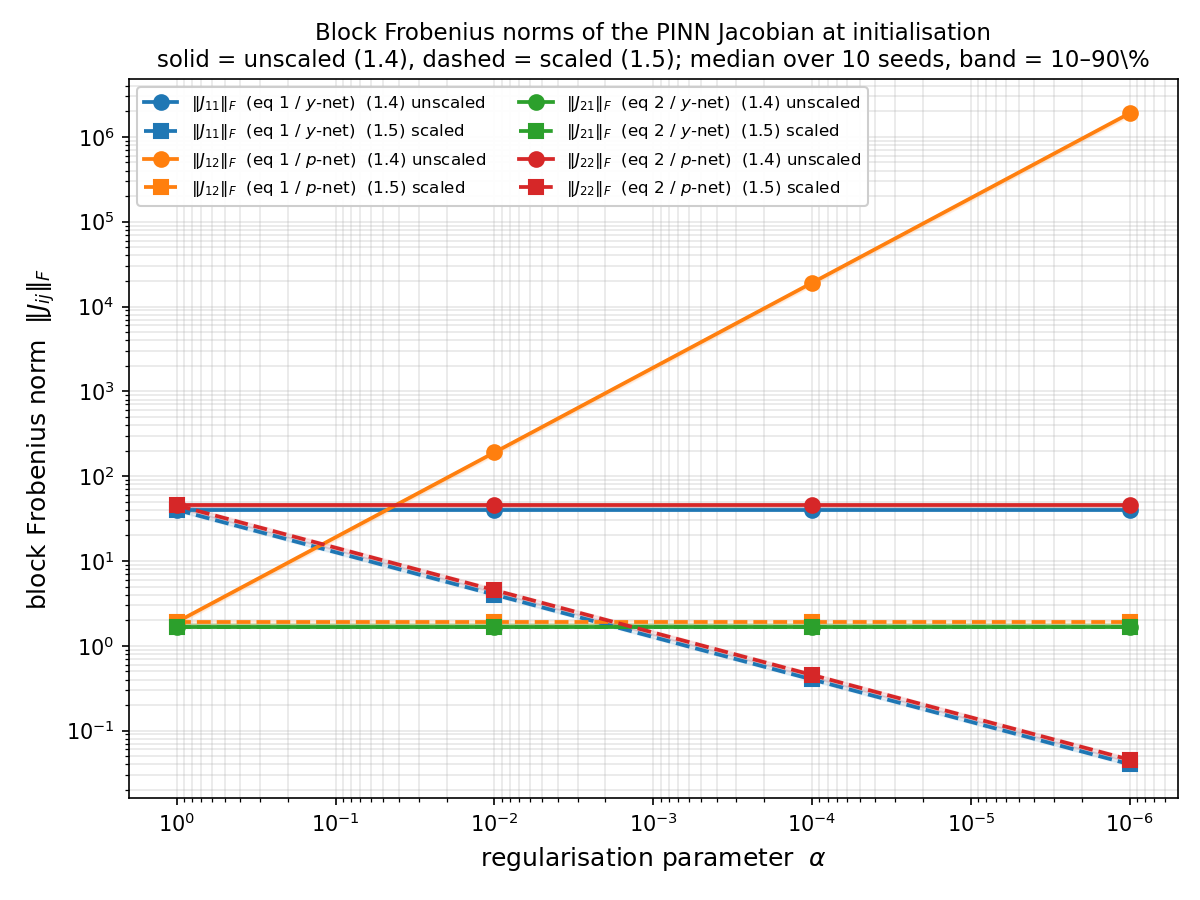
\includegraphics[width=0.86\linewidth]{exp0_fig_a_block_norms.png}
  \caption{PINN 雅可比四个子块的 Frobenius 范数随 $\alpha$ 变化
  （初始化时刻；$10$ 个随机种子的中位数）。
  实线为未缩放系统 (2.17)，虚线为缩放系统 (2.19)。
  未缩放 $\|J_{12}\|_F$ 随 $\alpha^{-1}$ 增长六个数量级；
  缩放系统所有块均 $\alpha$-有界。}
  \label{fig:block-norms}
\end{figure}

块级失衡传导至谱层面。图~\ref{fig:sigma-max} 给出 $\sigma_{\max}(J)$
的幂律：未缩放拟合斜率 $-0.80$（理论 $-1$），缩放拟合斜率 $+0.22$
（理论 $0$）；缩放系统的 Lipschitz 常数在整个扫描范围内保持
$\sigma_{\max}(J)\le 40$。

\begin{figure}[H]
  \centering
  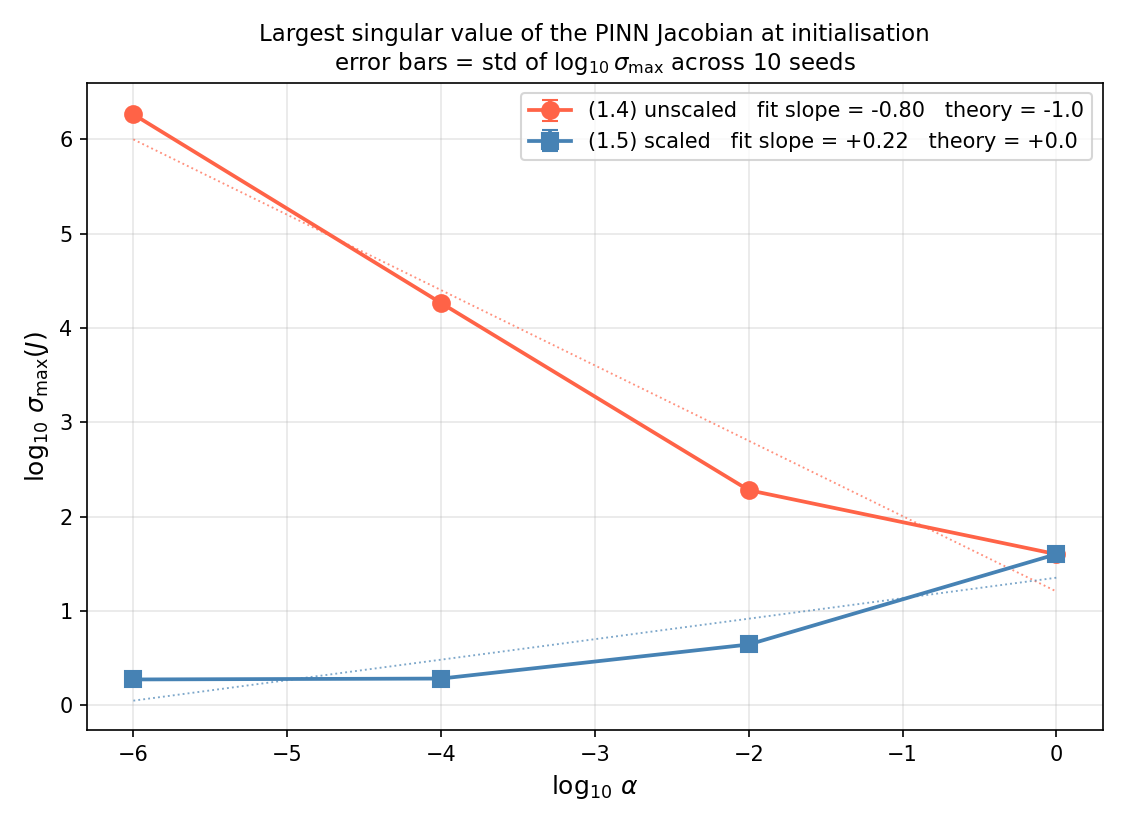
\includegraphics[width=0.70\linewidth]{exp0_fig_b_sigma_max.png}
  \caption{PINN 雅可比最大奇异值 $\sigma_{\max}(J)$ 在初始化时刻随 $\alpha$
  变化。未缩放拟合斜率 $-0.80$ 与理论 $-1$ 一致；
  缩放拟合斜率 $+0.22$，实质上 $\alpha$-独立。}
  \label{fig:sigma-max}
\end{figure}

\begin{remark}[关于条件数 $\kappa(J)$]
理论上 $\kappa(J) = \sigma_{\max}/\sigma_{\min}$ 可直接度量病态，
但深度网络雅可比上 $\sigma_{\min}$ 远低于 float64 精度下界，
其数值在整个扫描范围内稳定在 $10^{30}$ 量级附近——这是浮点精度伪影，
并不反映真实病态。以 $\sigma_{\max}$ 作为 Lipschitz 常数代理，
足以表达失衡的\emph{上侧}：Scaling 将 $\sigma_{\max}$ 从
$O(\alpha^{-1})$ 压到 $O(1)$。
\end{remark}

将块级失衡投影到参数空间即得梯度比率（图~\ref{fig:rho-init}）。
未缩放系统 $\log_{10}\rho$ 对 $\log_{10}\alpha$ 拟合斜率为 $-1.35$；
缩放系统斜率 $+0.22$，$\rho$ 始终在平衡点 $\rho = 1$ 附近。
拟合斜率稍陡于理论 $-1$ 的原因是：损失
$\mathcal L_k = \tfrac12\|r_k\|^2$ 对残差二次，$\alpha^{-1}$ 因子
在残差模长与雅可比行向量中各出现一次，于梯度模中复合。

\begin{figure}[H]
  \centering
  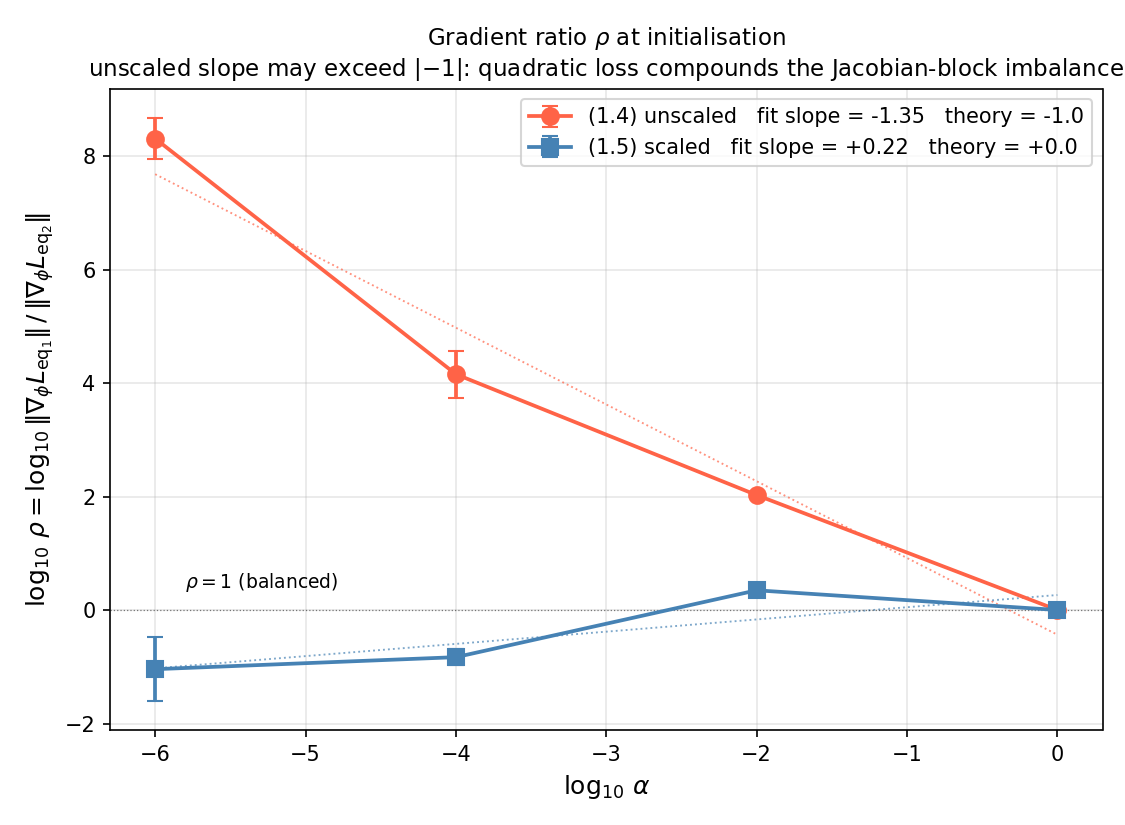
\includegraphics[width=0.70\linewidth]{exp0_fig_c_rho.png}
  \caption{初始化时的梯度比率 $\rho$。未缩放系统
  $\rho \sim \alpha^{-1}$（拟合斜率 $-1.35$）；
  缩放系统 $\rho \sim O(1)$（拟合斜率 $+0.22$）。
  $\rho = 1$ 虚线为完美平衡。}
  \label{fig:rho-init}
\end{figure}

% ------------------------------------------------------------------
\xmusubsection{训练过程中的梯度流}{Gradient flow during training}
\label{subsubsec:training-dynamics}

初始化时刻的结果不能排除训练动态自行消除失衡的可能。
图~\ref{fig:rho-training} 追踪 $\rho$ 贯穿 $5\,000$ 步训练的演化：
未缩放系统在任何 $\alpha\le 10^{-2}$ 下，$\rho$ 始终停留在初始量级
$\sim\alpha^{-1}$，训练动态\emph{没有}修复失衡；
缩放系统中 $\rho$ 全程维持在 $\rho = 1$ 附近，与 $\alpha$ 无关。

\begin{figure}[H]
  \centering
  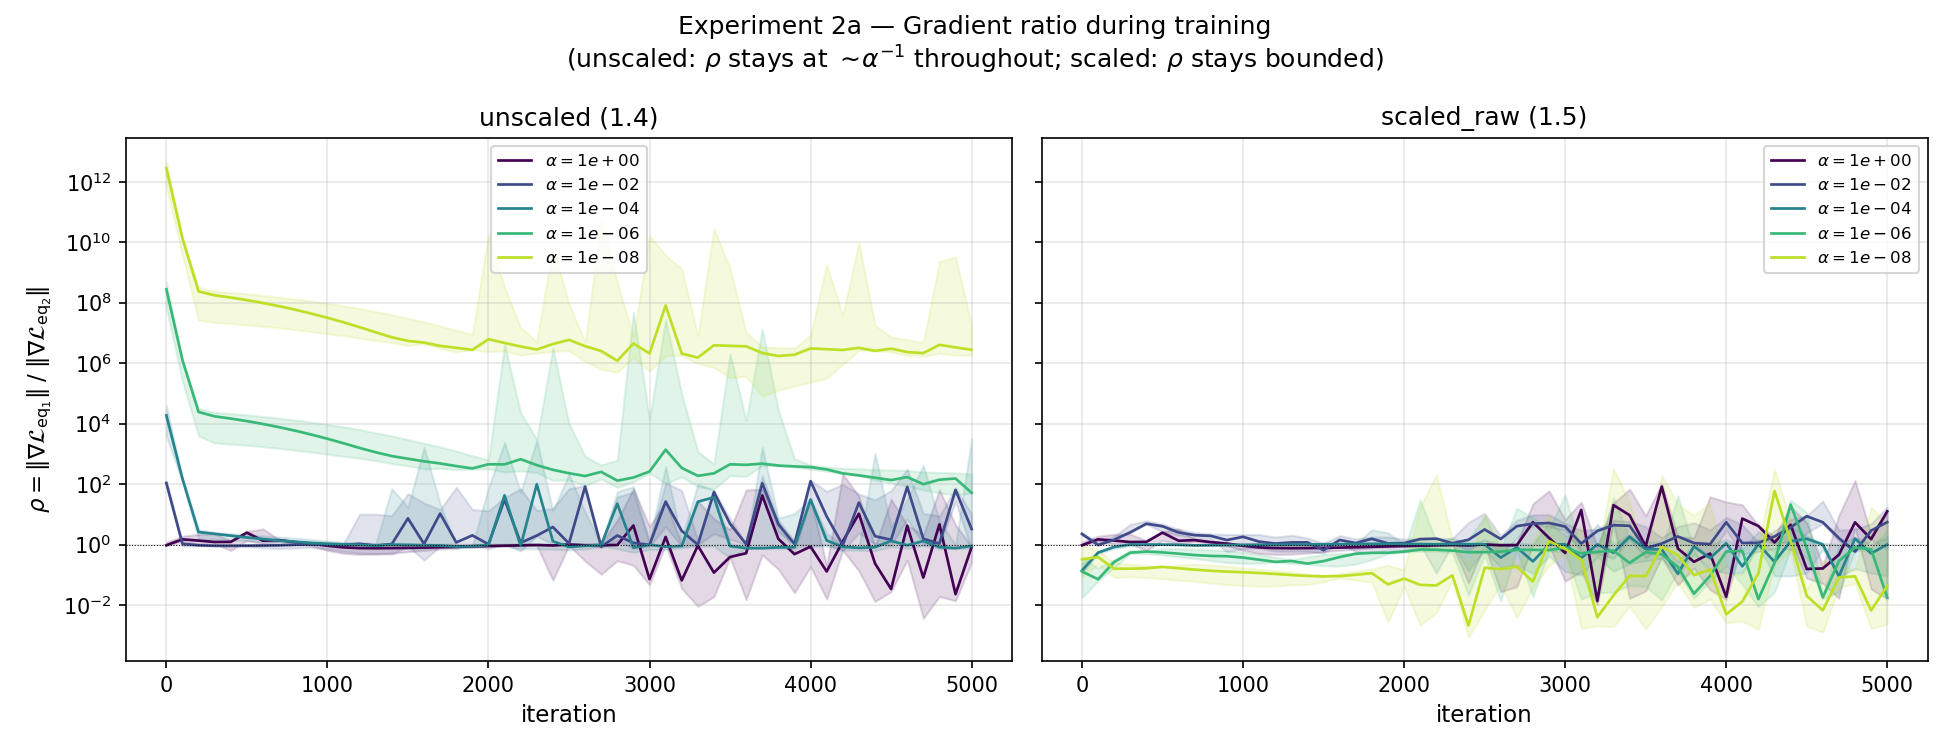
\includegraphics[width=\linewidth]{exp2_rho_training.png}
  \caption{梯度比率 $\rho$ 在训练全程的演化。
  未缩放（左）曲线随 $\alpha$ 减小整体上移而不衰减；
  缩放（右）所有 $\alpha$ 曲线塌缩到 $\rho = 1$ 附近。
  实线为 $3$ 个种子中位数，阴影为 $10$--$90\%$ 分位区间。}
  \label{fig:rho-training}
\end{figure}



% ------------------------------------------------------------------
\xmusubsection{$\rho$--$\omega$ 关系：原理层与现象层的桥梁}%
{The $\rho$--$\omega$ relation: bridging principle and phenomenon}
\label{subsubsec:rho-omega}

§\ref{subsubsec:omega-sweep} 将观察到的 $\omega$-鲁棒性，可由 $\rho$
对损失权重的依赖直接解释。令损失为
$\mathcal L = \omega \mathcal L_{\mathrm{eq}_1} + \mathcal L_{\mathrm{eq}_2}$，
则 $\rho_\omega = \omega\cdot\rho_0(\alpha)$，即
$\log_{10}\rho_\omega = \log_{10}\omega + \log_{10}\rho_0(\alpha)$：
斜率为 $+1$，\emph{截距}由 $\alpha$-病态决定。

图~\ref{fig:rho-omega}~(a) 确认两侧斜率均为 $+1$。
图~\ref{fig:rho-omega}~(b) 给出\emph{距平衡的距离}
$|\log_{10}\rho_\omega|$：缩放系统在 $\omega\in[1,10]$ 内极度接近
$|\log\rho| = 0$，存在宽阔的"平衡走廊"；
未缩放系统在扫描范围 $\omega\in[10^{-2}, 10^2]$ 内任一点都
距平衡 $\ge 2$ 个数量级——纯粹调整 $\omega$ 无法把未缩放系统推回平衡。
这就是现象层 \emph{Scaling 鲁棒、Unscaled 脆弱} 的原理层证据。

\begin{figure}[H]
  \centering
  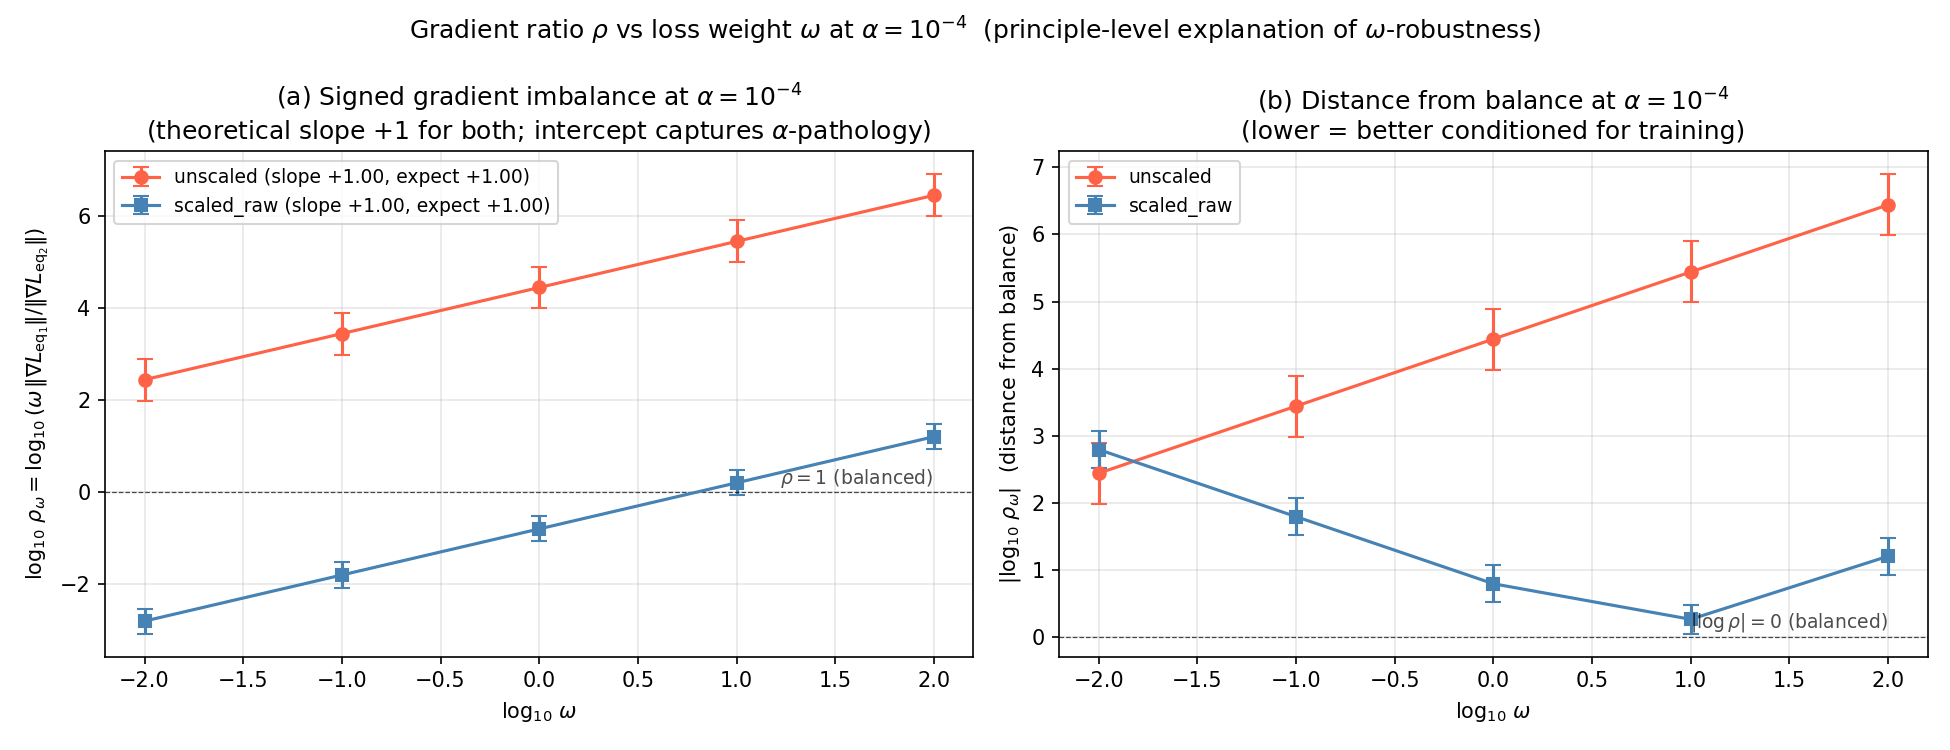
\includegraphics[width=\linewidth]{exp_rho_vs_omega.png}
  \caption{固定 $\alpha = 10^{-4}$ 时梯度比率 $\rho_\omega$ 对损失权重
  $\omega$ 的依赖。(a) 线性拟合，两侧斜率均为 $+1$，截距相差 $\sim 4$
  个数量级；(b) $|\log_{10}\rho_\omega|$ 距平衡距离——缩放系统在
  $\omega\in[1,10]$ 接近平衡，未缩放系统在全部扫描范围内都远离平衡。}
  \label{fig:rho-omega}
\end{figure}

\begin{remark}
§\ref{subsubsec:jacobian}--\ref{subsubsec:rho-omega} 合起来给出一条
闭合的证据链：块级失衡 $\Rightarrow$ 谱级失衡 $\Rightarrow$ 参数空间失衡
$\Rightarrow$ 该失衡贯穿整个训练 $\Rightarrow$ $\omega$ 仅能沿对数轴
平移、无法消除。此五维证据全部独立于误差指标；
下节 §\ref{subsec:phenomenon} 的误差表格只是该结构性结论在外部度量
上的反映。
\end{remark}

% ==================================================================

\xmusection{现象层：对外部扰动的鲁棒性}{Phenomenon-level Robustness}
\label{subsec:phenomenon}

本节在原理层证据之上，用误差指标验证 Scaling 对两种外部扰动
——正则化参数 $\alpha$ 与损失权重 $\omega$——的鲁棒性。
主体实验固定在 Hard BC + Dual Network 的\emph{标准设置}，
以排除软边界与参数共享带来的混杂因素；
Soft BC 下的适用范围界定见 §\ref{subsubsec:softbc}。

% ------------------------------------------------------------------
\xmusubsection{$\alpha$-扫描}{$\alpha$-sweep}
\label{subsubsec:alpha-sweep}

固定等权重 $\gamma = 1$，扫描
$\alpha\in\{10^{-2},10^{-3},10^{-4},10^{-5}\}$。
结果见表~\ref{tab:alpha-hard-dual} 与图~\ref{fig:alpha-hard-dual}。

\begin{table}[H]
  \centering
  \caption{$\alpha$-敏感性：Hard BC + Dual Network，$\gamma = 1$}
  \label{tab:alpha-hard-dual}
  \small
  \begin{tabular}{cc rrrr}
  \toprule
  $\alpha$ & 系统 & $L^2_y$ & $L^2_p$ & $H^1_y$ & $H^1_p$ \\
  \midrule
  \multirow{2}{*}{$10^{-2}$}
  & Unscaled & $5.77\times10^{-5}$ & $4.64\times10^{-3}$ & $1.11\times10^{-4}$ & $8.92\times10^{-3}$ \\
  & Scaled   & $4.81\times10^{-5}$ & $3.33\times10^{-3}$ & $9.66\times10^{-5}$ & $6.77\times10^{-3}$ \\
  \midrule
  \multirow{2}{*}{$10^{-3}$}
  & Unscaled & $4.34\times10^{-4}$ & $2.74\times10^{-2}$ & $6.95\times10^{-4}$ & $5.54\times10^{-2}$ \\
  & Scaled   & $6.66\times10^{-4}$ & $4.14\times10^{-2}$ & $1.11\times10^{-3}$ & $8.10\times10^{-2}$ \\
  \midrule
  \multirow{2}{*}{$10^{-4}$}
  & Unscaled & $1.09\times10^{-2}$ & $7.32\times10^{-1}$ & $1.98\times10^{-2}$ & $1.51\times10^{+0}$ \\
  & Scaled   & $9.43\times10^{-4}$ & $6.72\times10^{-2}$ & $1.74\times10^{-3}$ & $1.42\times10^{-1}$ \\
  \midrule
  \multirow{2}{*}{$10^{-5}$}
  & Unscaled & $\mathbf{1.00\times10^{+0}}$ & $\mathbf{1.22\times10^{+1}}$
             & $\mathbf{1.00\times10^{+0}}$ & $\mathbf{1.22\times10^{+1}}$ \\
  & Scaled   & $1.92\times10^{-3}$ & $1.24\times10^{-1}$ & $3.30\times10^{-3}$ & $2.32\times10^{-1}$ \\
  \bottomrule
  \end{tabular}
\end{table}

\begin{figure}[H]
  \centering
  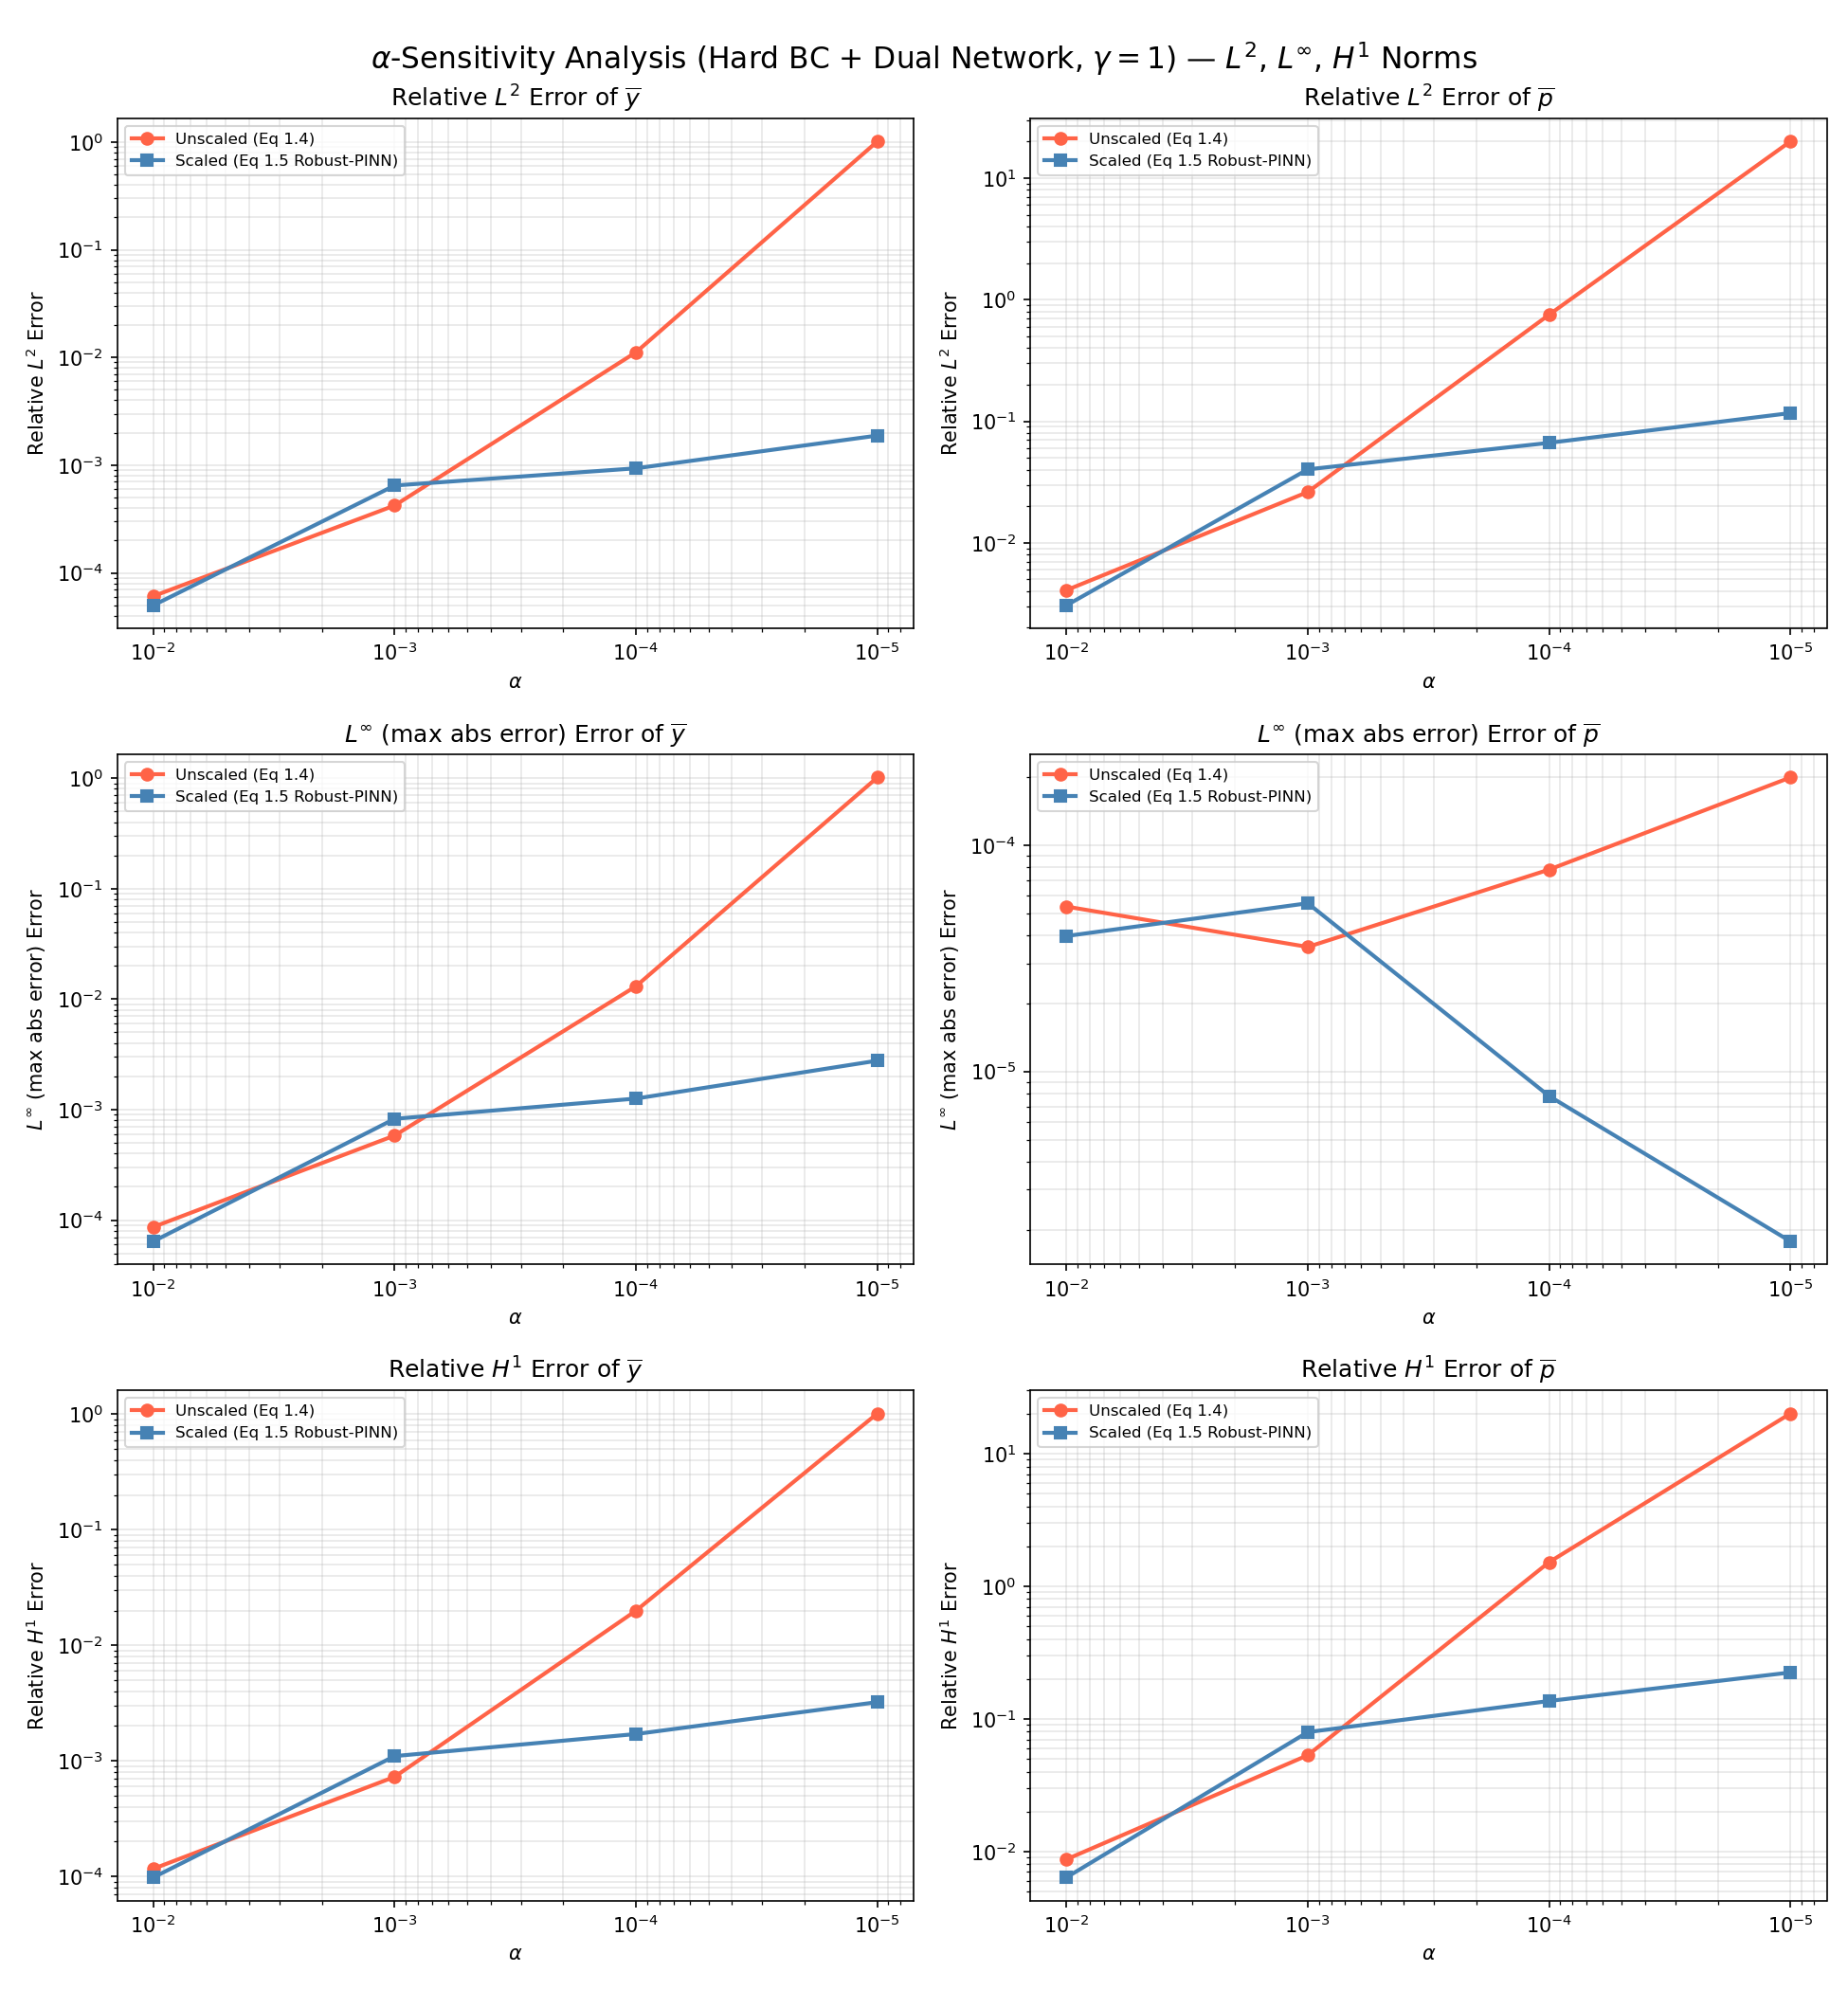
\includegraphics[width=\linewidth]{alpha_test_hardBC_dualnet_result.png}
  \caption{$\alpha$-敏感性（Hard BC + Dual Network，$\gamma = 1$）。
  未缩放曲线在 $\alpha\le 10^{-4}$ 附近出现"剪刀式"发散，
  $\alpha = 10^{-5}$ 时 $L^2_y\to 1$——网络退化为平凡解
  （详见 §\ref{subsec:forensics}）；缩放曲线在全 $\alpha$ 范围内近乎水平。}
  \label{fig:alpha-hard-dual}
\end{figure}



% ------------------------------------------------------------------
\xmusubsection{$\omega$-扫描}{$\omega$-sweep}
\label{subsubsec:omega-sweep}

固定 $\alpha = 10^{-4}$（§\ref{subsubsec:alpha-sweep} 已显示该值下
Unscaled 进入失效区），将损失设为
$\gamma \mathcal L_{\mathrm{eq}_1} + \mathcal L_{\mathrm{eq}_2}$，
扫描 $\gamma\in\{10^{-2},10^{-1},1,10,10^2\}$。

\begin{table}[H]
  \centering
  \caption{$\omega$-敏感性：Hard BC + Dual Network，$\alpha = 10^{-4}$}
  \label{tab:omega-hard-dual}
  \small
  \begin{tabular}{cc rrrr}
  \toprule
  $\gamma$ & 系统 & $L^2_y$ & $L^2_p$ & $H^1_y$ & $H^1_p$ \\
  \midrule
  \multirow{2}{*}{$0.01$}
  & Unscaled & $3.46\times10^{-3}$ & $2.49\times10^{-1}$ & $6.91\times10^{-3}$ & $5.39\times10^{-1}$ \\
  & Scaled   & $1.67\times10^{-3}$ & $9.49\times10^{-2}$ & $2.70\times10^{-3}$ & $1.69\times10^{-1}$ \\
  \midrule
  \multirow{2}{*}{$0.1$}
  & Unscaled & $3.74\times10^{-3}$ & $2.96\times10^{-1}$ & $7.29\times10^{-3}$ & $6.45\times10^{-1}$ \\
  & Scaled   & $7.48\times10^{-4}$ & $6.28\times10^{-2}$ & $1.50\times10^{-3}$ & $1.39\times10^{-1}$ \\
  \midrule
  \multirow{2}{*}{$1$}
  & Unscaled & $1.82\times10^{-2}$ & $7.65\times10^{-1}$ & $2.37\times10^{-2}$ & $1.48\times10^{+0}$ \\
  & Scaled   & $1.04\times10^{-3}$ & $7.21\times10^{-2}$ & $1.88\times10^{-3}$ & $1.47\times10^{-1}$ \\
  \midrule
  \multirow{2}{*}{$10$}
  & Unscaled & $\mathbf{9.84\times10^{-1}}$ & $\mathbf{1.94\times10^{+1}}$
             & $\mathbf{9.84\times10^{-1}}$ & $\mathbf{1.94\times10^{+1}}$ \\
  & Scaled   & $1.38\times10^{-3}$ & $7.04\times10^{-2}$ & $2.17\times10^{-3}$ & $1.18\times10^{-1}$ \\
  \midrule
  \multirow{2}{*}{$100$}
  & Unscaled & $\mathbf{9.90\times10^{-1}}$ & $\mathbf{1.95\times10^{+1}}$
             & $\mathbf{9.90\times10^{-1}}$ & $\mathbf{1.95\times10^{+1}}$ \\
  & Scaled   & $6.67\times10^{-3}$ & $1.84\times10^{-1}$ & $7.44\times10^{-3}$ & $2.62\times10^{-1}$ \\
  \bottomrule
  \end{tabular}
\end{table}

\begin{figure}[H]
  \centering
  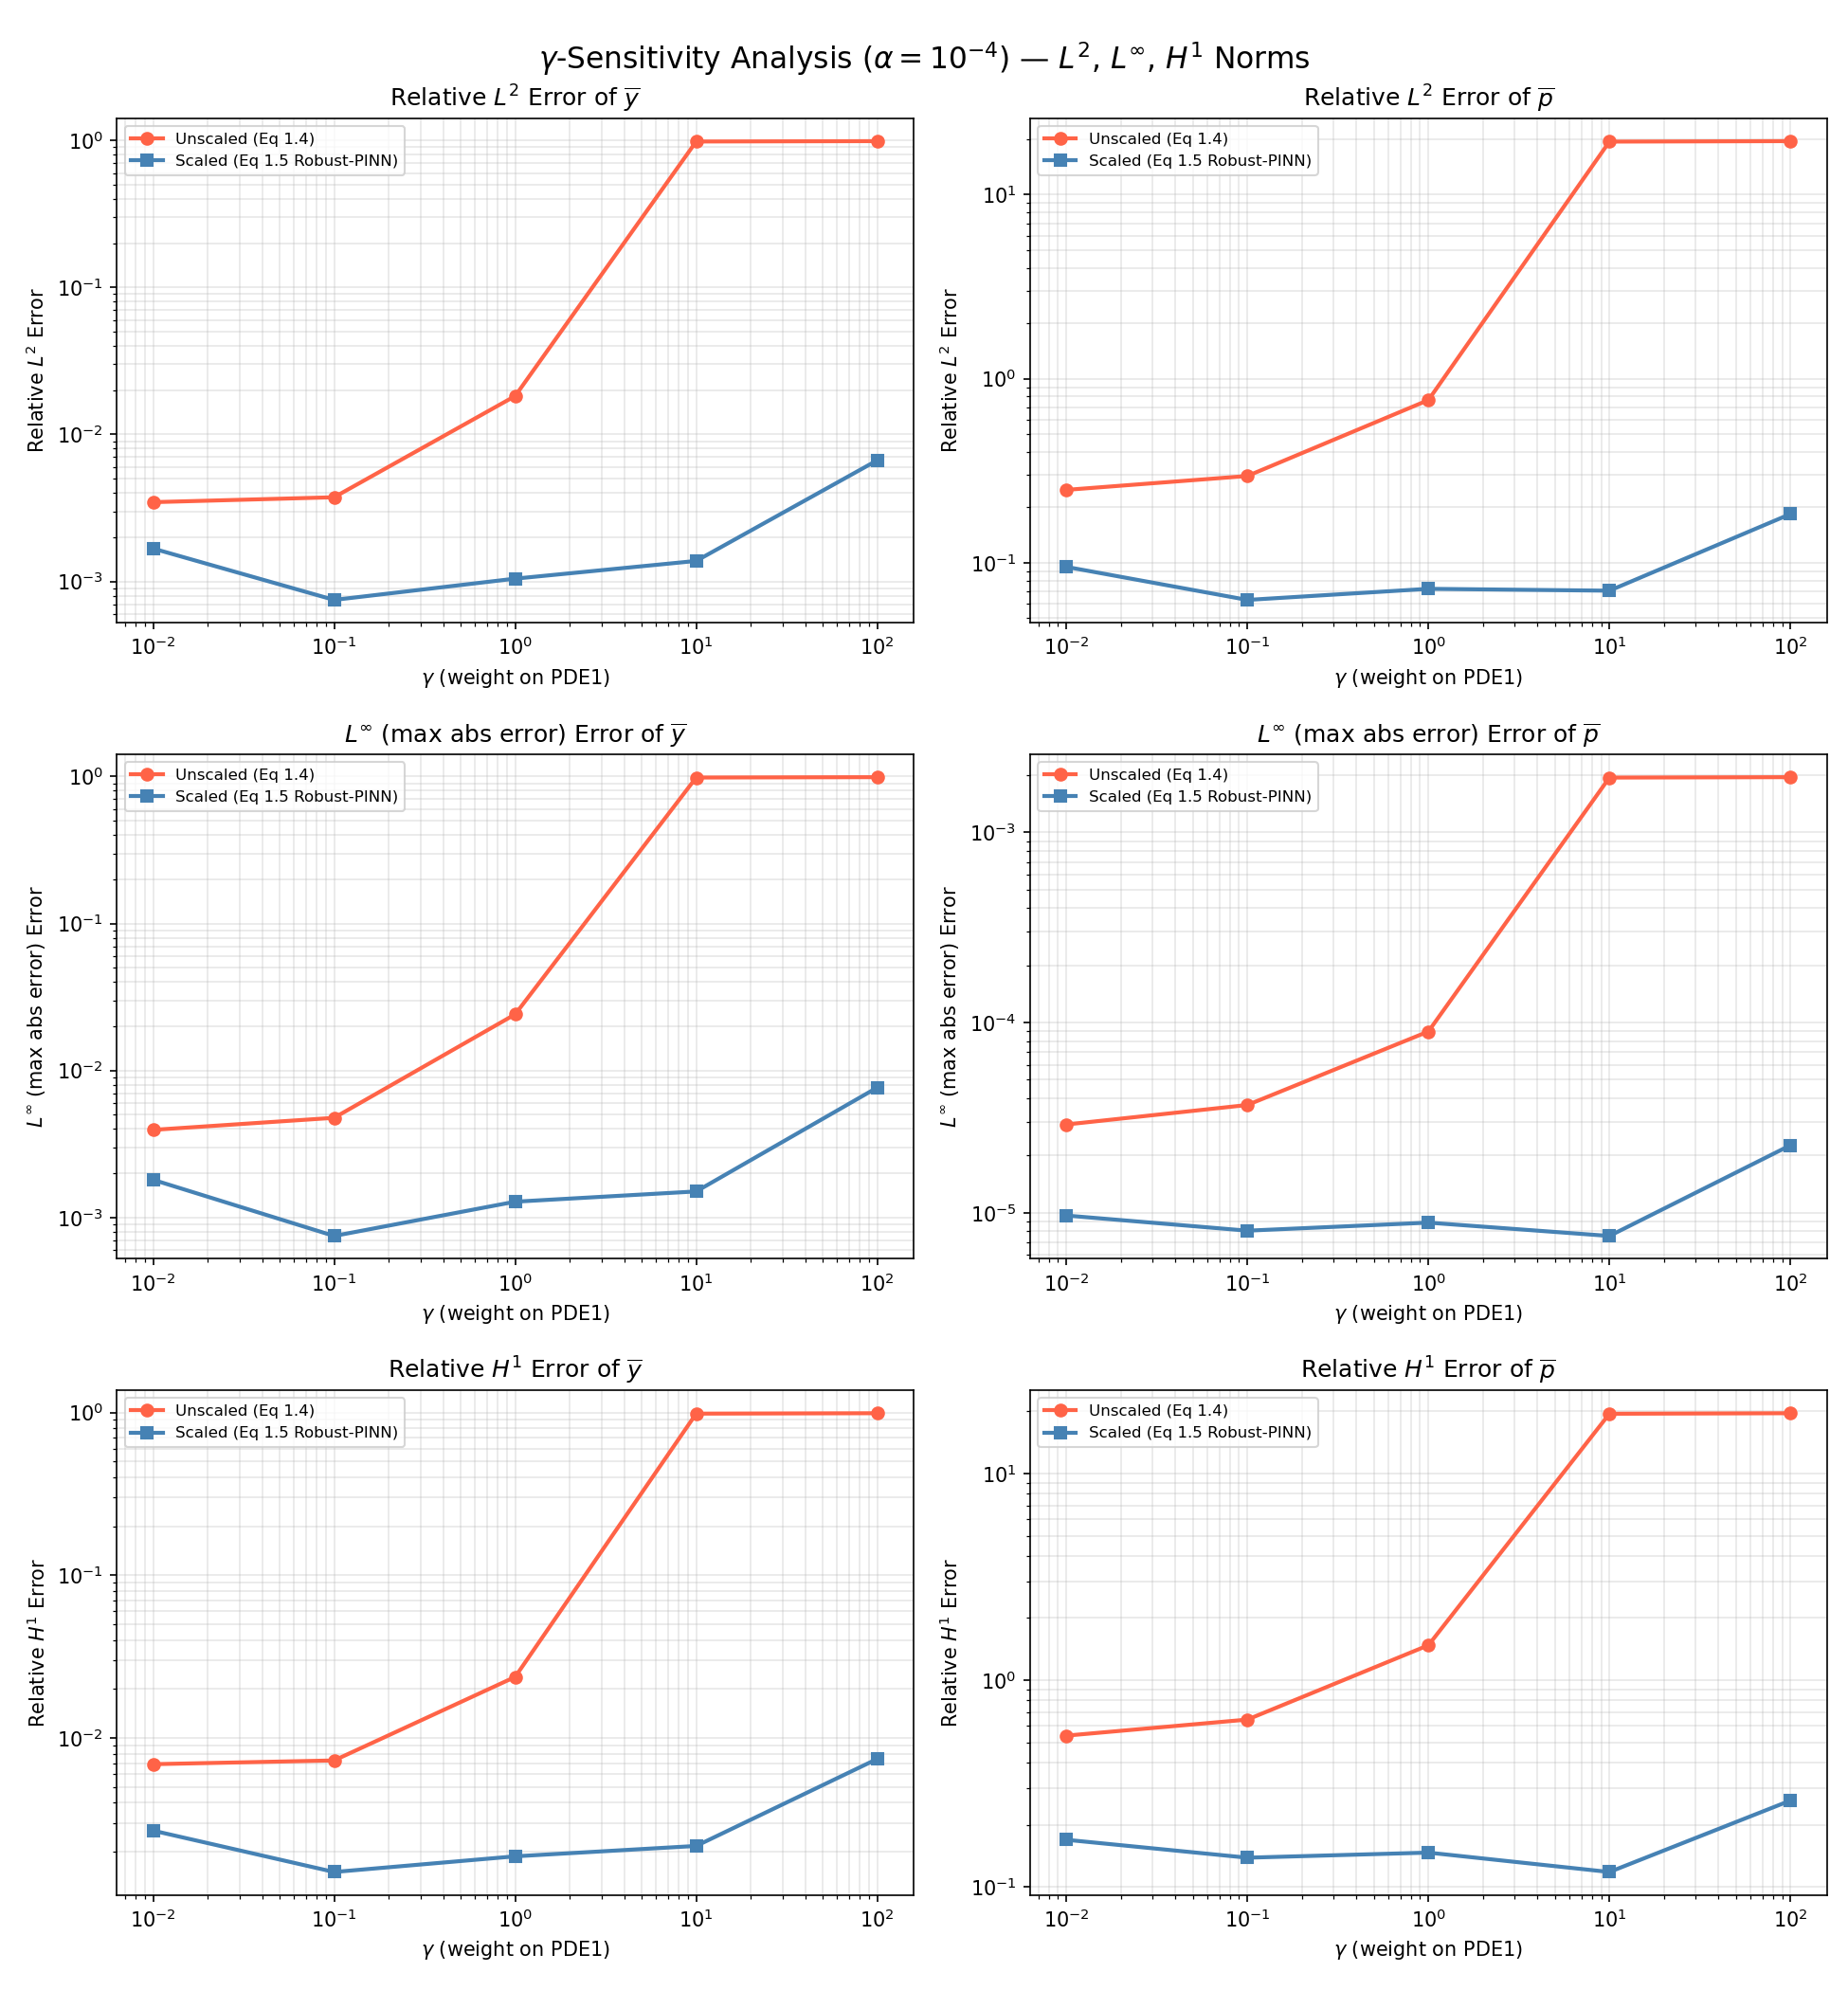
\includegraphics[width=\linewidth]{weight_sensitivity_result.png}
  \caption{$\omega$-敏感性（Hard BC + Dual Network，$\alpha = 10^{-4}$）：
  相对 $L^2$、$L^\infty$、$H^1$ 误差随 $\gamma$ 的变化。未缩放系统
  可用的权重窗口极窄（$\gamma\le 1$ 尚可，$\gamma\ge 10$ 完全崩溃）；
  缩放系统跨 $4$ 个数量级稳定在 $L^2_y\sim 10^{-3}$。}
  \label{fig:omega-hard-dual}
\end{figure}

此处的观察与 §\ref{subsubsec:rho-omega} 的理论预测定量吻合：
未缩放系统 $\rho_\omega$ 在 $\gamma\in[10^{-2},10^2]$ 内距离平衡
$\ge 2$ 个数量级，故任何 $\gamma$ 取值都无法恢复平衡；
缩放系统的"平衡走廊"落在 $\gamma\in[1,10]$，与误差指标的最佳区间
完全一致（表中 Scaled 在 $\gamma\in\{0.1,1,10\}$ 均给出 $L^2_y\sim 10^{-3}$）。

% ------------------------------------------------------------------
\xmusubsection{Soft BC 下的适用范围界定}{Scope under Soft BC}
\label{subsubsec:softbc}

实际几何复杂时须使用 Soft BC，损失增至
\[
  \mathcal L = \mathcal L_{\mathrm{PDE}} + w_{bc}\,\mathcal L_{\mathrm{BC}}.
\]
Scaling 处理的是残差系统\emph{内部}（$\mathrm{eq}_1$ 与 $\mathrm{eq}_2$
之间）的失衡；PDE 与边界的\emph{跨类}失衡由 $w_{bc}$ 控制，
与 Scaling 正交——这解释了为何在 Soft BC 等权重
（$w_{bc} = 1$）情形下，两系统误差曲线近似平行而非呈现
Hard BC 下的剪刀型：$w_{bc} = 1$ 时边界残差主导整个损失，
两种不同的失衡叠加掩盖了 Scaling 的$\alpha$-鲁棒性。
为明确界定方法的有效范围，在 Soft BC + Dual Network 设置下对
$w_{bc}\in\{1,10,100,1000\}$ 与 $\alpha\in\{10^{-2},10^{-3},10^{-4},10^{-5}\}$
做二维扫描（图~\ref{fig:wbc-sweep}）。

\begin{figure}[H]
  \centering
  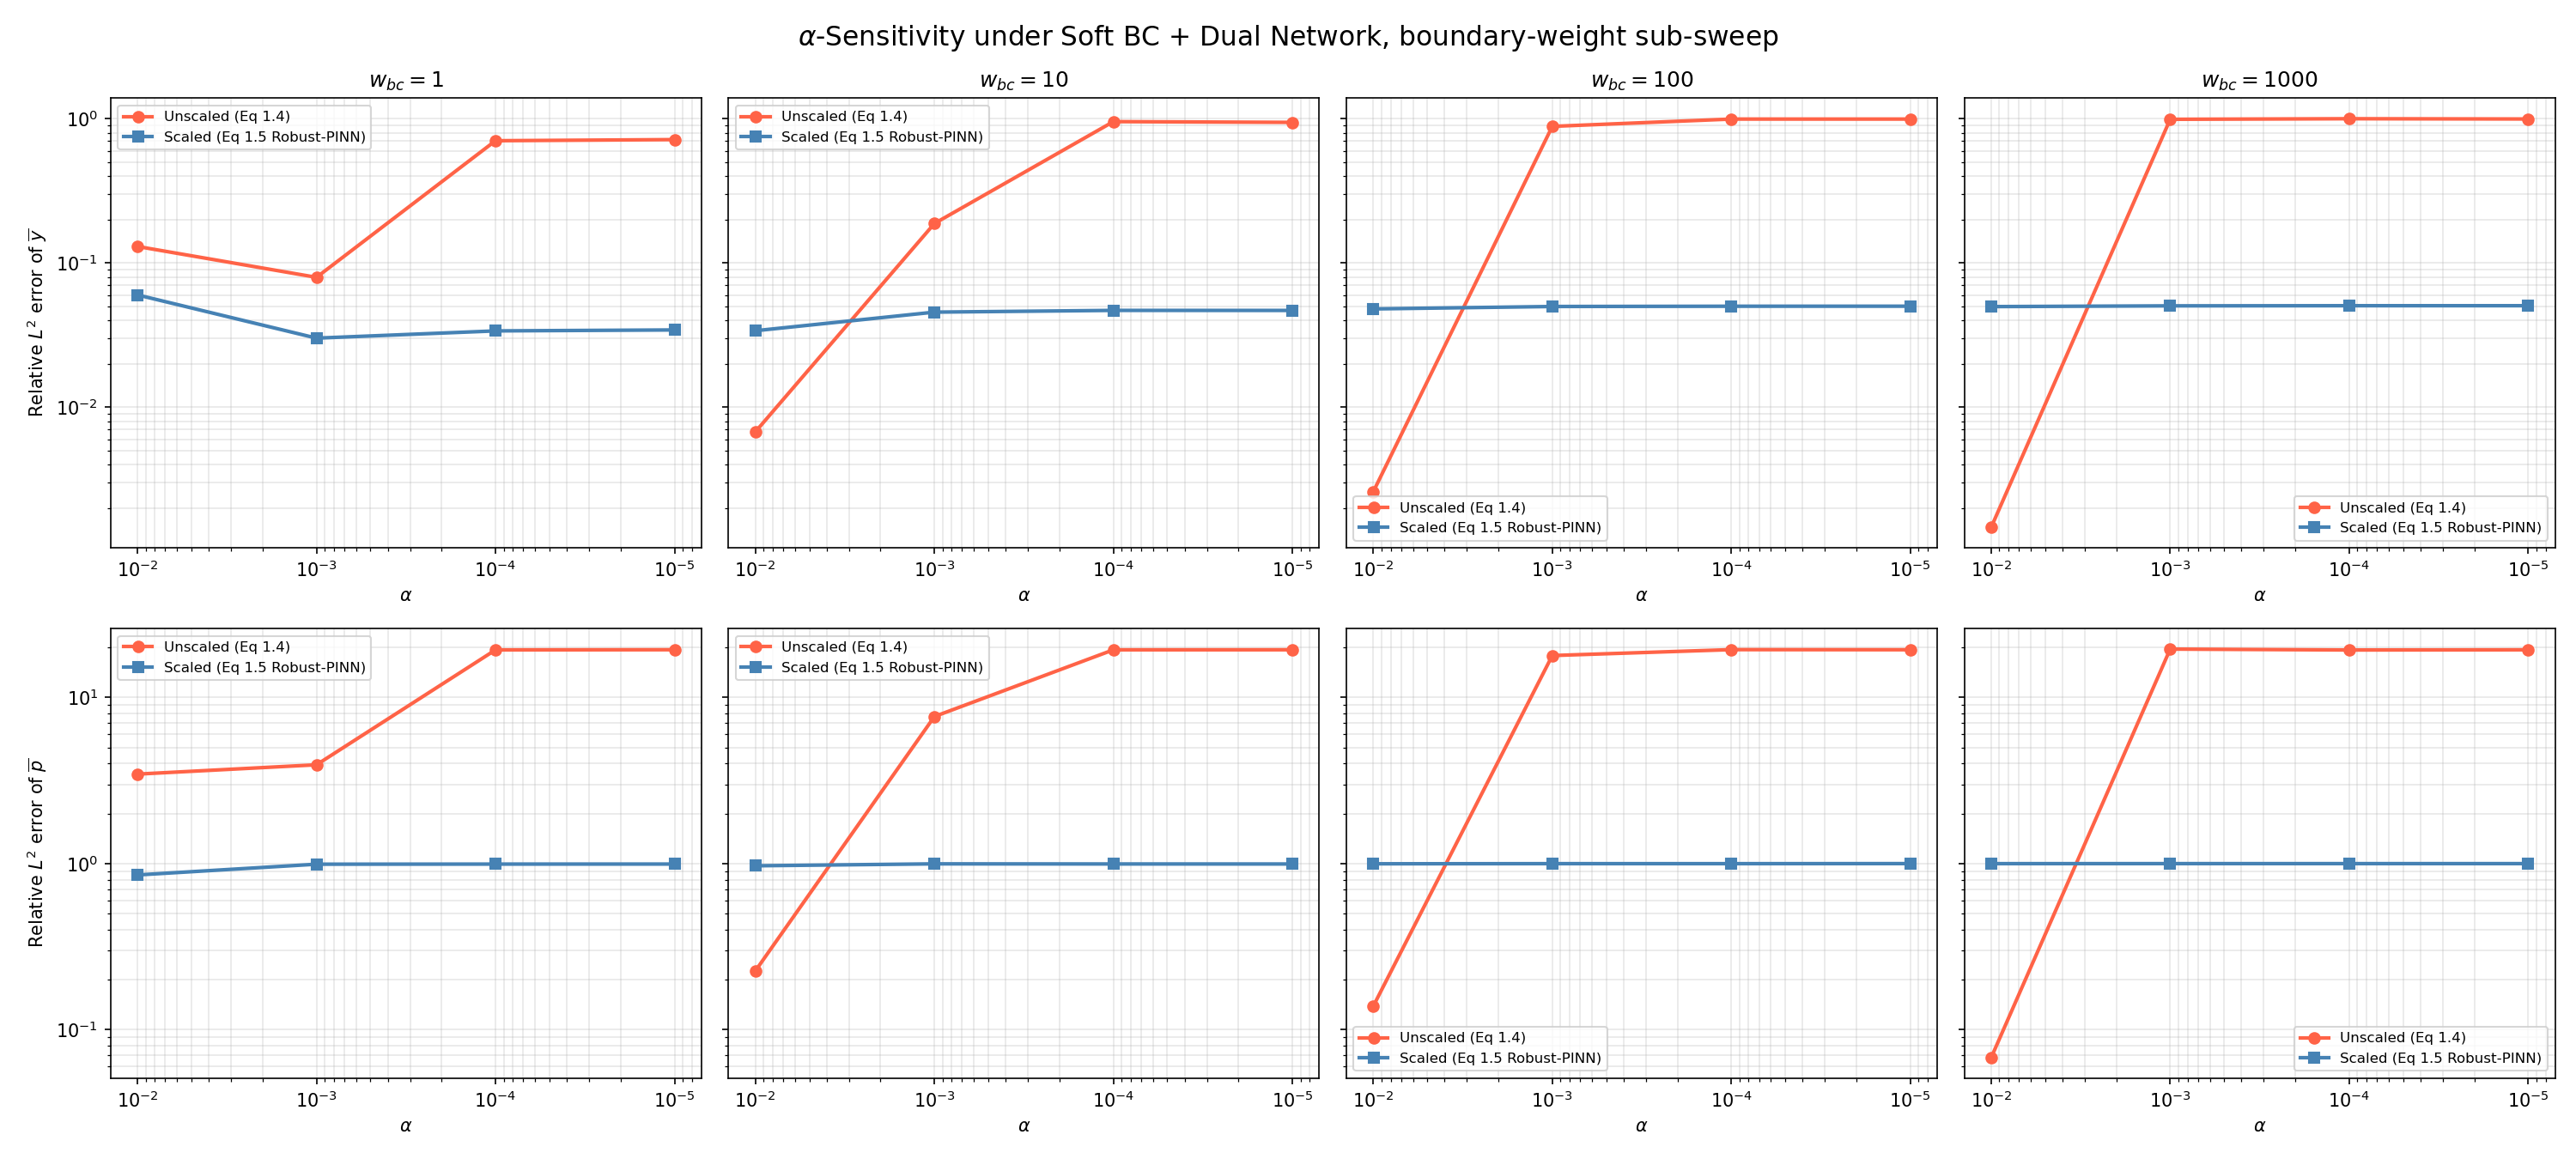
\includegraphics[width=\linewidth]{alpha_test_softBC_dualnet_wbc_sweep_result.png}
  \caption{Soft BC + Dual Network 下 $w_{bc}$ 与 $\alpha$ 的联合扫描。
  上排：$L^2_y$；下排：$L^2_p$；列为不同 $w_{bc}$。}
  \label{fig:wbc-sweep}
\end{figure}

对 $\bar y$：$w_{bc}\ge 10$ 下 Unscaled 在 $\alpha\le 10^{-4}$ 完全失效
（$L^2_y\to 1$），Scaled 稳定在 $L^2_y\approx 5\times 10^{-2}$；
即使 $w_{bc} = 1$ 的最不利情形，Scaled 仍比 Unscaled 好约一个数量级。

对 $\bar p$：Scaled 系统的相对 $L^2_p \approx 1$ 并非未学习，而是
\emph{分母伪影}——$\|\bar p_{\rm exact}\| = O(\alpha)$ 随 $\alpha$
急剧衰减，相对指标被小分母放大；绝对误差 $L^\infty_p$ 仍在 $O(10^{-6})$
量级（§\ref{subsec:forensics} 的可视化确证了这一点）。

\begin{remark}[适用范围声明]
Scaling 修复 KKT 系统的\emph{内部}失衡，是结构性改进；
它\emph{不}处理 PDE 与 BC 的\emph{跨类}失衡。
在 Hard BC 或 $w_{bc}\ge 10$ 的 Soft BC 下，方法达到设计目标；
$w_{bc} = 1$ 的等权 Soft BC 下两种失衡叠加，Scaling 的 $\alpha$-优势
部分被 BC-失效遮蔽，但在 $L^2_y$ 上仍保持可测量的数量级优势。
\end{remark}

% ==================================================================

\xmusection{失效模式剖析}{Failure-mode Forensics}
\label{subsec:forensics}

表~\ref{tab:alpha-hard-dual} 中 $\alpha = 10^{-5}$ 的 $L^2_y\approx 1$
仅是一个数字。为将失效机制具体化，我们选择直接加载该单元格训练得到的两个网络，
在 $100\times 100$ 网格上可视化（图~\ref{fig:forensic-y}、\ref{fig:forensic-p}）。
此处的网络权重与表~\ref{tab:alpha-hard-dual} 的训练检查点严格一致。

\begin{figure}[H]
  \centering
  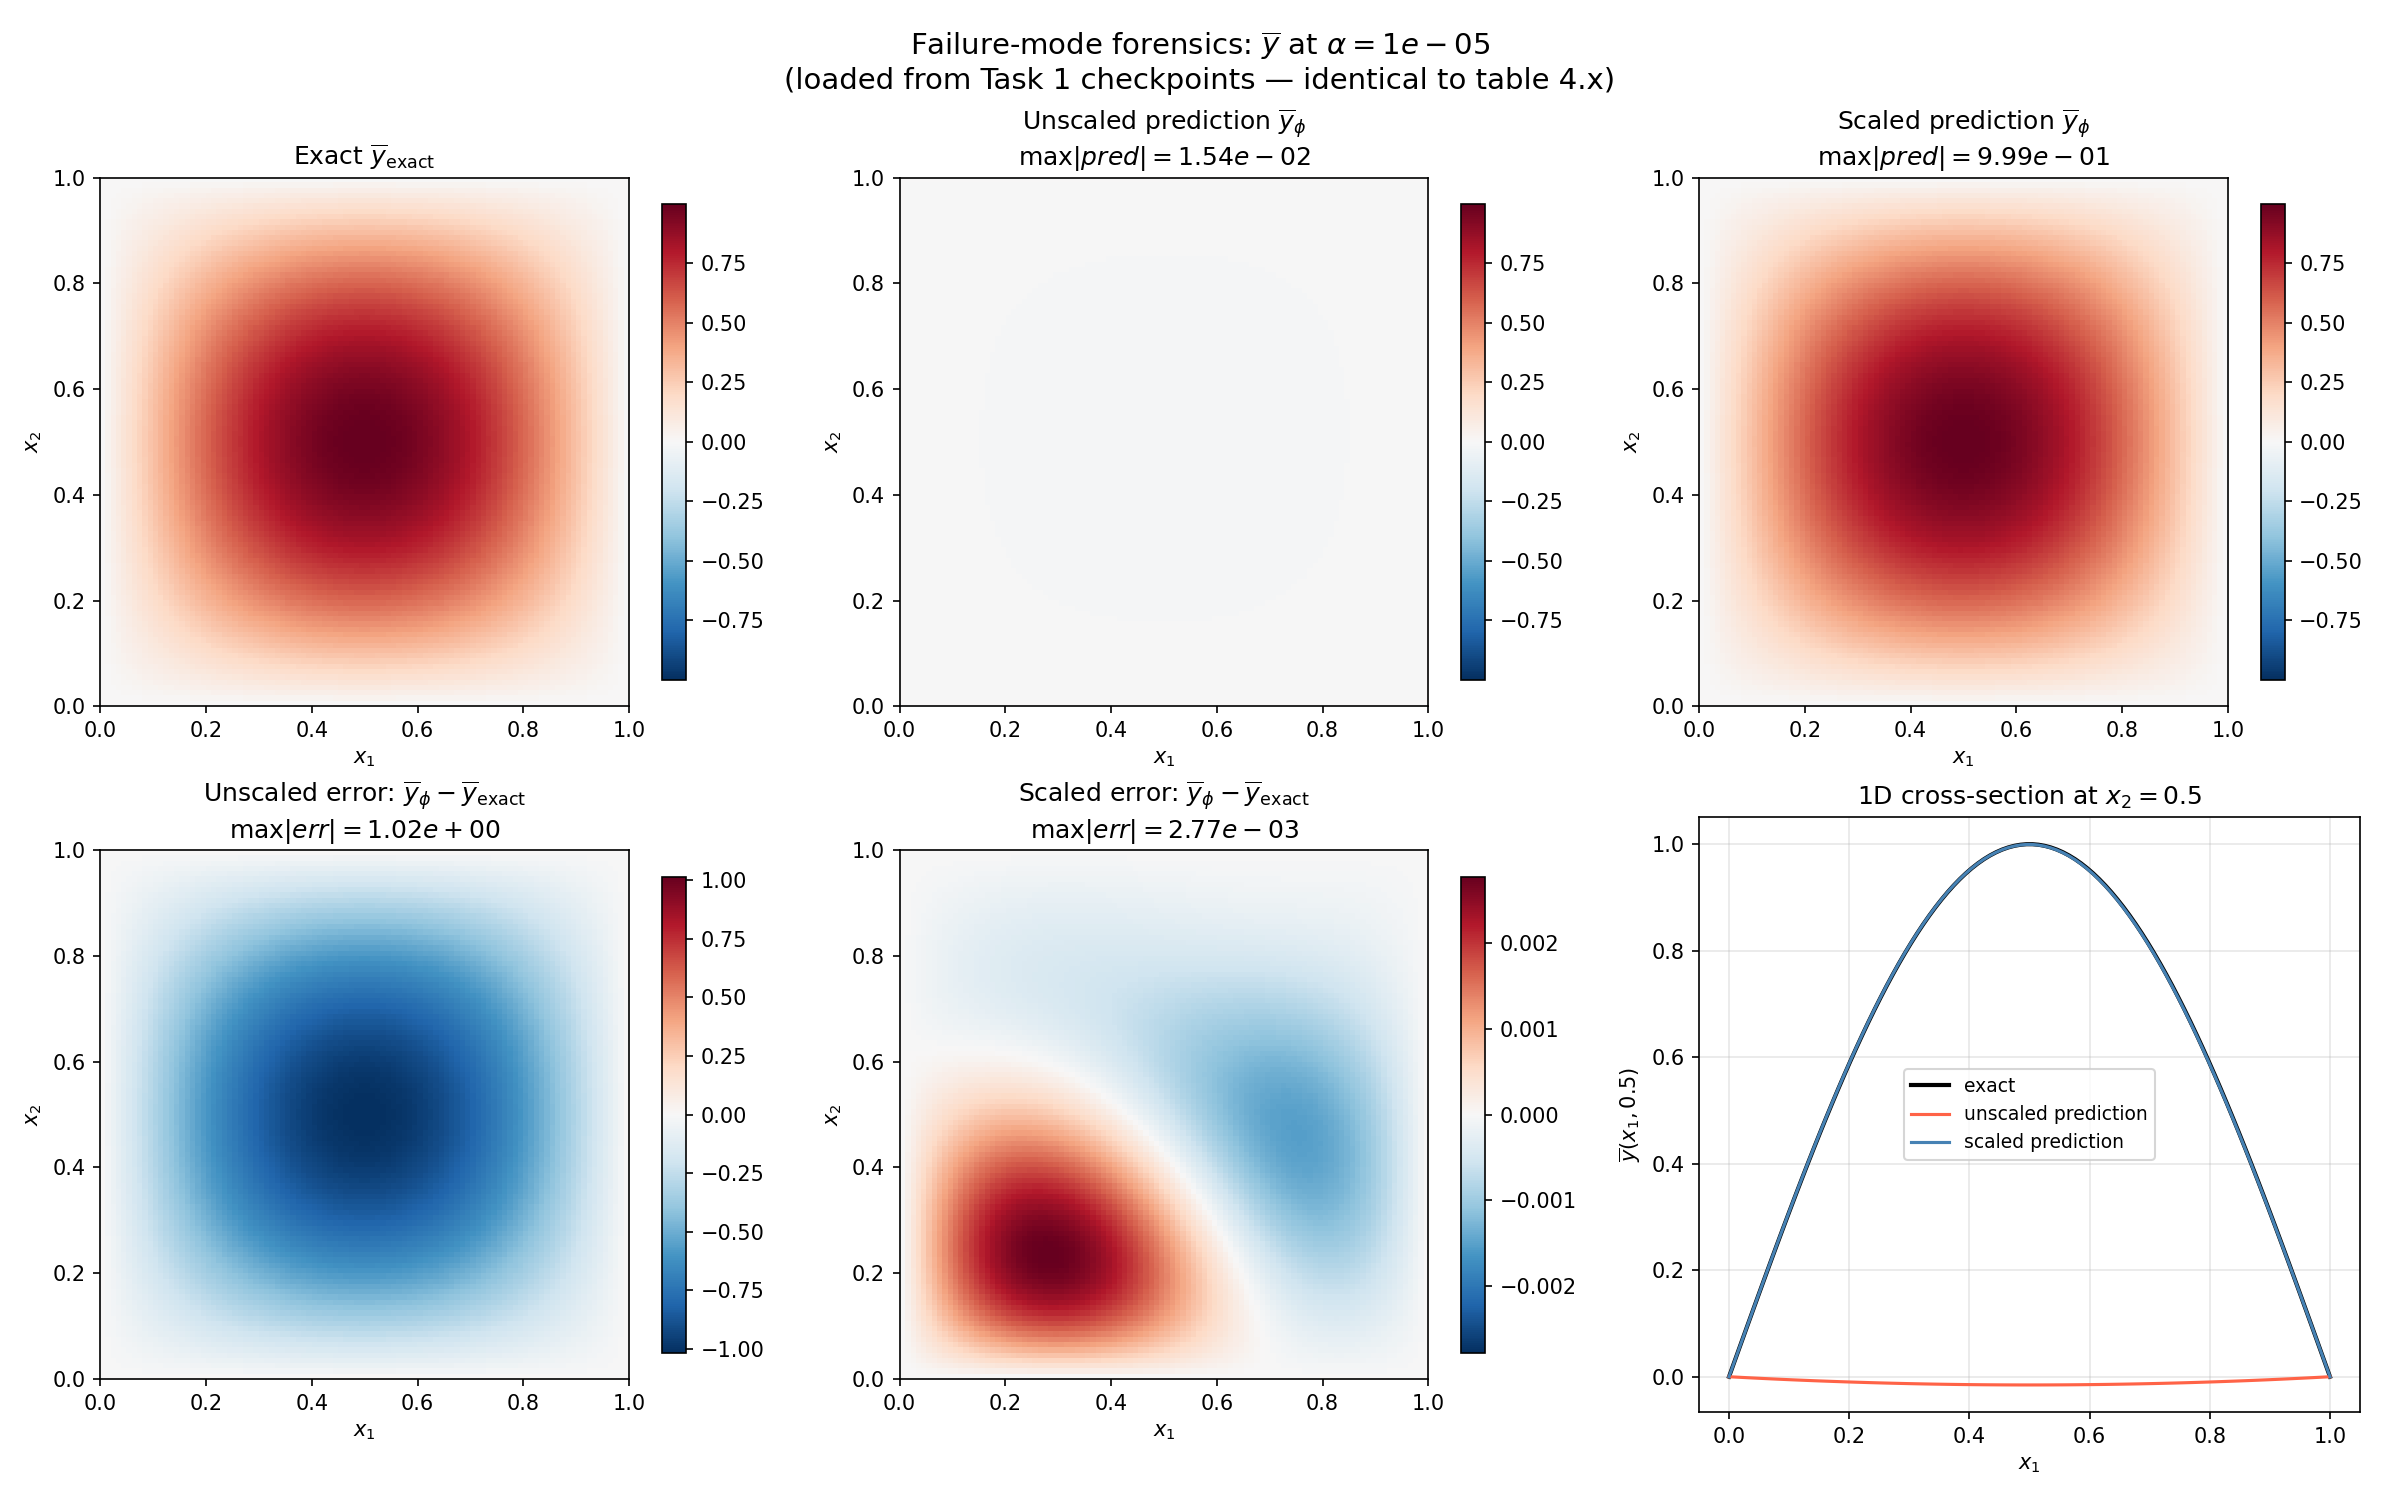
\includegraphics[width=\linewidth]{failure_mode_y.png}
  \caption{$\alpha = 10^{-5}$ 时状态变量 $\bar y$ 预测场的对比。
  Unscaled 网络最大预测值仅 $1.54\times 10^{-2}$——对
  $\max|\bar y_{\rm exact}| = 1$ 而言几乎退化至零；
  Scaled 网络 $\max|\bar y_\phi| = 0.999$，逐点误差 $\le 2.77\times 10^{-3}$。
  一维切片（右下）显示 Scaled 与精确解目视重合，Unscaled 几乎贴零。}
  \label{fig:forensic-y}
\end{figure}

\begin{figure}[H]
  \centering
  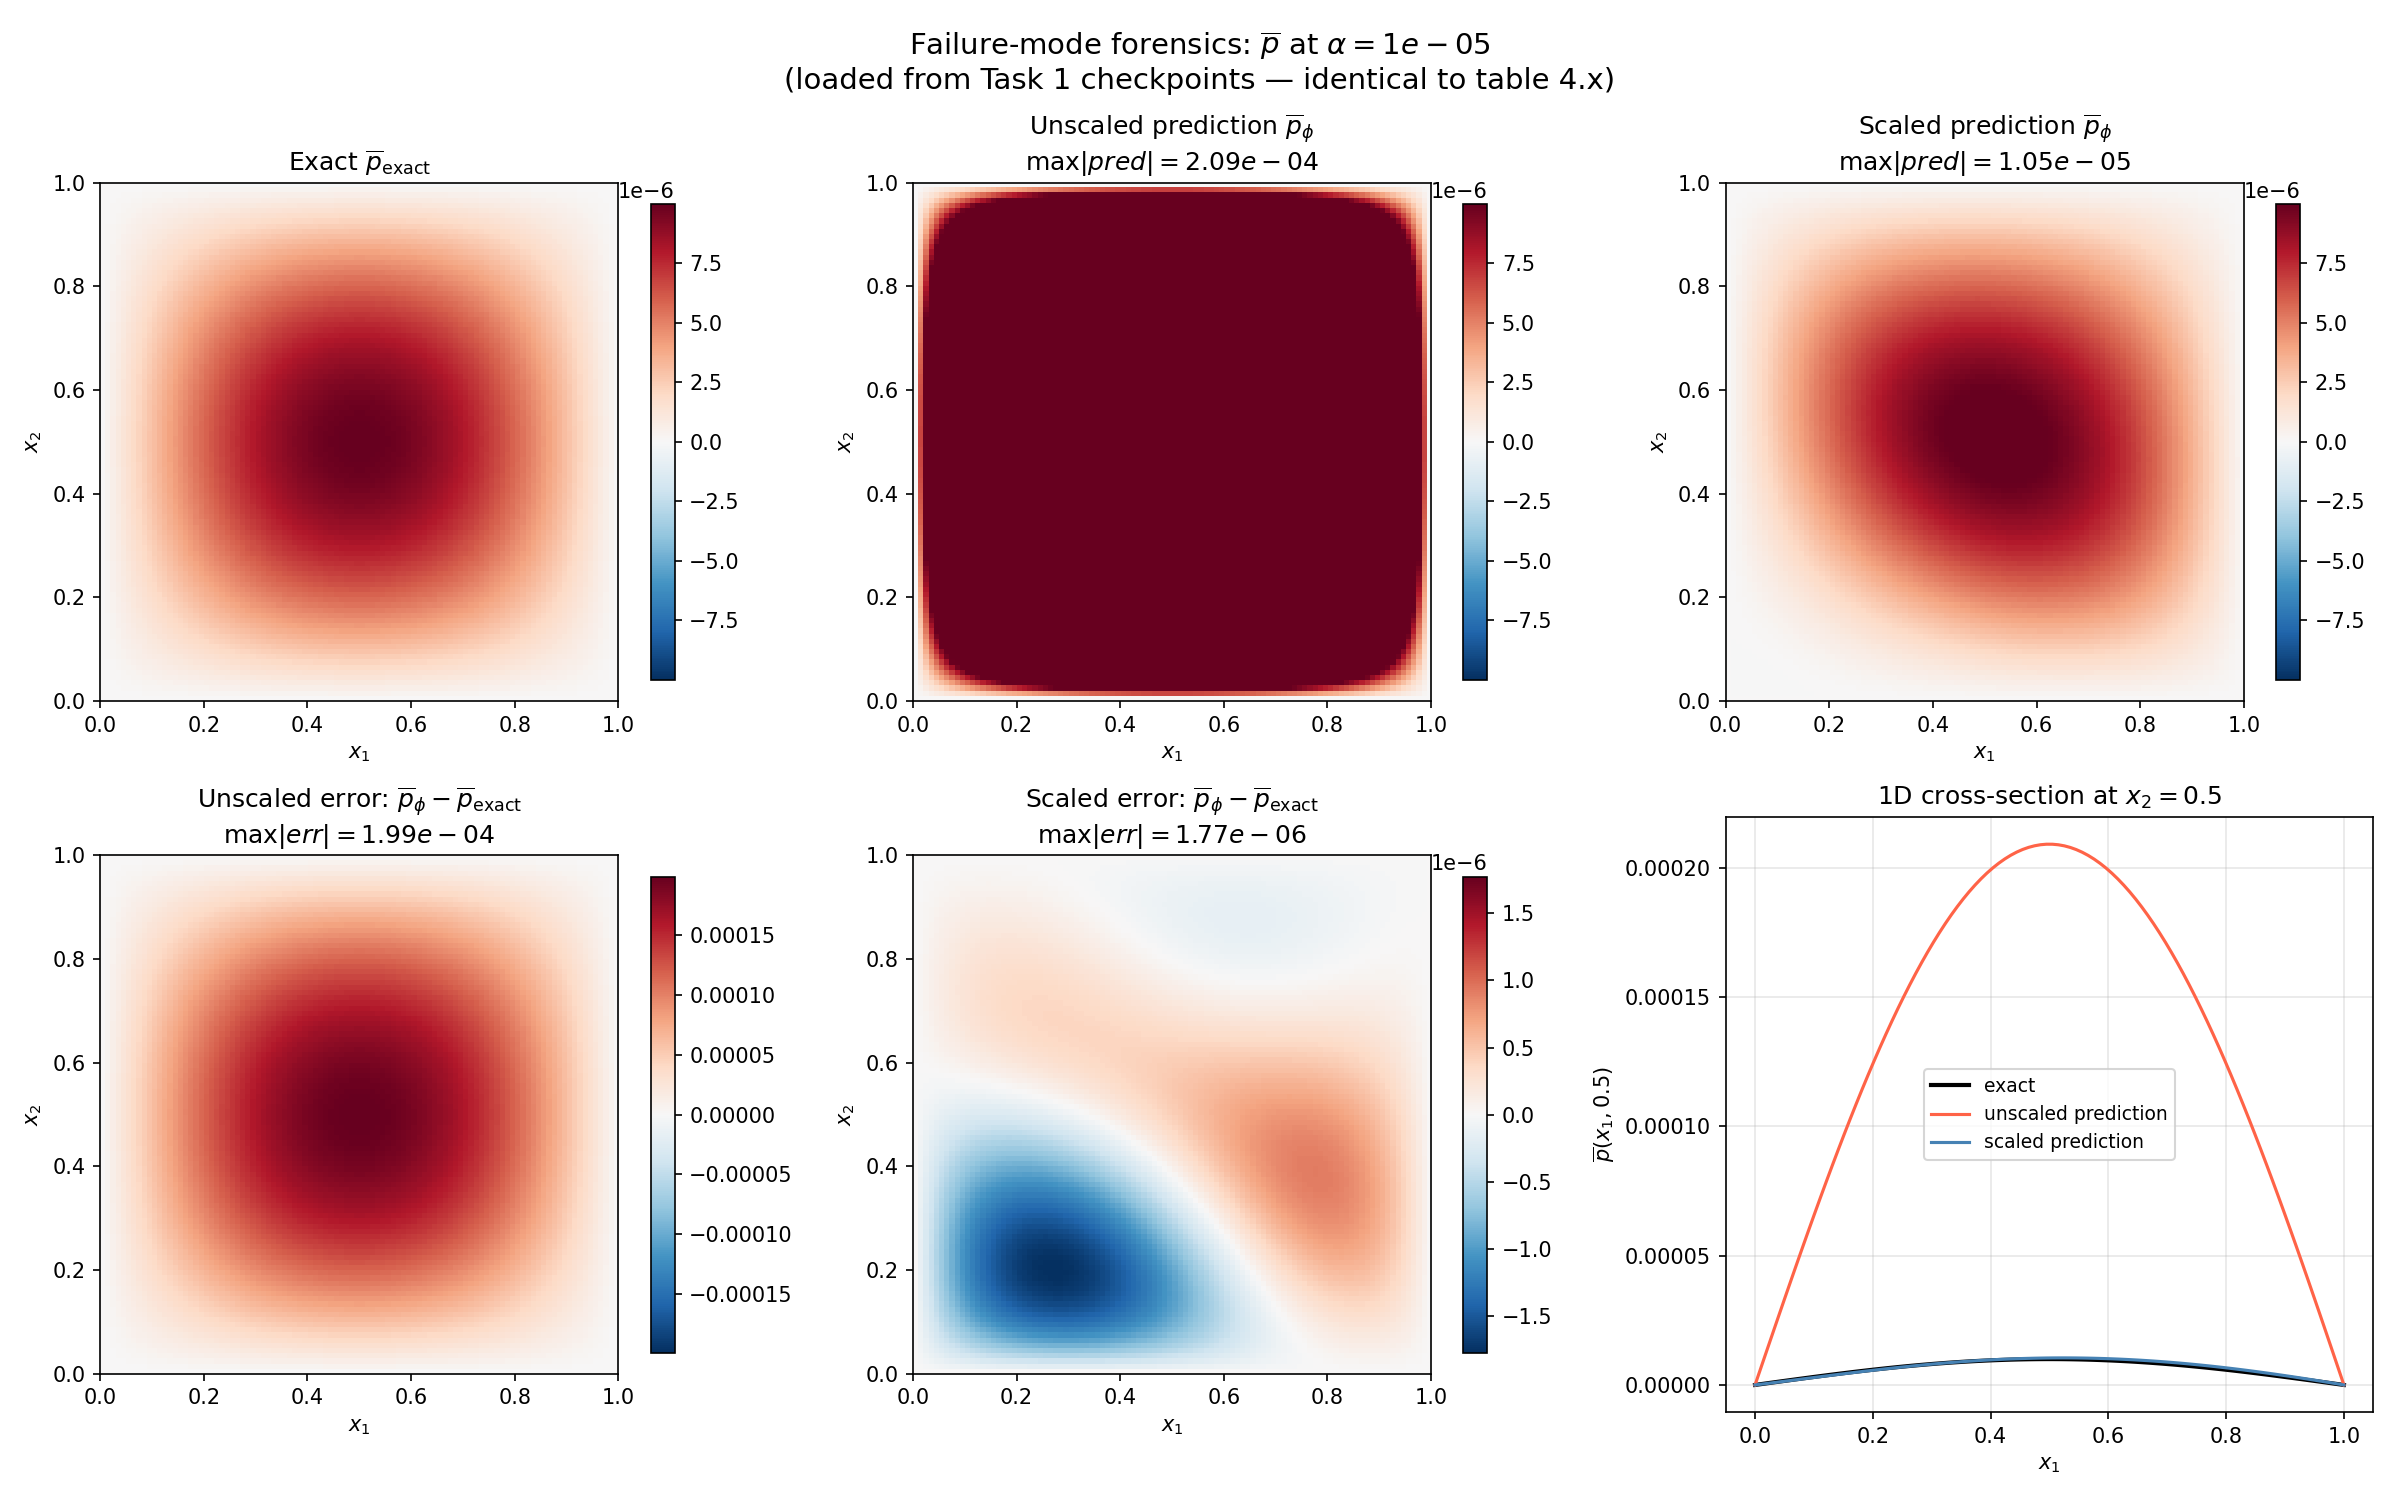
\includegraphics[width=\linewidth]{failure_mode_p.png}
  \caption{同一单元格下伴随变量 $\bar p$ 预测场的对比。
  Unscaled 预测 $\max|\bar p_\phi| = 2.09\times 10^{-4}$，
  是精确解 $\max|\bar p_{\rm exact}|\approx 10^{-5}$ 的 $\sim 20$ 倍，
  幅度错误；Scaled 预测 $\max|\bar p_\phi| = 1.05\times 10^{-5}$，
  最大逐点误差 $1.77\times 10^{-6}$，与精确解一致。}
  \label{fig:forensic-p}
\end{figure}

\paragraph{失效机理。}
Unscaled 系统的失效不是收敛缓慢，而是陷入了损失面的一个
\emph{平凡核局部极小}。状态残差含耦合项 $\alpha^{-1}\bar p$：
任何非零 $\bar p_\phi$ 都会带来 $O(\alpha^{-1})$ 量级的惩罚，
优化器因此将 $\bar p_\phi$ 压向零；代入伴随残差
$-\Delta\bar p_\phi - \bar y_\phi + y_d = 0$，得
$-\bar y_\phi + y_d\approx 0$。训练同时要求状态残差
$-\Delta\bar y_\phi - f + u_d + \alpha^{-1}\bar p_\phi\approx 0$，
在 $\bar p_\phi\to 0$ 下退化为 $-\Delta\bar y_\phi\approx f - u_d$；
两条路径联合极小化的唯一可行平衡是\emph{同时}将 $\bar y_\phi$ 与
$\bar p_\phi$ 压向零——即图~\ref{fig:forensic-y} 所示的平凡核。
该失效直接对应 §\ref{subsubsec:jacobian} 中 $J_{12}$ 的 $\alpha^{-1}$
爆炸：当一个残差对一个子网络的灵敏度远超另一残差时，
优化器的唯一可行联合极小化方向就是平凡核。

\paragraph{关于表~\ref{tab:alpha-hard-dual} 中 Scaled 的 $L^2_p\sim 0.1$。}
图~\ref{fig:forensic-p} 同时解释了该数字的性质：
$\|\bar p_{\rm exact}\|\propto\alpha$ 使相对 $L^2_p$ 被小分母放大；
绝对误差仅 $O(10^{-6})$，一维切片显示 Scaled 预测与精确解逐点重合。
这是度量本身的尺度伪影，而非学习质量的下降。

% ==================================================================

\xmusection{与自适应加权方法的对比}{Comparison with Adaptive Weighting}
\label{subsec:ntk}

PINN 文献中一种经典的替代路径是 Wang-Teng-Perdikaris~\cite{27} 的
NTK 自适应加权：不改造方程，而在训练中根据 NTK 迹动态调整损失权重，
更新规则为
\[
  \lambda_k^{\rm new} = \frac{\sum_i \mathrm{Tr}(K_i)}
                              {N_{\rm eq}\,\mathrm{Tr}(K_k)},
\]
其中 $K_k$ 为第 $k$ 个残差的 NTK。为考察 Scaling 与该类方法的关系，
在\emph{未缩放}系统 (1.17) 上实施 NTK 自适应加权（Hutchinson 迹估计，
EMA 系数 $0.9$，每 $100$ 步更新），扫描相同的
$\alpha\in\{10^{-2},\ldots,10^{-5}\}$（图~\ref{fig:ntk}）。

\begin{figure}[H]
  \centering
  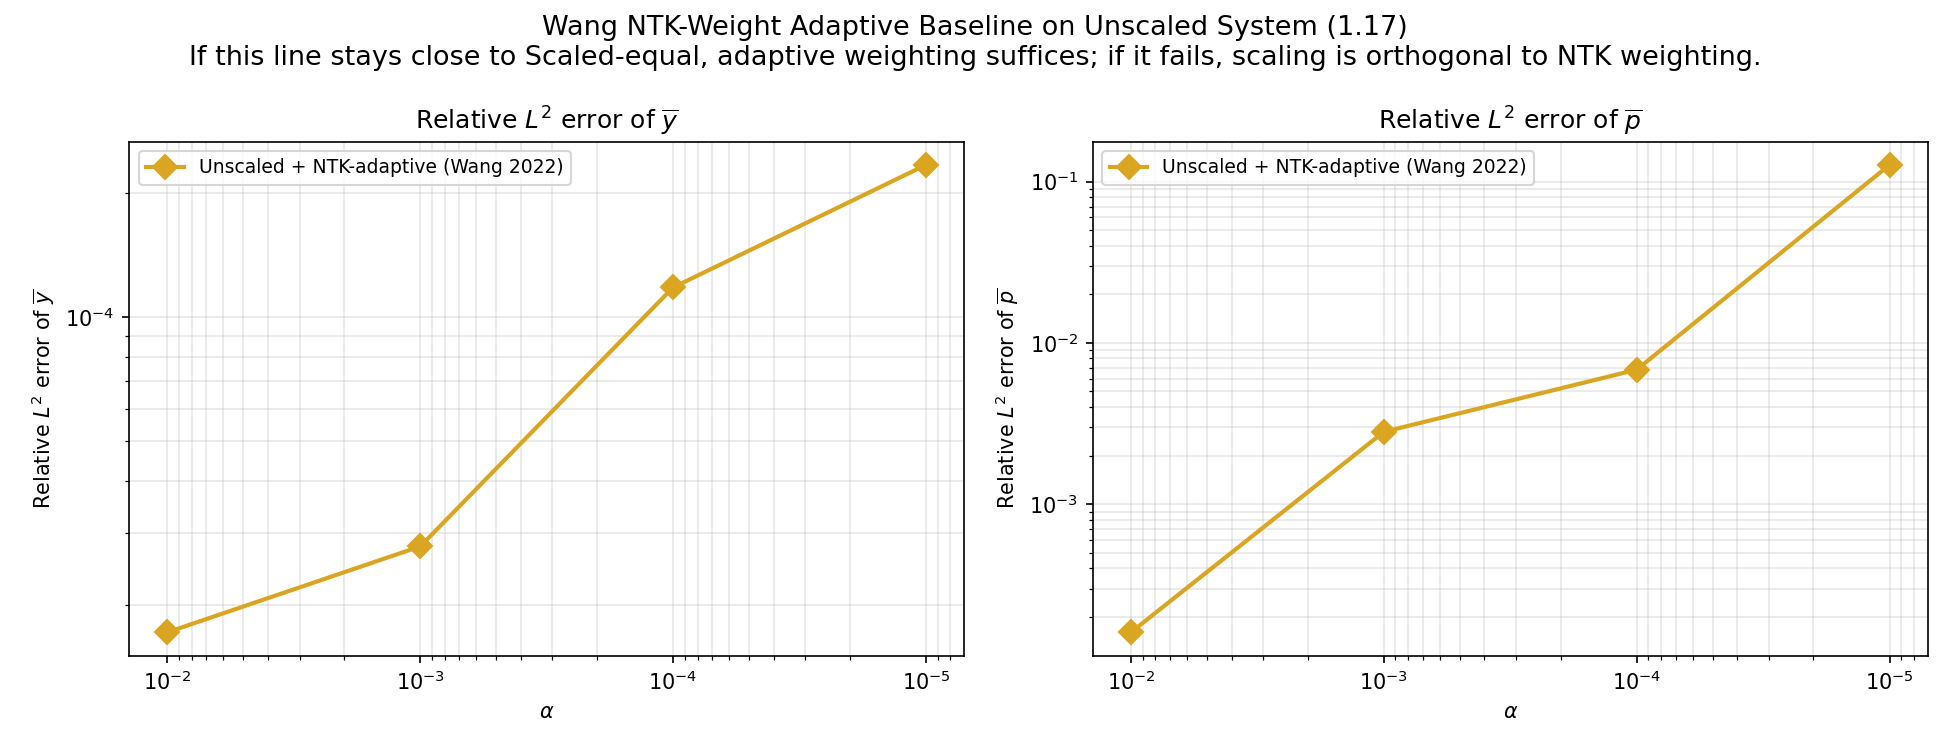
\includegraphics[width=\linewidth]{wang_ntk_baseline_result.png}
  \caption{未缩放系统 (1.17) + Wang NTK 自适应加权~\cite{27}
  的相对 $L^2$ 误差（Hard BC + Dual Network）。$\alpha\ge 10^{-3}$ 时
  与 Scaled + 等权精度相当；$\alpha\to 10^{-5}$ 时显著退化至
  $L^2_y\sim 10^{-3}$、$L^2_p\sim 10^{-1}$。}
  \label{fig:ntk}
\end{figure}

三种方法在 $\alpha = 10^{-5}$ 下的定量对比见表~\ref{tab:method-compare}。

\begin{table}[H]
  \centering
  \caption{三种方法在 $\alpha = 10^{-5}$、Hard BC + Dual Network 下的对比}
  \label{tab:method-compare}
  \small
  \begin{tabular}{l rr l c}
  \toprule
  方法 & $L^2_y$ & $L^2_p$ & 调参项 & 单步开销 \\
  \midrule
  Unscaled + 等权                         & $1.00\times 10^{+0}$ & $1.22\times 10^{+1}$ & 无 & -- \\
  Unscaled + NTK 自适应~\cite{27}         & $\sim\!10^{-3}$       & $\sim\!10^{-1}$       & EMA、更新周期、探针数 & $\sim +25\%$ \\
  Scaled + 等权（本文）                    & $1.92\times 10^{-3}$  & $1.24\times 10^{-1}$  & 无 & -- \\
  \bottomrule
  \end{tabular}
\end{table}

\paragraph{定位。}
三条路径处理同一病态的不同机制：
\begin{itemize}
  \item \textbf{Unscaled + 等权}：不作任何处理，$\alpha\le 10^{-4}$
        完全失效（平凡核塌缩）。
  \item \textbf{Unscaled + NTK 自适应}：在\emph{训练中}动态校正权重，
        等价于沿梯度流动态注入 Scaling 的效果；代价为三个超参数
        （EMA 系数、更新周期、Hutchinson 探针数）与每步
        $\sim 25\%$ 的 NTK 迹估计开销。
  \item \textbf{Scaled + 等权}（本文）：在\emph{连续层面}通过代数变换
        一次性消除病态；零超参数、零运行时开销，并有连续层面的
        inf-sup 稳定性定理保障（见第三章）。
\end{itemize}
两条路径并不冲突：NTK 自适应在不改方程的前提下工作，
Scaling 从源头消除病态。本文方法定位为后者。

% ==================================================================

\xmusection{综合讨论}{Synthesis}
\label{subsec:synthesis}

\paragraph{原理层与现象层的一一对应。}
§\ref{subsec:principle} 的诊断与 §\ref{subsec:phenomenon} 的误差表
之间存在一一对应：
\begin{itemize}
  \item $\|J_{12}\|_F\sim\alpha^{-1}$
        （图~\ref{fig:block-norms}）$\Rightarrow$ $\alpha\to 0$ 时
        未缩放 $L^2$ 误差发散（图~\ref{fig:alpha-hard-dual}）；
  \item 未缩放 $\rho_\omega$ 远离平衡
        （图~\ref{fig:rho-omega}）$\Rightarrow$ $\omega$-扫描失败
        （图~\ref{fig:omega-hard-dual}）；
        
\end{itemize}

\paragraph{Hard BC 与 Soft BC}
Hard BC 下距离函数 Ansatz 精确满足边界条件，是 Scaling 效果的上限
（$L^2\sim 10^{-4}$）；Soft BC 下绝对精度降低约 $1$--$2$ 个数量级
（$L^2\sim 10^{-2}$），但在 $w_{bc}\ge 10$ 下 Scaling 的相对优势
依然显著。在实际应用中，复杂几何使 Hard BC 不可用时，
Soft BC + Scaling + 边界归一化的组合仍能保证数量级的改进。

\paragraph{双网络与单一网络}
全部主体实验使用 Dual Network 以排除参数共享对 $\alpha$-病态的混杂。
我们在 Hard BC 下额外检验了 Unified Network（单一网络输出
$(\bar y_\phi, \bar p_\phi)$），定性结论完全一致：Unscaled 在
$\alpha\le 10^{-4}$ 彻底失效，Scaled 在全 $\alpha$ 范围稳定于
$L^2\sim 10^{-3}$；Unified 下 Scaled 的 $L^2_p$ 因参数共享带来的隐式
耦合而略优于 Dual 约一个数量级。这说明 Scaling 的结构性修复
与网络架构选择无关。在此仅使用 Dual 作为主体以使 $\alpha$-病态的影响
干净可见。

\paragraph{$L^2$ 与 $H^1$ 误差数值相近的原因\cite{32}}
在 PINN 训练良好的场景中，网络能准确学到解的形状，往往仅在\emph{幅度}
上差一个极小比例 $\epsilon$：
\[
  u_\phi(x) \approx (1 - \epsilon)\,u_{\rm exact}(x),
\]
此时误差函数 $e(x) = u_\phi(x) - u_{\rm exact}(x) = -\epsilon\,u_{\rm exact}(x)$，
误差梯度亦正比于精确解梯度 $\nabla e(x) = -\epsilon\,\nabla u_{\rm exact}(x)$。
代入相对 $L^2$ 与 $H^1$ 误差：
\begin{align*}
  e_{L^2}
   &= \sqrt{\frac{\|e\|_{L^2}^2}{\|u_{\rm exact}\|_{L^2}^2}}
    = \sqrt{\frac{\epsilon^2\|u_{\rm exact}\|_{L^2}^2}{\|u_{\rm exact}\|_{L^2}^2}}
    = \epsilon,\\
  e_{H^1}
   &= \sqrt{\frac{\|e\|_{L^2}^2 + \|\nabla e\|_{L^2}^2}
                 {\|u_{\rm exact}\|_{L^2}^2 + \|\nabla u_{\rm exact}\|_{L^2}^2}}
    = \sqrt{\frac{\epsilon^2\bigl(\|u_{\rm exact}\|_{L^2}^2 + \|\nabla u_{\rm exact}\|_{L^2}^2\bigr)}
                 {\|u_{\rm exact}\|_{L^2}^2 + \|\nabla u_{\rm exact}\|_{L^2}^2}}
    = \epsilon.
\end{align*}
故 $L^2$ 与 $H^1$ 数值几乎相同。更深层地，由 Sobolev 空间的椭圆正则性
定理，对泊松方程 $-\Delta e = r$（$r$ 为残差）存在常数 $C_1$ 满足
$\|e\|_{H^2}\le C_1\|r\|_{L^2}$——这意味着只要 PINN 将 PDE 残差
压低，误差的二阶导数即被自动界定，$L^2$ 与 $H^1$ 误差自然随之同步
下降了。

\paragraph{$L^\infty$ 范数的差异化表现}
$L^\infty$ 作为由局部极值决定的最大值范数，不同于 $L^2$、$H^1$ 这类
全局相对范数。在失效边界单元格（$\alpha = 10^{-5}$ 下的 Unscaled）中，
$L^\infty$ 对平凡核塌缩最为敏感——网络预测整体接近零时，
$L^\infty$ 误差精确等于 $\max|u_{\rm exact}|$，直接暴露失效严重程度；
这也是 §\ref{subsec:forensics} 使用 $\max|\mathrm{pred}|$
与 $\max|\mathrm{err}|$ 的图示，而非相对 $L^2$ 的原因。

\begin{remark}[关于 $L^\infty_p$ 的非单调表现]
图~\ref{fig:alpha-hard-dual} 中段 $L^\infty_p$ 的缩放曲线在
$\alpha = 10^{-3}$ 出现小凸起后急剧下降——这并非异常：
$\bar p_{\rm exact} = \alpha \bar y$ 幅度正比于 $\alpha$，绝对误差随之
衰减，故 $L^\infty_p$（绝对误差）作为 $\alpha$ 的函数呈单调下降趋势，
与相对 $L^2$、$H^1$ 指标形成对照。
\end{remark}


% 参考文献

\begin{reference}
    % 已自动按照 GB/T 7714-2005 设置参考文献的引用格式
    \begin{thebibliography}{99}
    \bibitem[1]{1}
    F.~Tröltzsch,
    \textit{Optimal Control of Partial Differential Equations: Theory, Methods, and Applications},
    Graduate Studies in Mathematics, vol. 112, American Mathematical Society, 2010.

    \bibitem[2]{3}
    W.~Gong, Z.~Tan, and Z.~Zhou,
    Optimal convergence of finite element approximation to an optimization problem with PDE constraint,
    \textit{Inverse Problems}, vol.~38, no.~4, 045004, 2022.

    \bibitem[3]{4}
    S.~C.~Brenner, S.~Liu, and L.-y.~Sung,
    Multigrid methods for saddle point problems: Karush--Kuhn--Tucker systems,
    arXiv preprint arXiv:1811.12434, 2018.

    \bibitem[4]{5}
    M.~Weng, Z.~Mao, and J.~Shen,
    Deep collocation method: A framework for solving PDEs using neural networks with error control,
    \textit{SIAM J. Sci. Comput.}, vol.~48, no.~1, C77--C102, 2026.

    \bibitem[5]{6}
    Michael Feischl.
    \textit{Inf-sup stability implies quasi-orthogonality}.
    arXiv:2008.12198 [math.NA], 2022.
    URL: \url{https://arxiv.org/abs/2008.12198}.

    \bibitem[6]{16}
    L.~Lu, R.~Pestourie, W.~Yao, Z.~Wang, F.~Verdugo, and S.~G.~Johnson,
    Physics-informed neural networks with hard constraints for inverse design,
    \textit{SIAM J. Sci. Comput.}, vol.~43, no.~6, B1105--B1132, 2021.

    \bibitem[7]{21}
    M.~Raissi, P.~Perdikaris, and G.~E.~Karniadakis,
    Physics-informed neural networks: A deep learning framework for solving forward and inverse problems involving nonlinear partial differential equations,
    \textit{J. Comput. Phys.}, vol.~378, 686--707, 2019.

    \bibitem[8]{22}
    A.~G.~Baydin, B.~A.~Pearlmutter, A.~A.~Radul, and J.~M.~Siskind,
    Automatic differentiation in machine learning: A survey,
    \textit{J. Mach. Learn. Res.}, vol.~18, no.~153, 1--43, 2018.

    \bibitem[9]{23}
    E.~Lagaris, A.~Likas, and D.~I.~Fotiadis,
    Artificial neural networks for solving ordinary and partial differential equations,
    \textit{IEEE Trans. Neural Netw.}, vol.~9, no.~5, 987--1000, 1998.

    \bibitem[10]{24}
    S.~Dong and N.~Ni,
    A method for representing a solution of elliptic boundary value problems with an approximate solution satisfying the boundary conditions exactly,
    \textit{J. Comput. Phys.}, vol.~444, 110545, 2021.

    \bibitem[11]{25}
    D.~P.~Kingma and J.~Ba,
    Adam: A method for stochastic optimization,
    in \textit{Proceedings of the 3rd International Conference on Learning Representations (ICLR)}, 2015.

    \bibitem[12]{26}
    D.~C.~Liu and J.~Nocedal,
    On the limited memory BFGS method for large scale optimization,
    \textit{Math. Program.}, vol.~45, no.~1, 503--528, 1989.

    \bibitem[13]{27}
    S.~Wang, Y.~Teng, and P.~Perdikaris,
    Understanding and mitigating gradient flow pathologies in physics-informed neural networks,
    \textit{SIAM J. Sci. Comput.}, vol.~43, no.~5, A3055--A3081, 2021.

    \bibitem[14]{28}
    K.~Hornik,
    Approximation capabilities of multilayer feedforward networks,
    \textit{Neural Netw.}, vol.~4, no.~2, 251--257, 1991.

    \bibitem[15]{29}
    S.~Wang, X.~Yu, and P.~Perdikaris,
    When and why PINNs fail to train: A neural tangent kernel perspective,
    \textit{J. Comput. Phys.}, vol.~449, 110768, 2022.

    \bibitem[16]{30}
    M.~F.~Hutchinson,
    A stochastic estimator of the trace of the influence matrix for Laplacian smoothing splines,
    \textit{Comm. Statist. Simulation Comput.}, vol.~19, no.~2, 433--450, 1990.

    \bibitem[17]{31}
    S.~Elfwing, E.~Uchibe, and K.~Doya,
    Sigmoid-weighted linear units for neural network function approximation in reinforcement learning,
    \textit{Neural Networks}, vol.~107, 3--11, 2018.

    \bibitem[18]{32}
    L.~C.~Evans,
    \textit{Partial Differential Equations},
    Graduate Studies in Mathematics, vol.~19, 2nd ed., American Mathematical Society, 2010.

    \bibitem[19]{33}
    E.~E.~Osborne,
    On pre-conditioning of matrices,
    \textit{J. ACM}, vol.~7, no.~4, 338--345, 1960.

    \end{thebibliography}{99}

    
\end{reference}

% 附录

\begin{appendix}
    附录内容。
\end{appendix}

% 如果想要将致谢放在最后，可将最前的致谢移动至此

\end{document}
